\documentclass[10pt]{beamer}

%STANDARD PREAMBLE
%https://tex.stackexchange.com/questions/68821/is-it-possible-to-create-a-latex-preamble-header
\usepackage{/Users/miw267/Repos/latex_preamble/beamer_preamble}
%\usepackage{/Users/miw267/Repos/csci246_spring2025/slides/preambles/beamer_preamble_for_CSCI246}


%%%
% SPECIFIC TO THIS DOCUMENT 
%%%
\usepackage{animate}

\renewcommand{\ELBO}{\texttt{ELBO}}
\renewcommand{\Q}{\mathcal{Q}}


%%%%
% DOCUMENT 
%%%
\title{04/14/2026: Transformers}
\author{Reference: Chris Bishop \textit{Deep Learning}, Chapter 12.}
\date{CSCI 546: Diffusion Models}

\begin{document}
\maketitle

%\begin{frame}{Table of contents}
%  \setbeamertemplate{section in toc}[sections numbered]
%  \tableofcontents[hideallsubsections]
%\end{frame}

\begin{frame}{Table of contents}
  \setbeamertemplate{section in toc}[sections numbered]
  \setbeamertemplate{subsection in toc}[subsections numbered]
  \tableofcontents
\end{frame}





\section{Course Logistics}



%\begin{frame}
%
%\red{TBD}
%
%	
%\end{frame}


\begin{frame}{Reading Survey \#8}

What is attention, and how does it work?

	
\end{frame}



%\section{Mini-Lecture: SDE's}
%
%\begin{frame}{Diffusion Process}
%\centering
%\only<1>{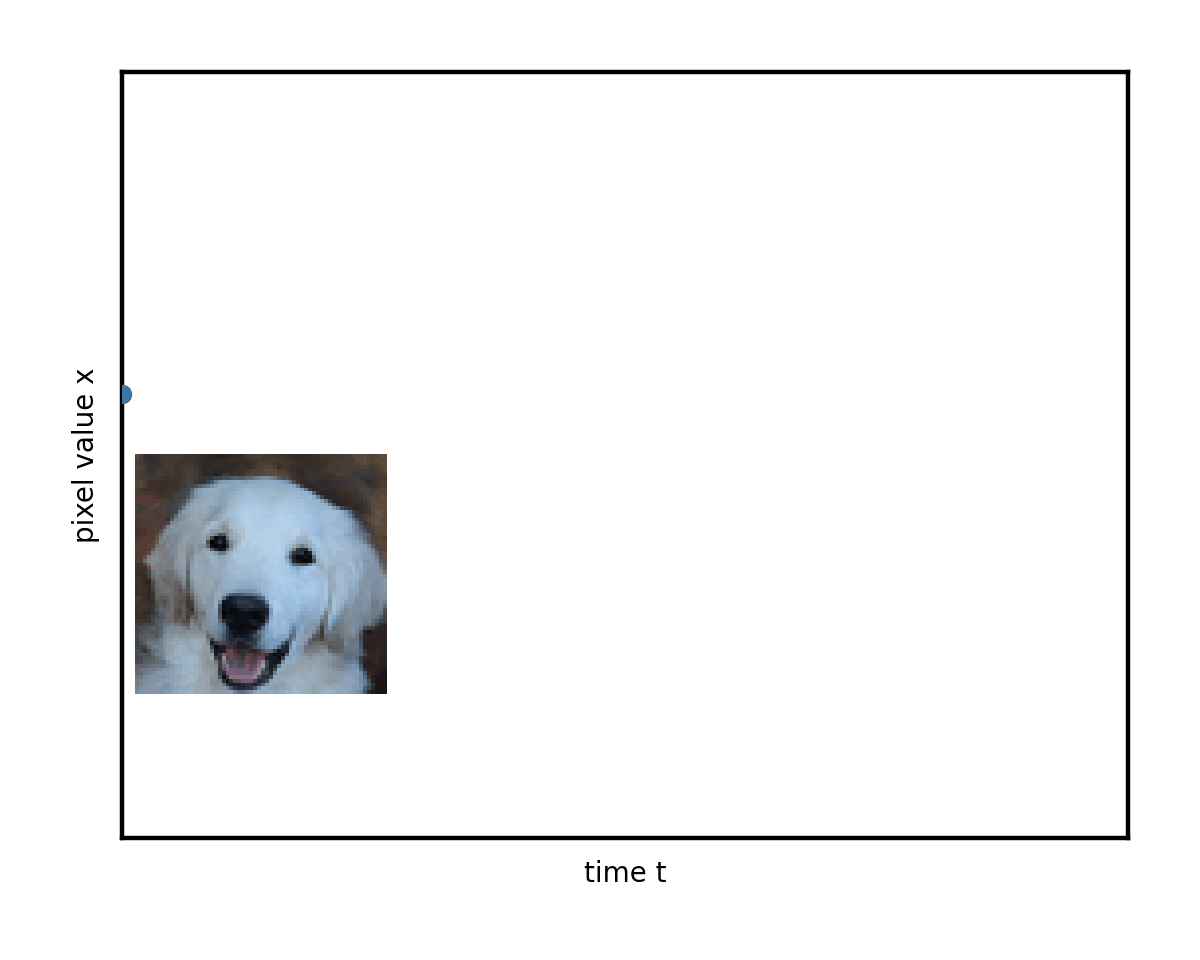
\includegraphics[width=0.85\textwidth]{frames/frame_000}}
%\only<2>{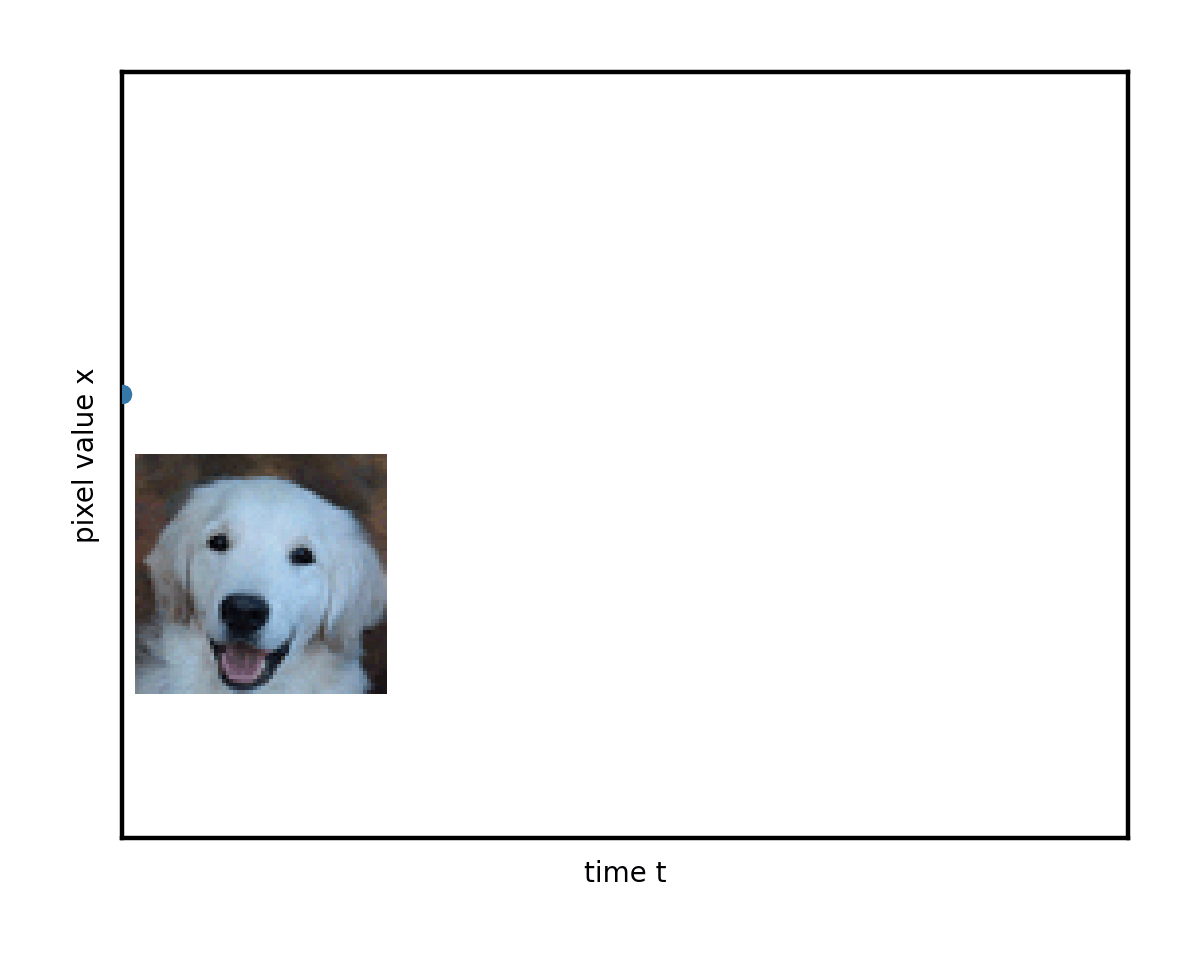
\includegraphics[width=0.85\textwidth]{frames/frame_001}}
%\only<3>{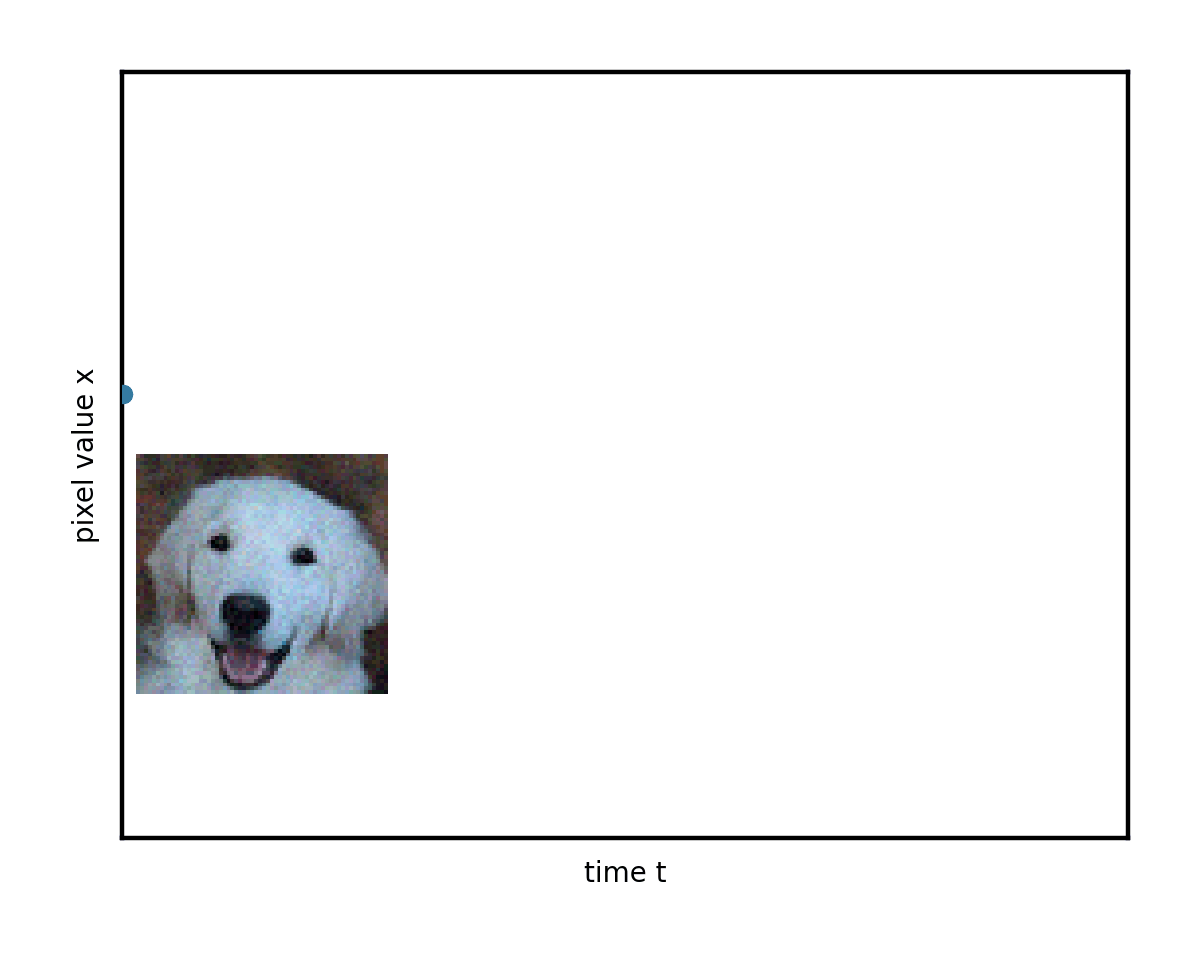
\includegraphics[width=0.85\textwidth]{frames/frame_002}}
%\only<4>{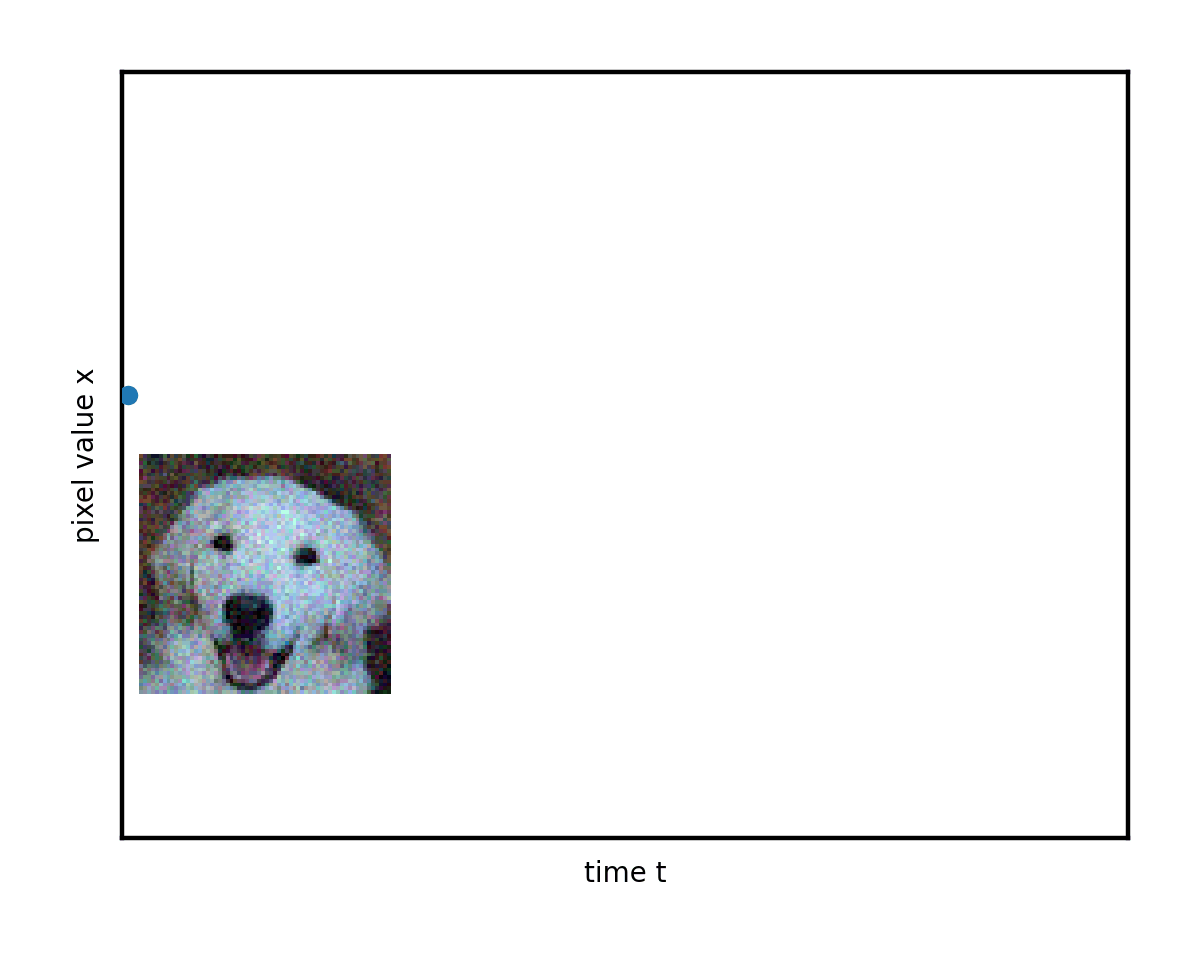
\includegraphics[width=0.85\textwidth]{frames/frame_003}}
%\only<5>{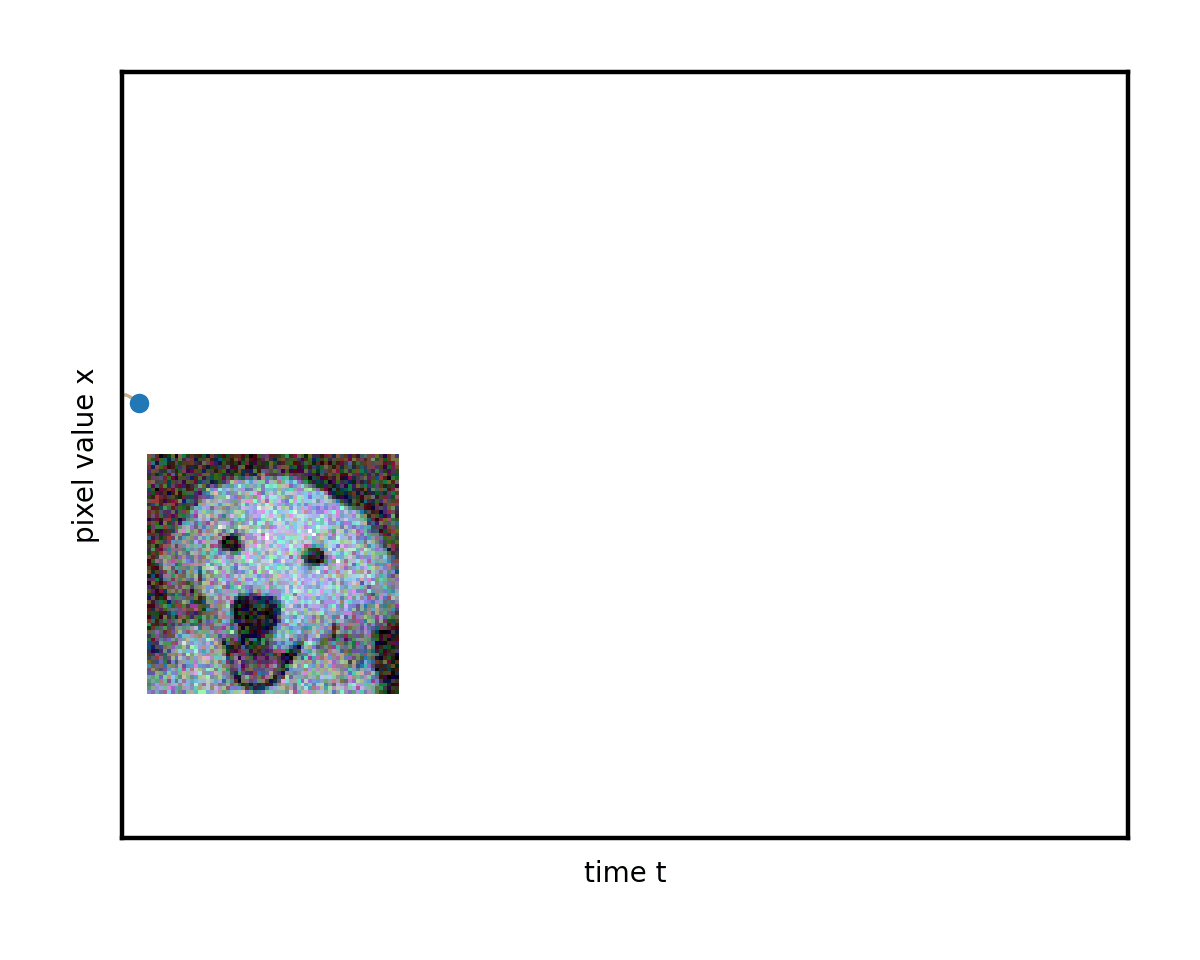
\includegraphics[width=0.85\textwidth]{frames/frame_004}}
%\only<6>{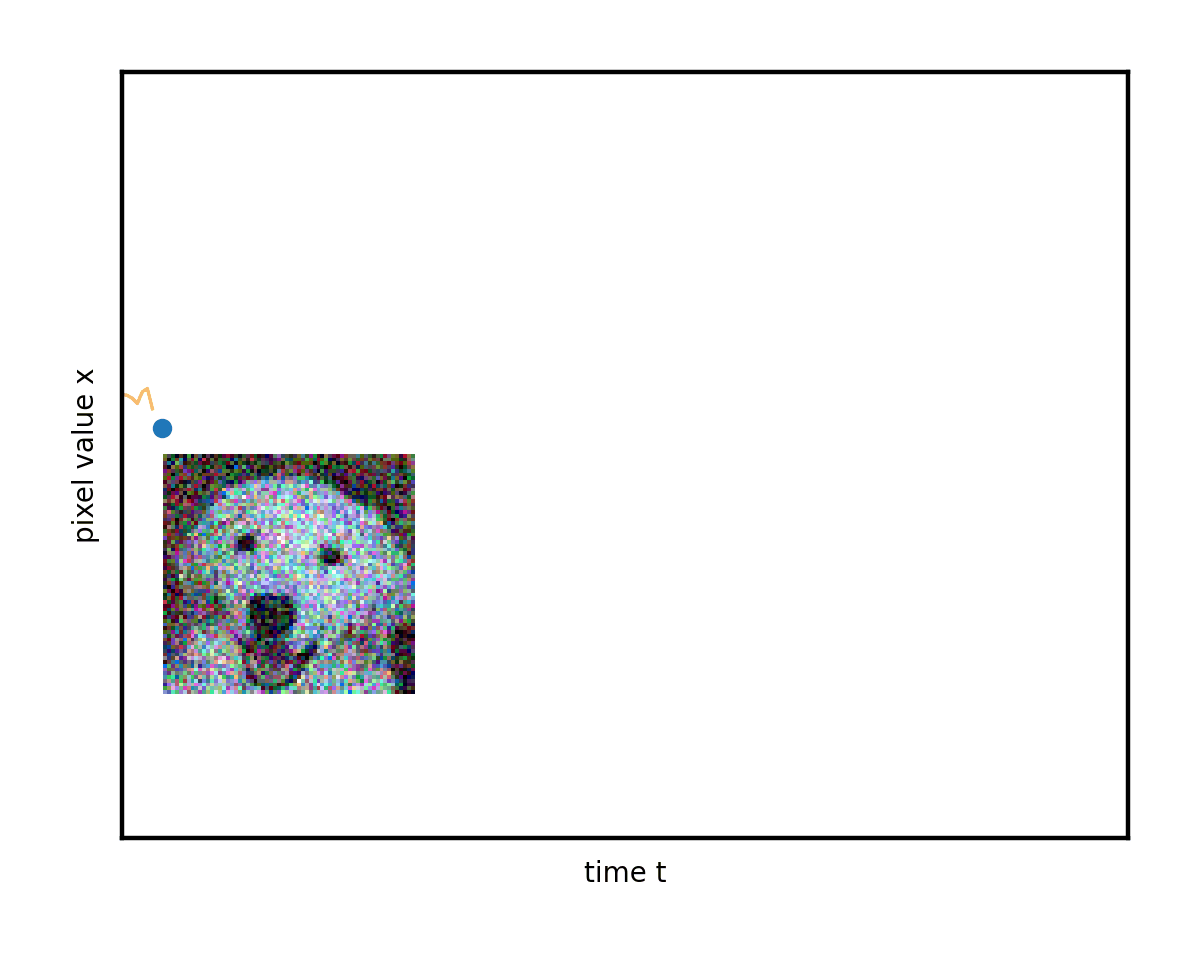
\includegraphics[width=0.85\textwidth]{frames/frame_005}}
%\only<7>{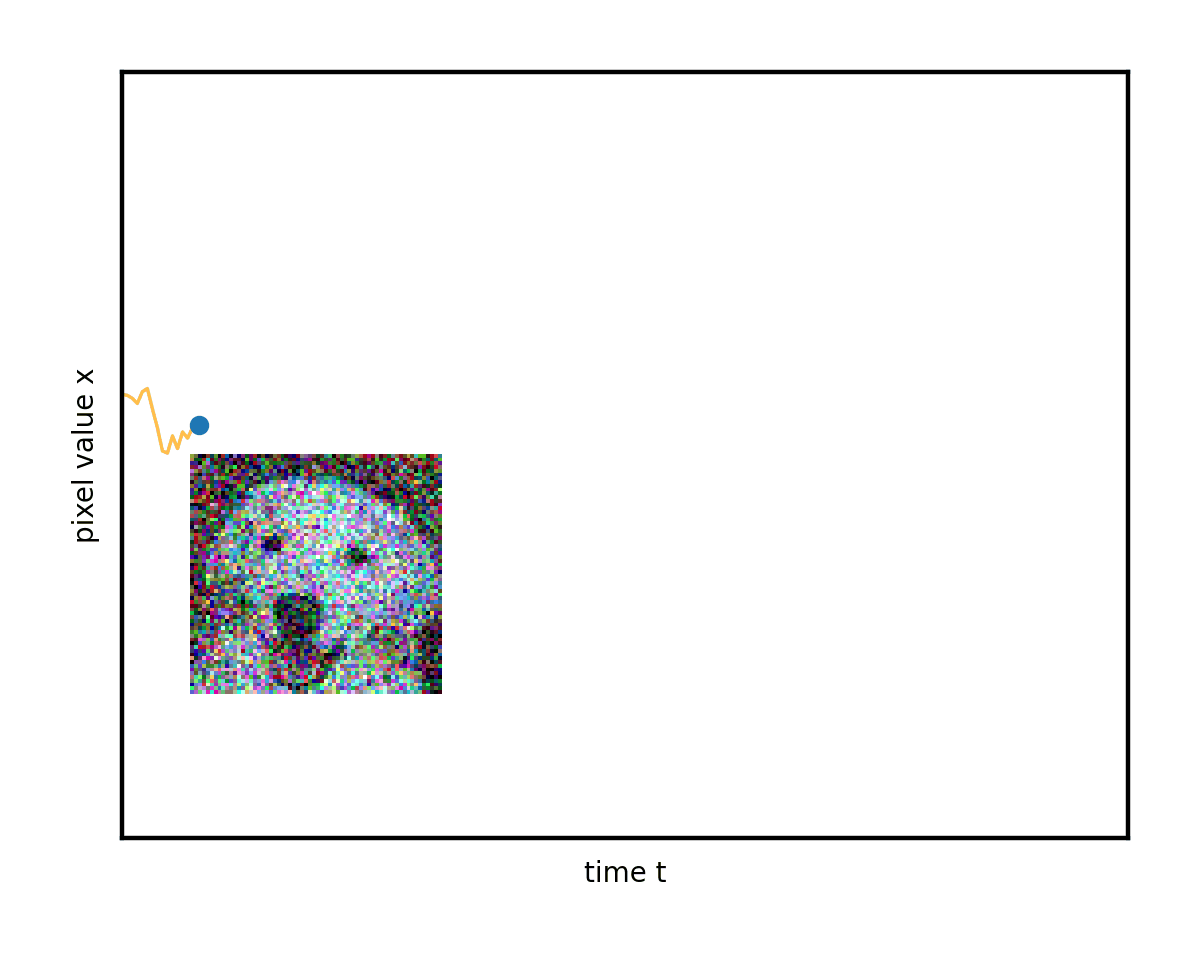
\includegraphics[width=0.85\textwidth]{frames/frame_006}}
%\only<8>{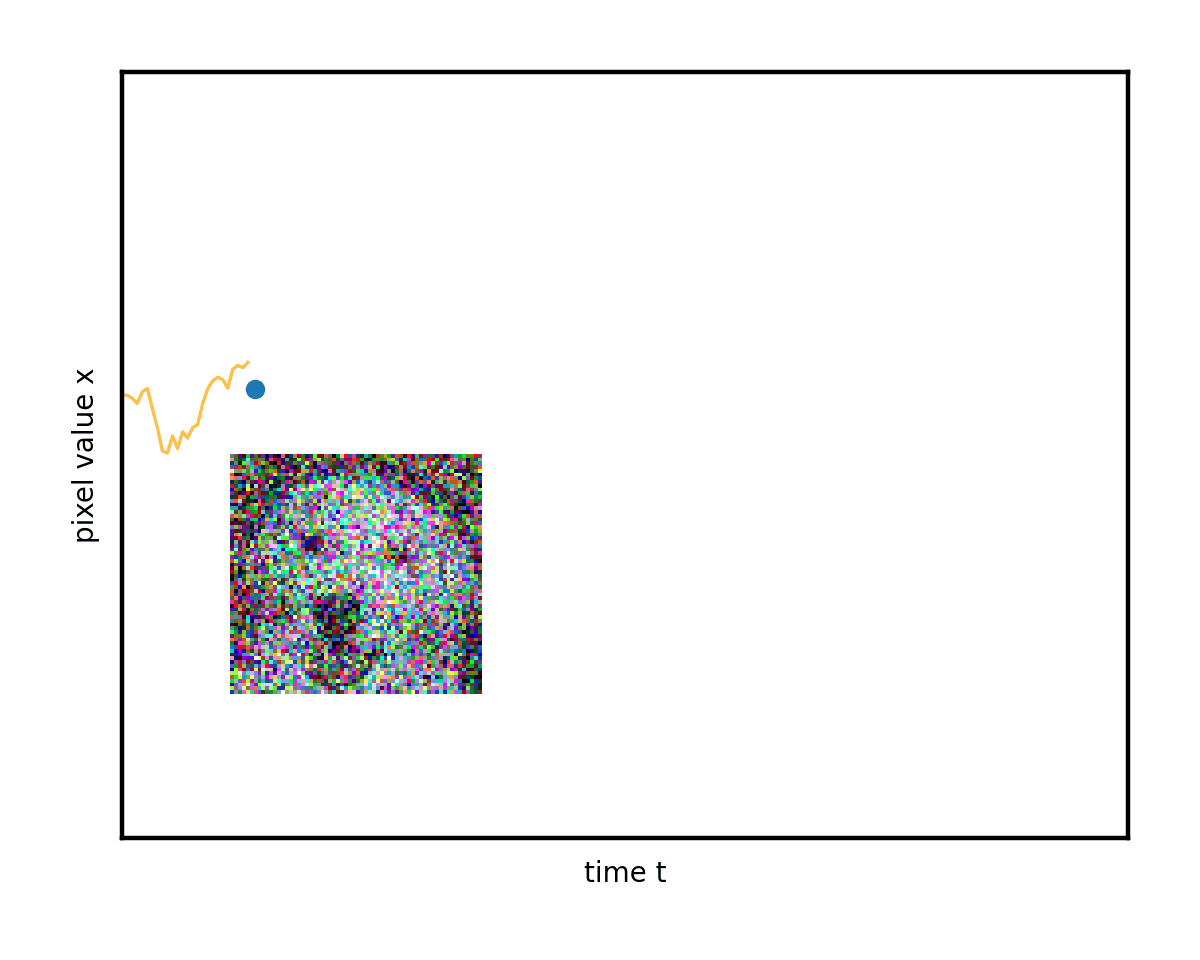
\includegraphics[width=0.85\textwidth]{frames/frame_007}}
%\only<9>{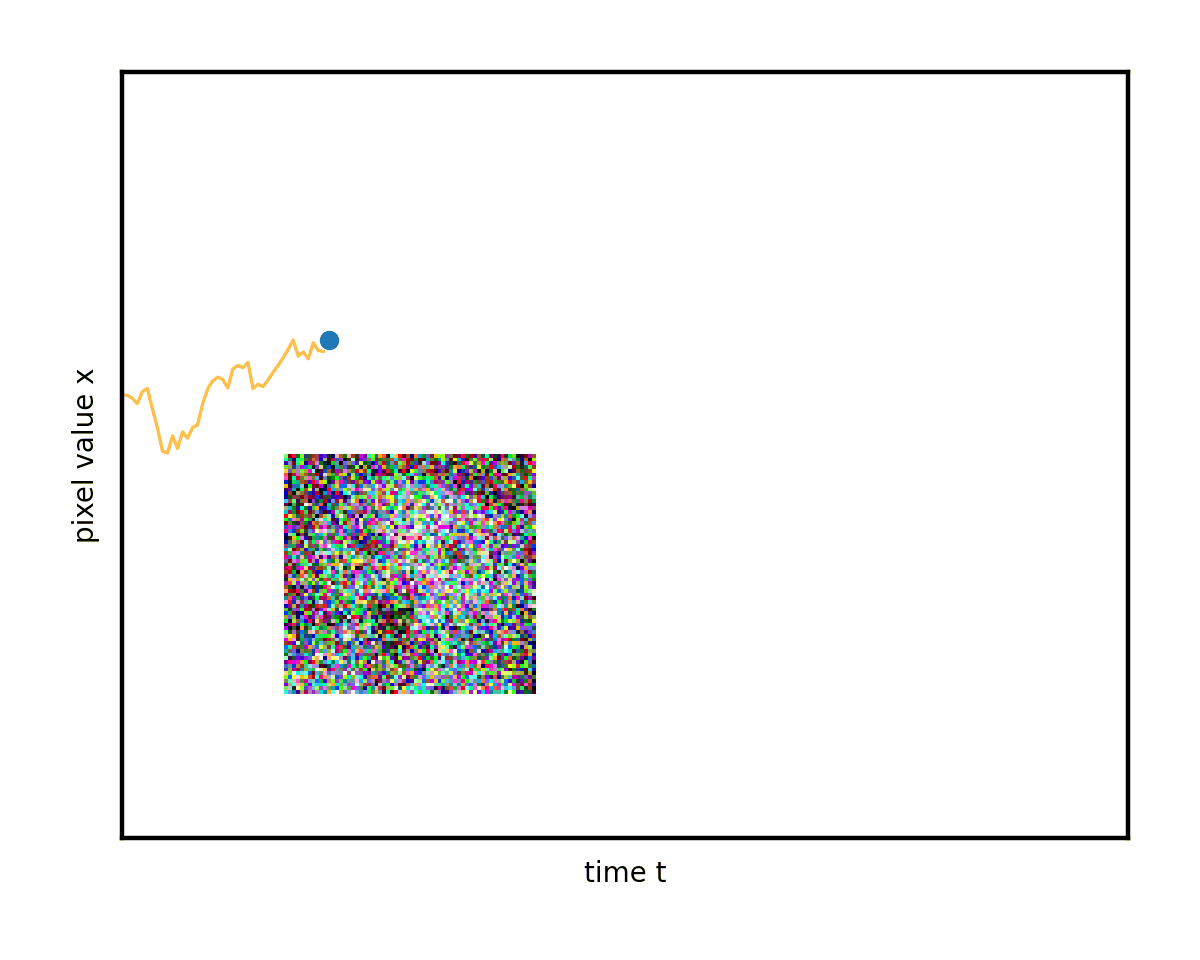
\includegraphics[width=0.85\textwidth]{frames/frame_008}}
%\only<10>{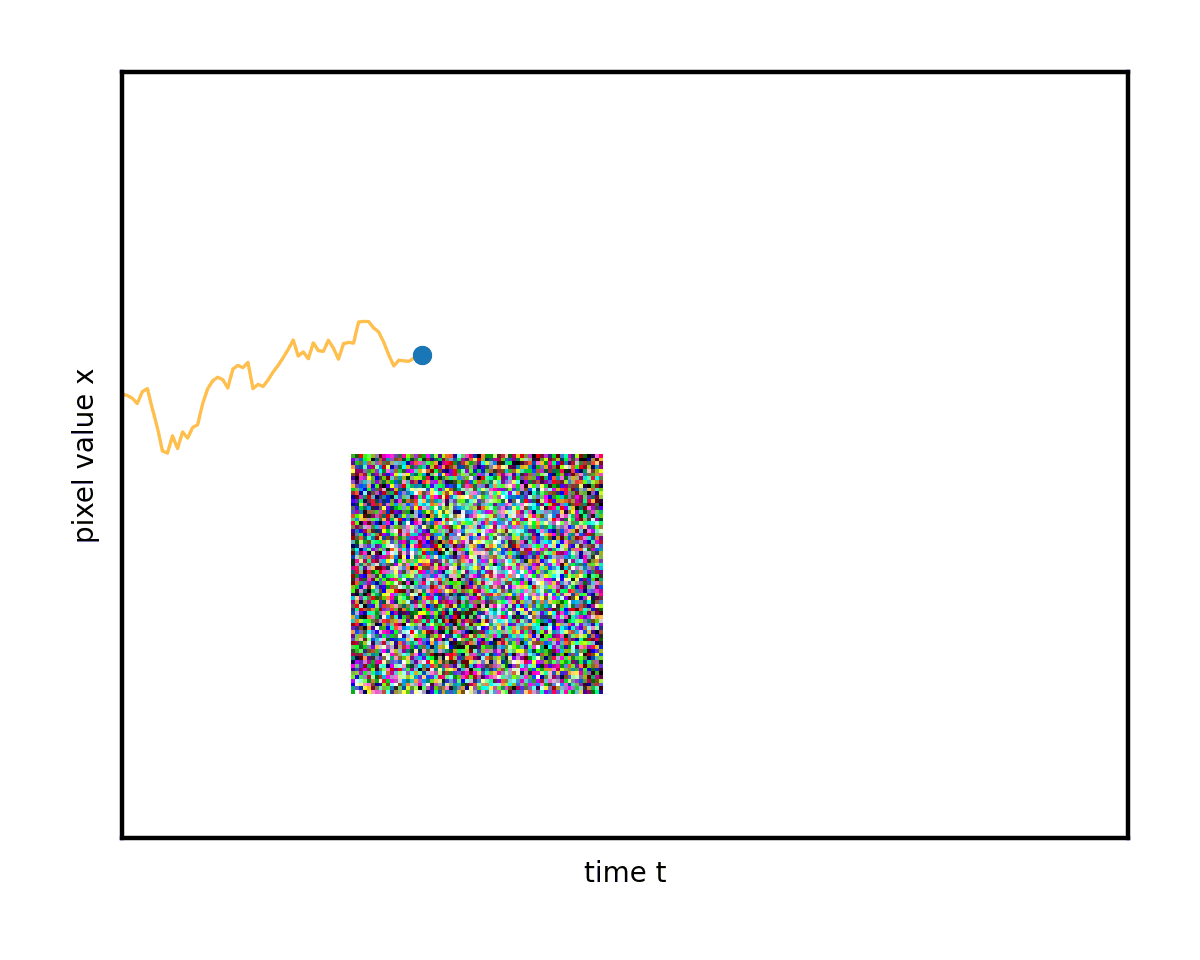
\includegraphics[width=0.85\textwidth]{frames/frame_009}}
%\only<11>{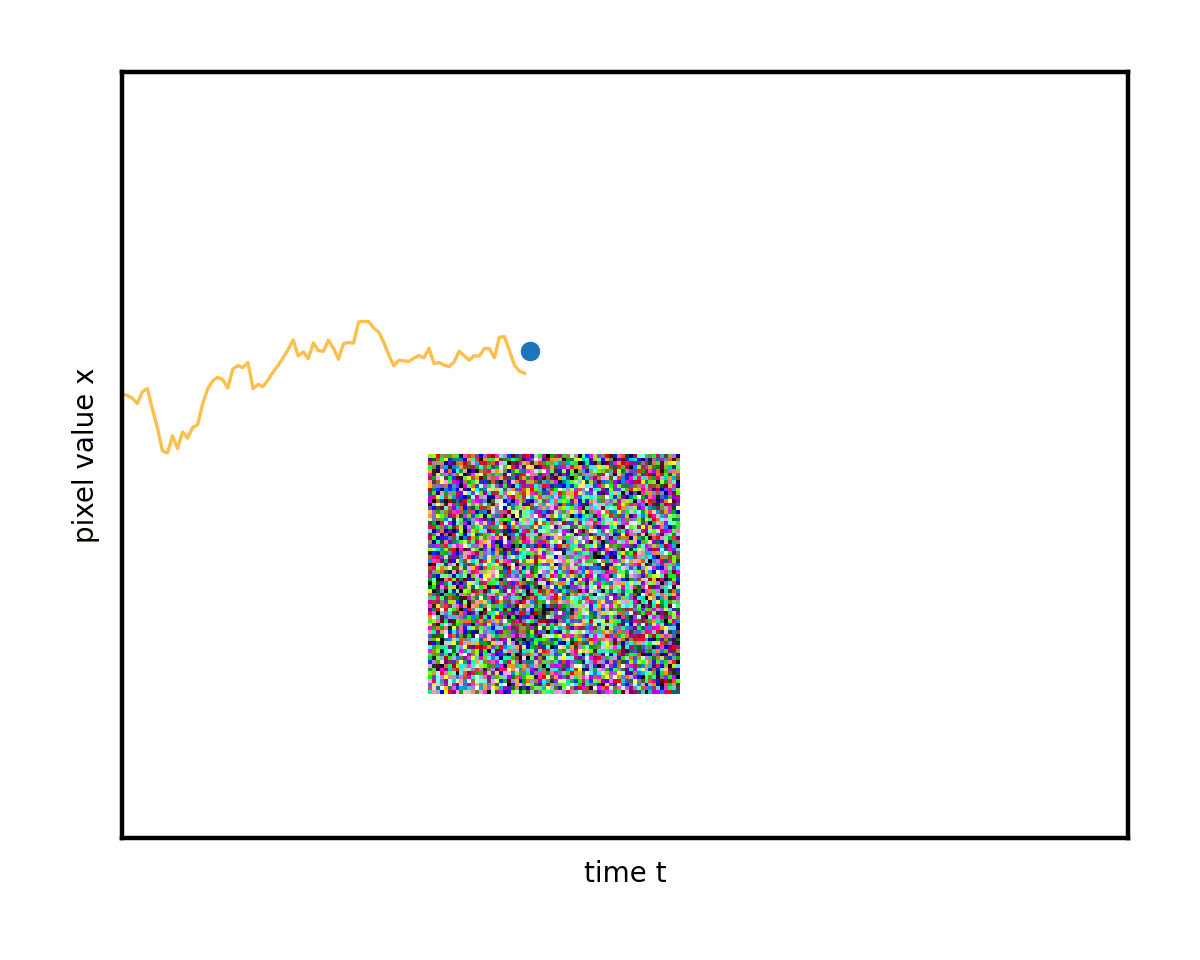
\includegraphics[width=0.85\textwidth]{frames/frame_010}}
%\only<12>{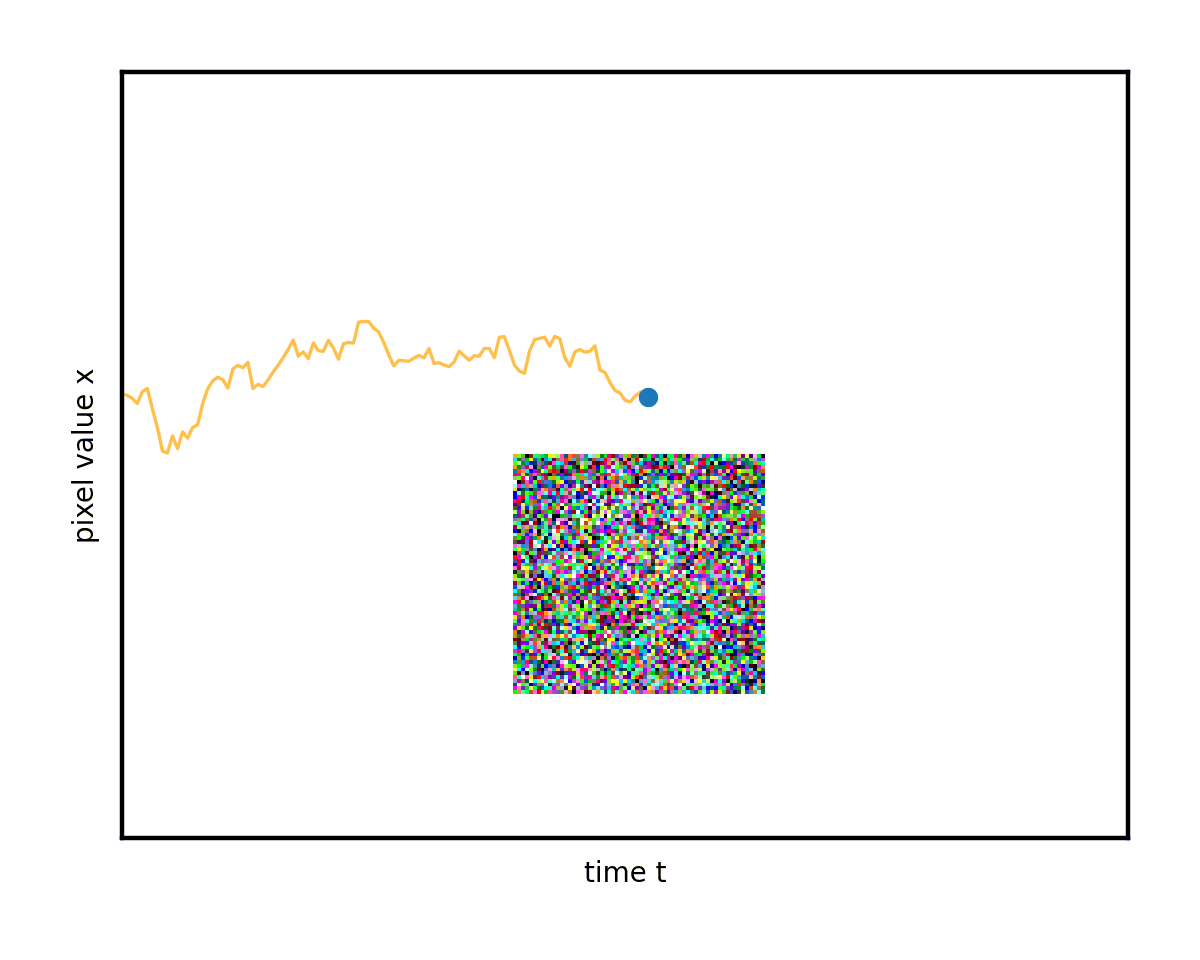
\includegraphics[width=0.85\textwidth]{frames/frame_011}}
%\only<13>{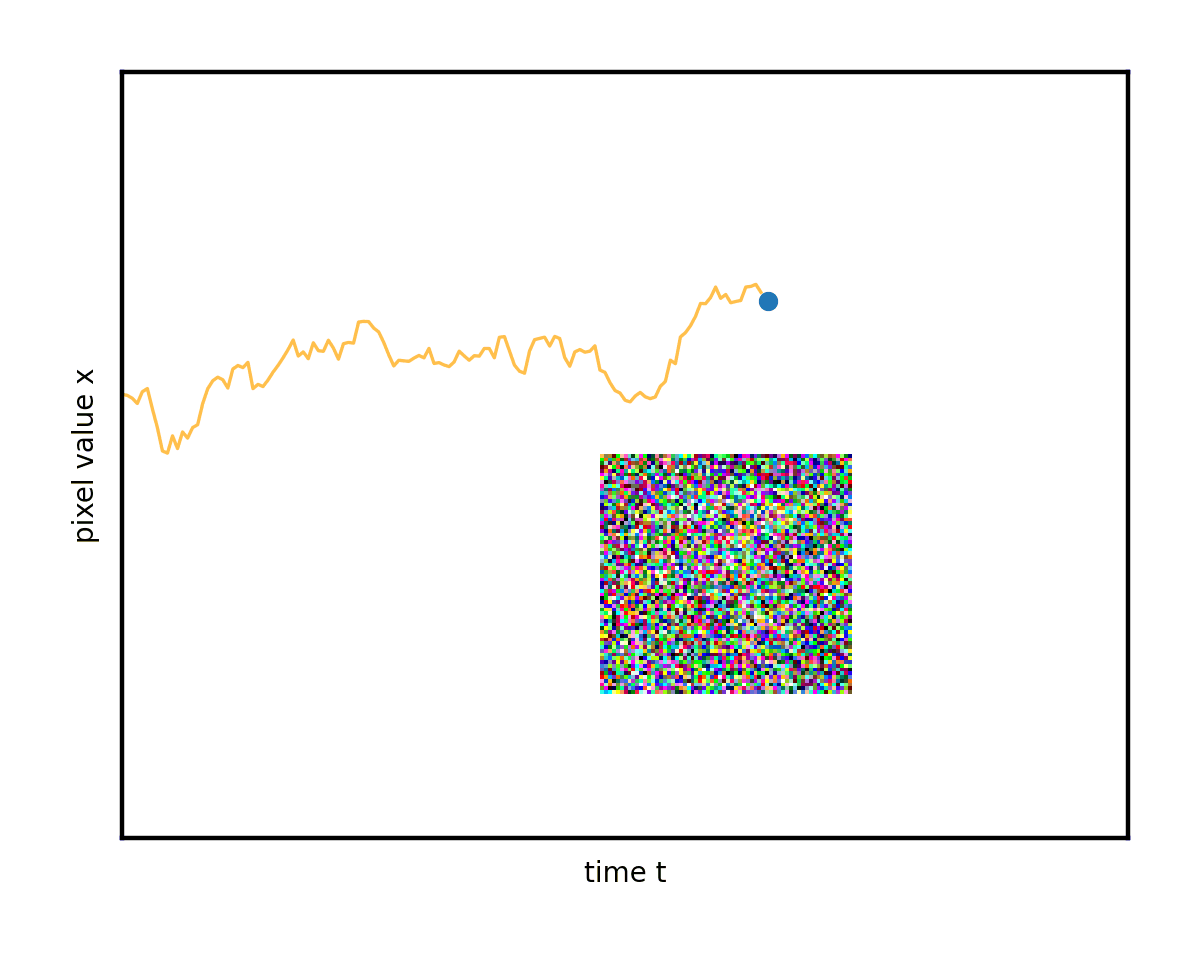
\includegraphics[width=0.85\textwidth]{frames/frame_012}}
%\only<14>{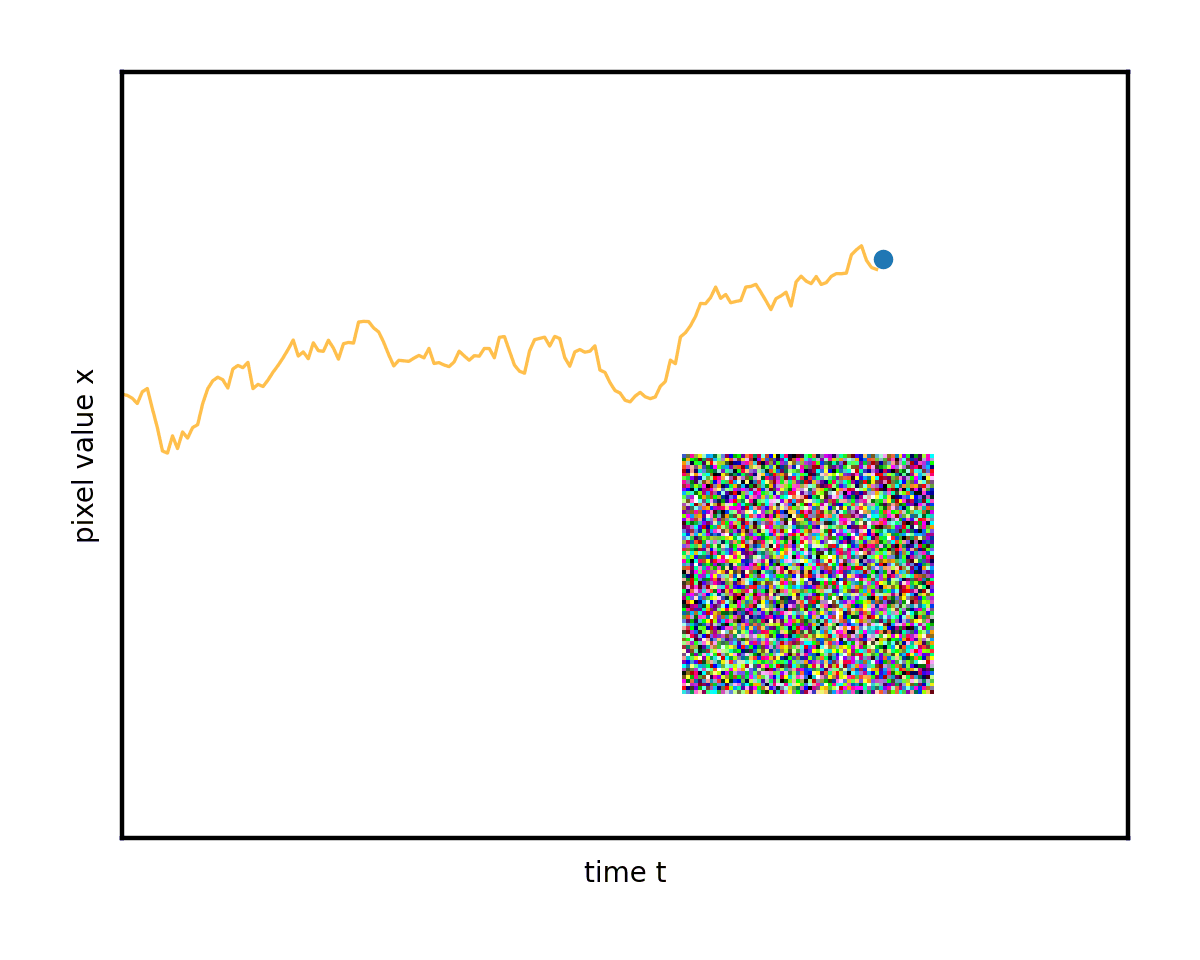
\includegraphics[width=0.85\textwidth]{frames/frame_013}}
%\only<15>{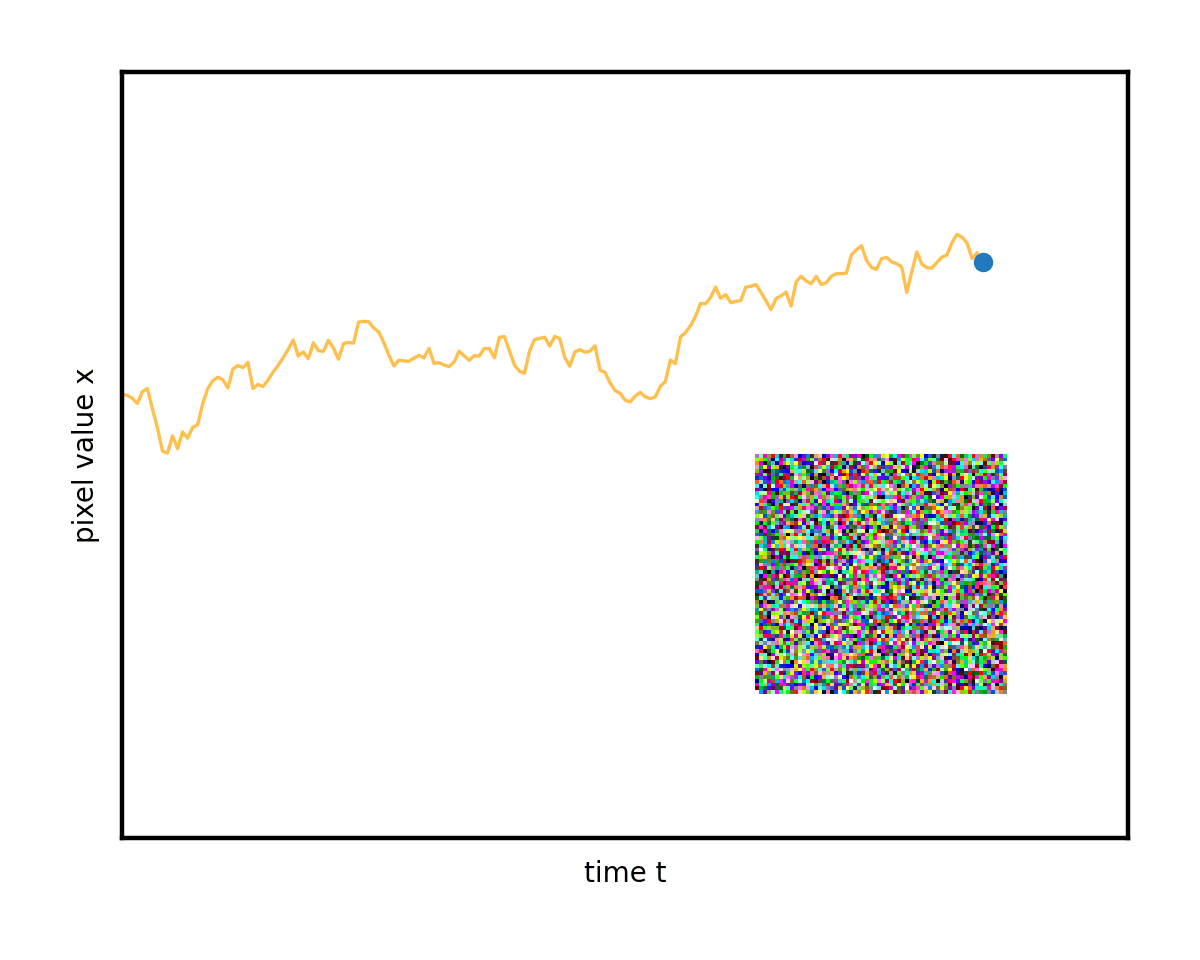
\includegraphics[width=0.85\textwidth]{frames/frame_014}}
%\only<16>{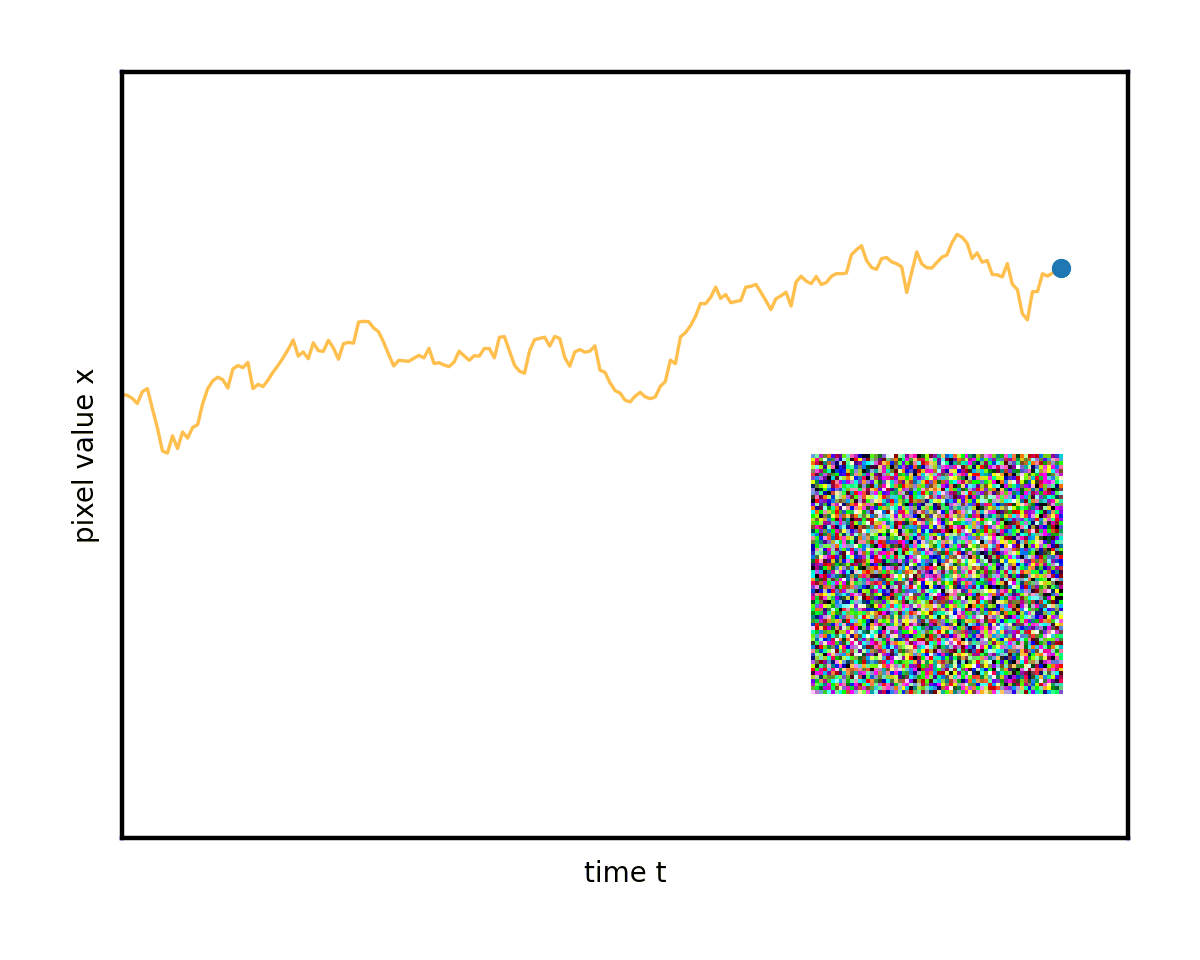
\includegraphics[width=0.85\textwidth]{frames/frame_015}}
%\only<17>{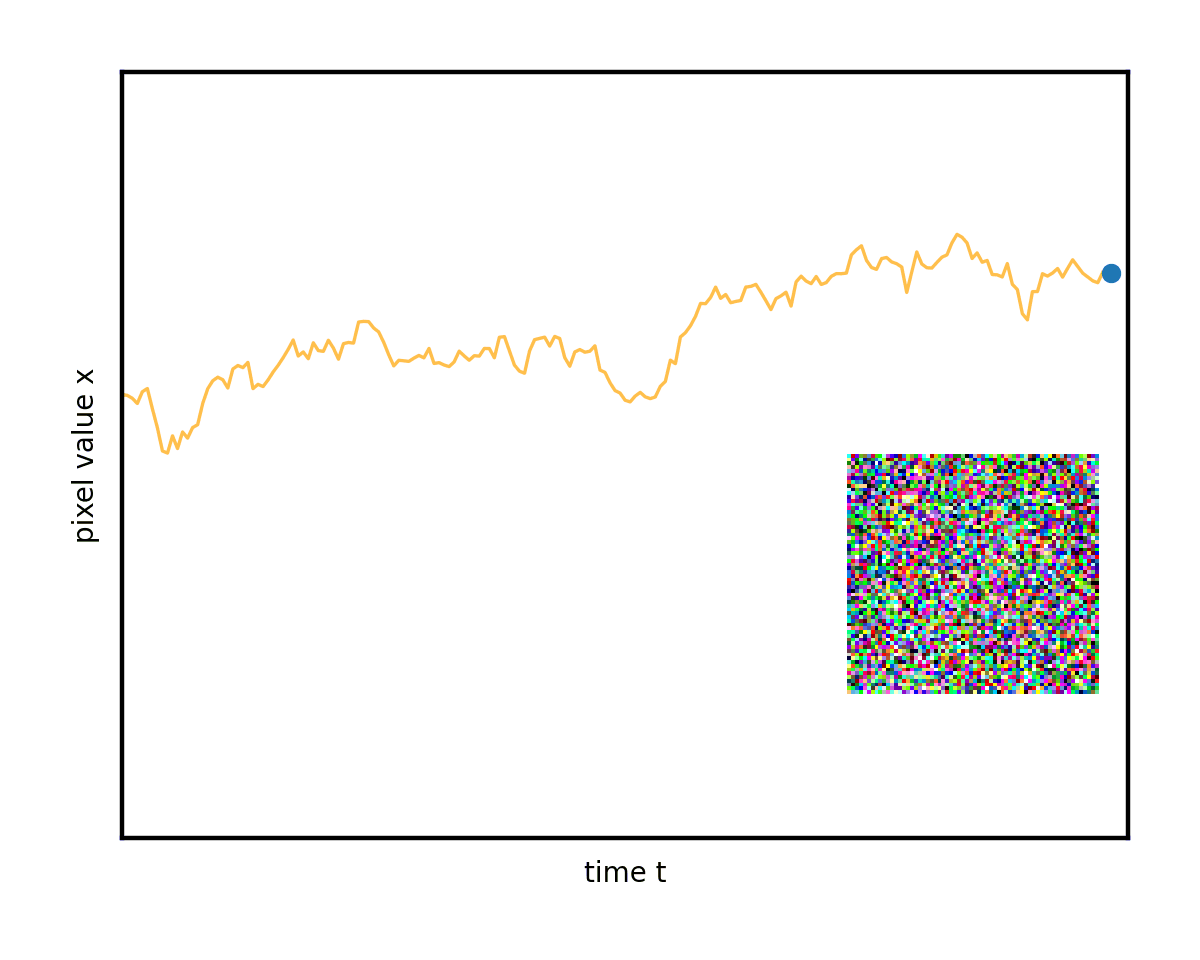
\includegraphics[width=0.85\textwidth]{frames/frame_016}}
%\only<18>{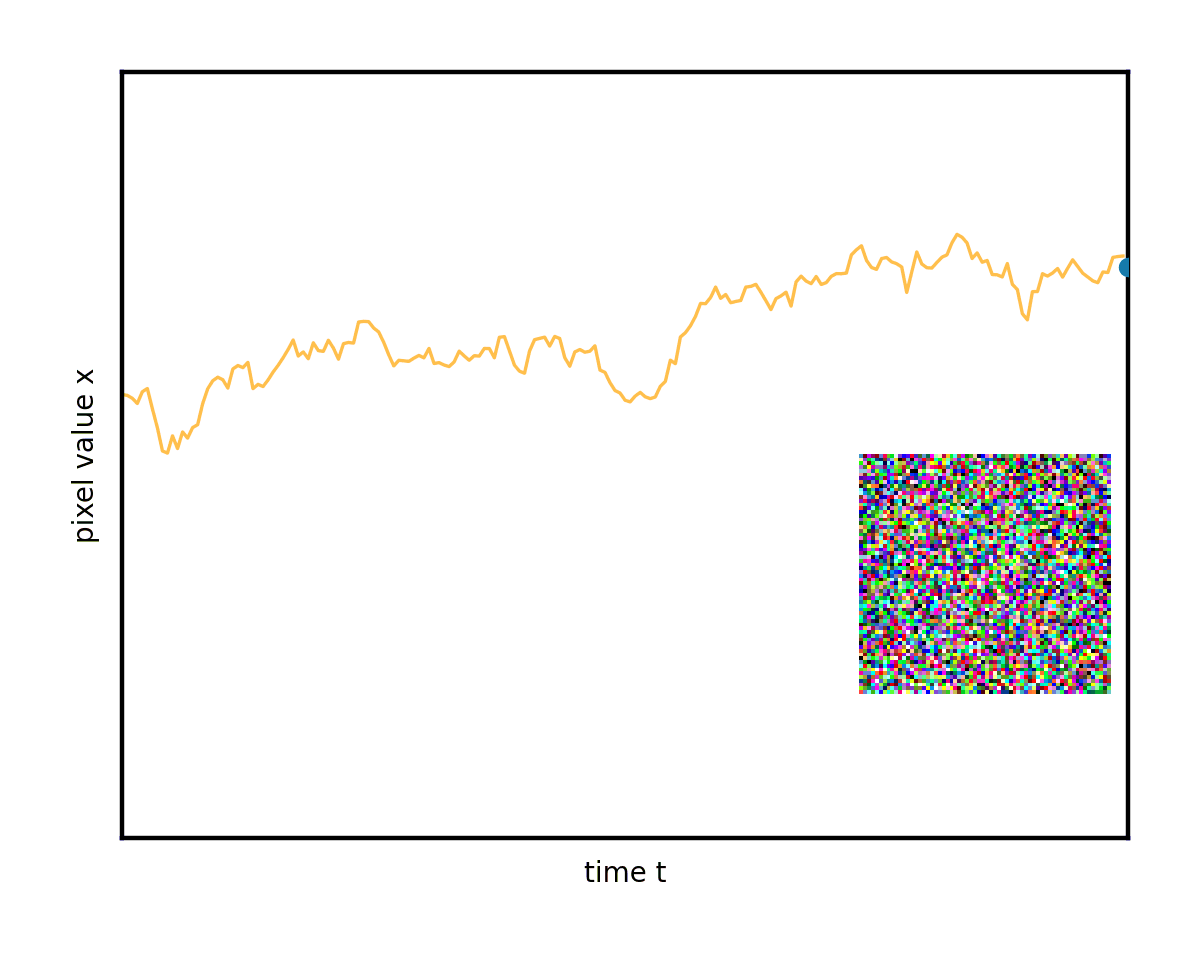
\includegraphics[width=0.85\textwidth]{frames/frame_017}}
%
%\end{frame}








\section{Mini-Lecture: Attention}

\begin{frame}[standout]
This is a slideshow version of the excellent video by \href{https://www.youtube.com/watch?v=eMlx5fFNoYc}{\alert{\underline{3Blue1Brown}}}.
\end{frame}


\begin{frame}{Modeling Goal}
\begin{figure} 
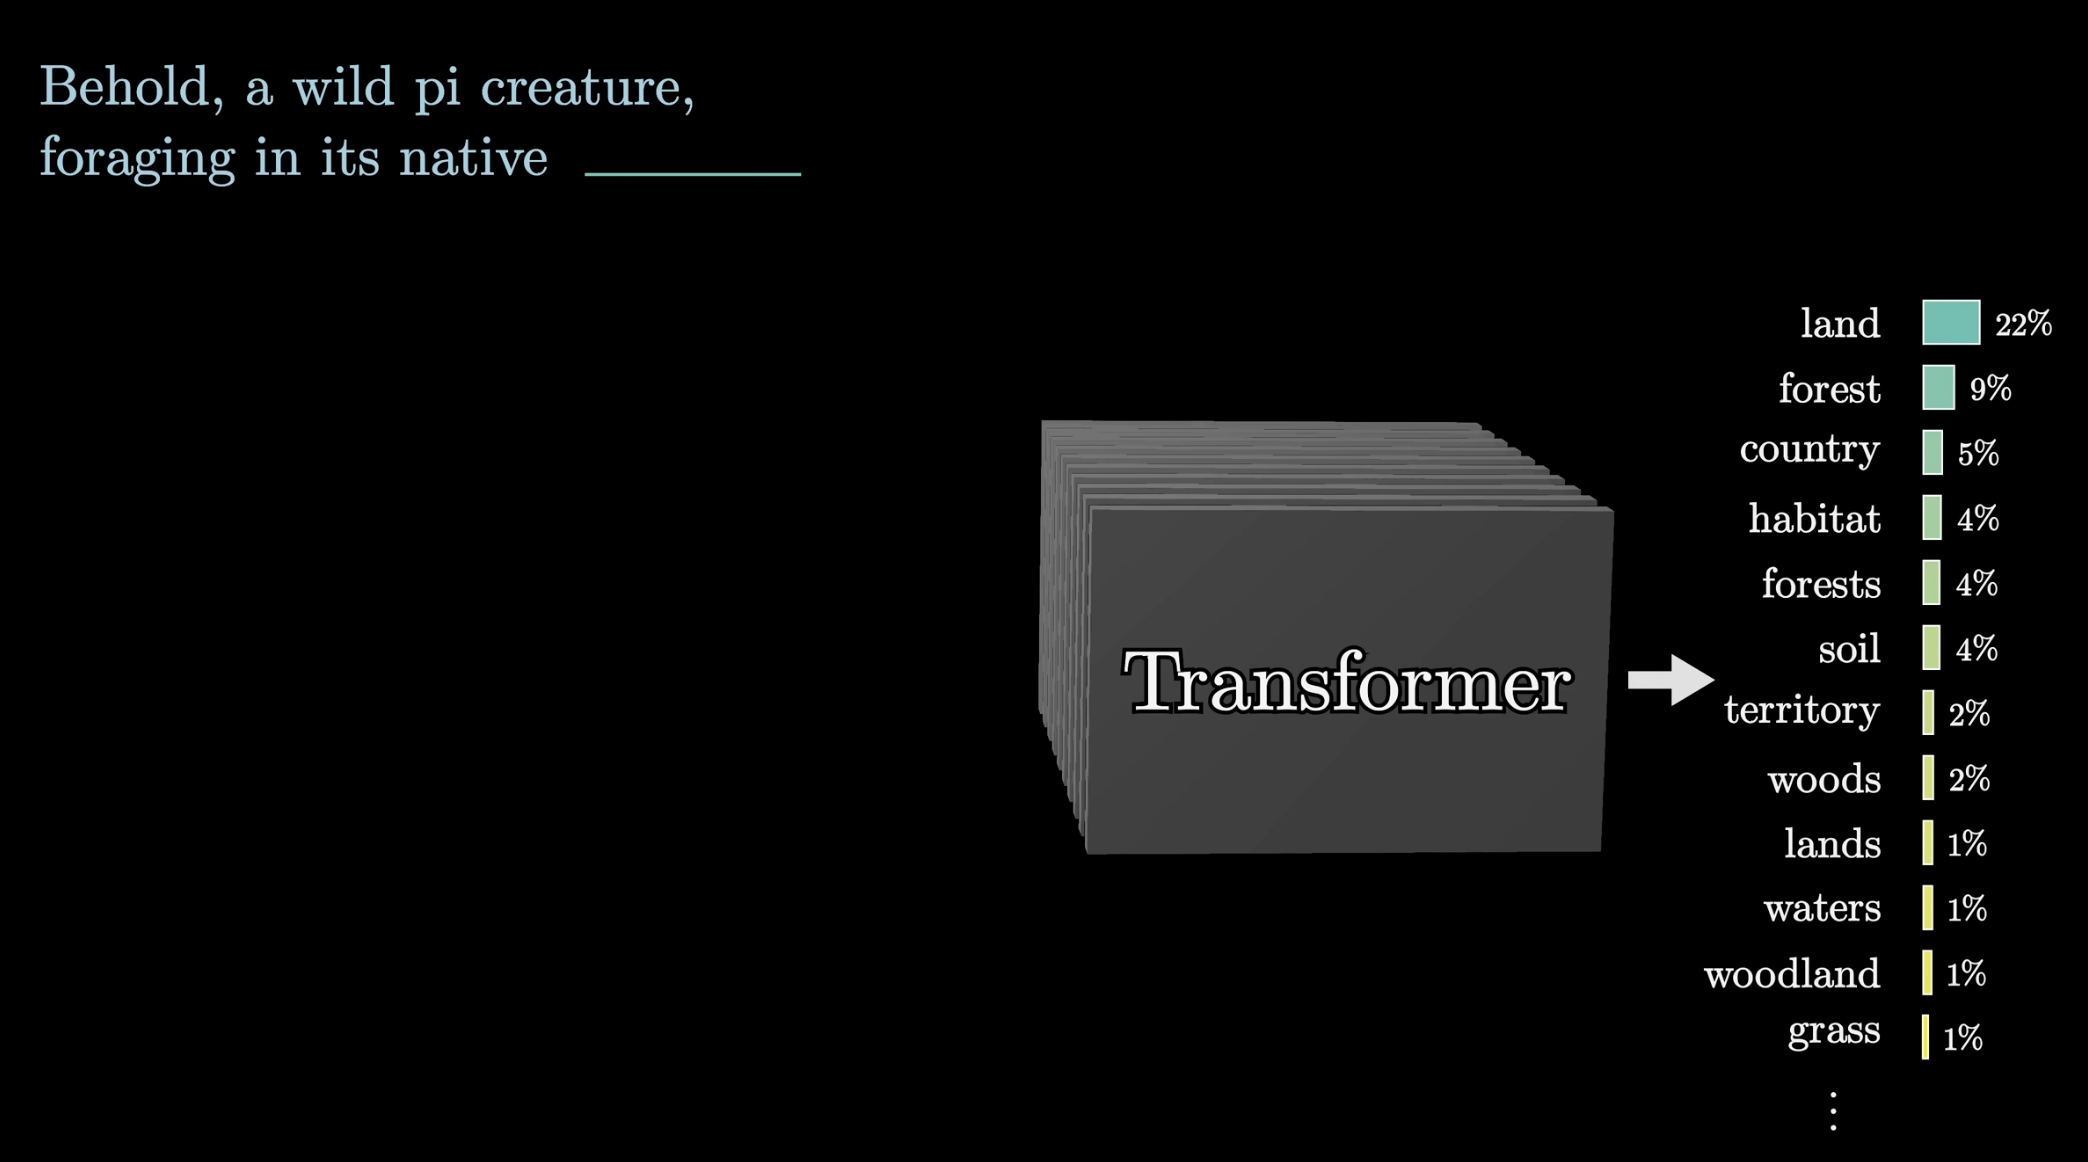
\includegraphics[width=1.0\textwidth]{images/goal} 
\end{figure}
\pause 
\begin{center}
The \alert{goal} is next word prediction.
\end{center}
\end{frame}

\begin{frame}{Tokenization}
\begin{figure} 
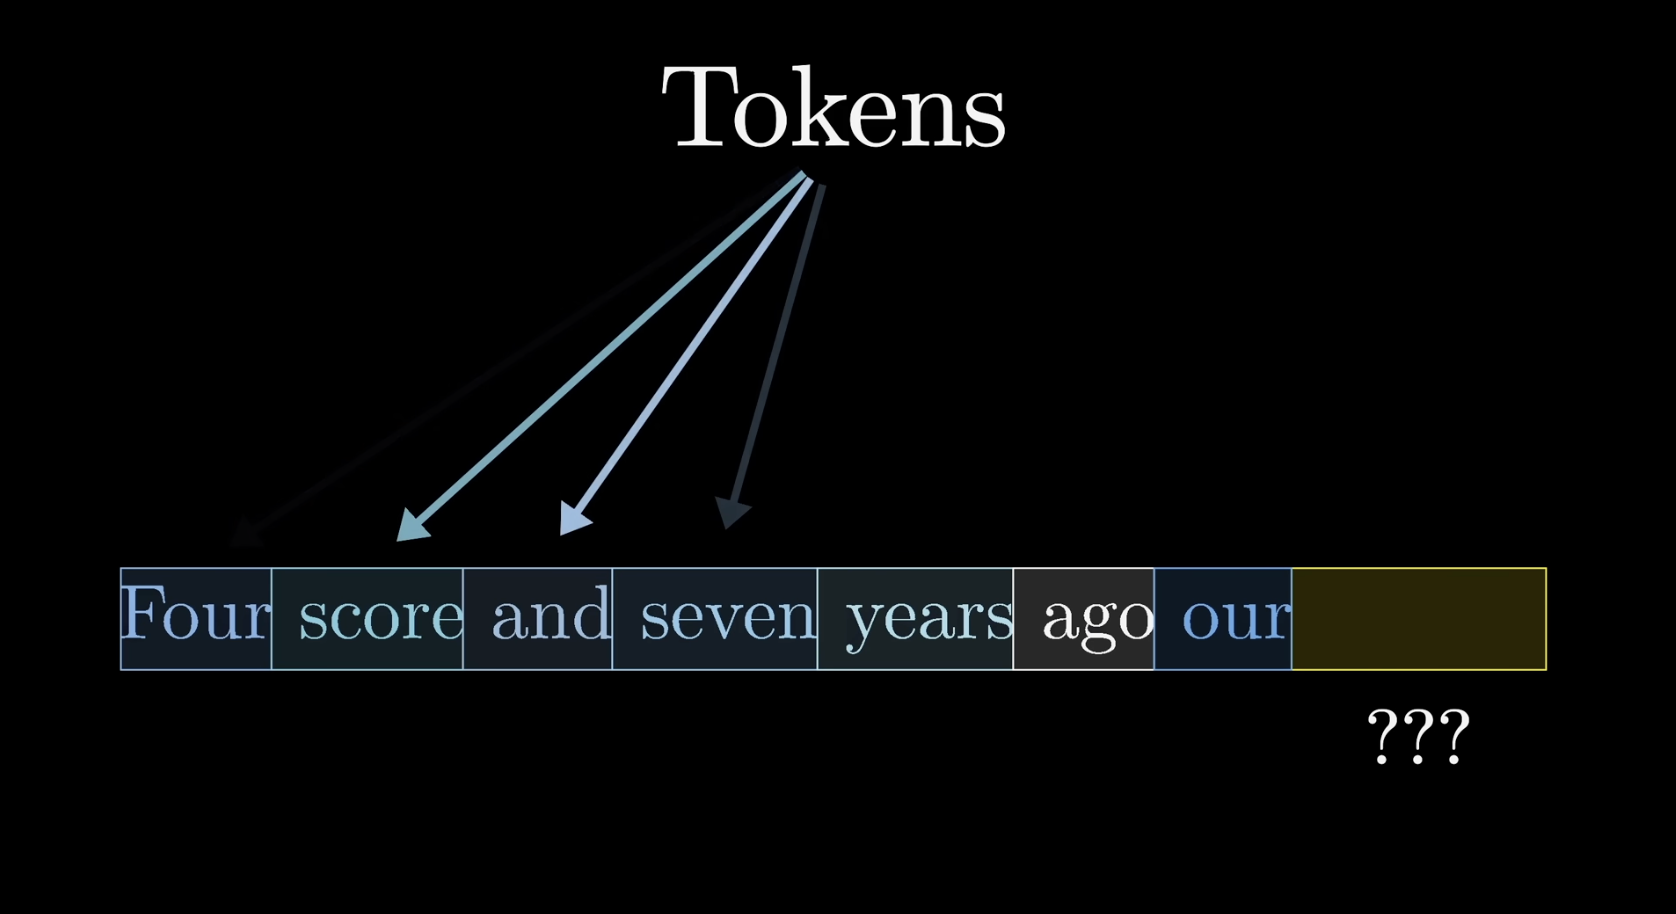
\includegraphics[width=1.0\textwidth]{images/tokens} 
\end{figure}
\pause 
\begin{center}
The input text is broken up into little pieces called \alert{tokens.}
\end{center}
\end{frame}

% TODO: Add in later once I understand it better.
%\begin{frame}{Tokenization}
%\begin{figure} 
%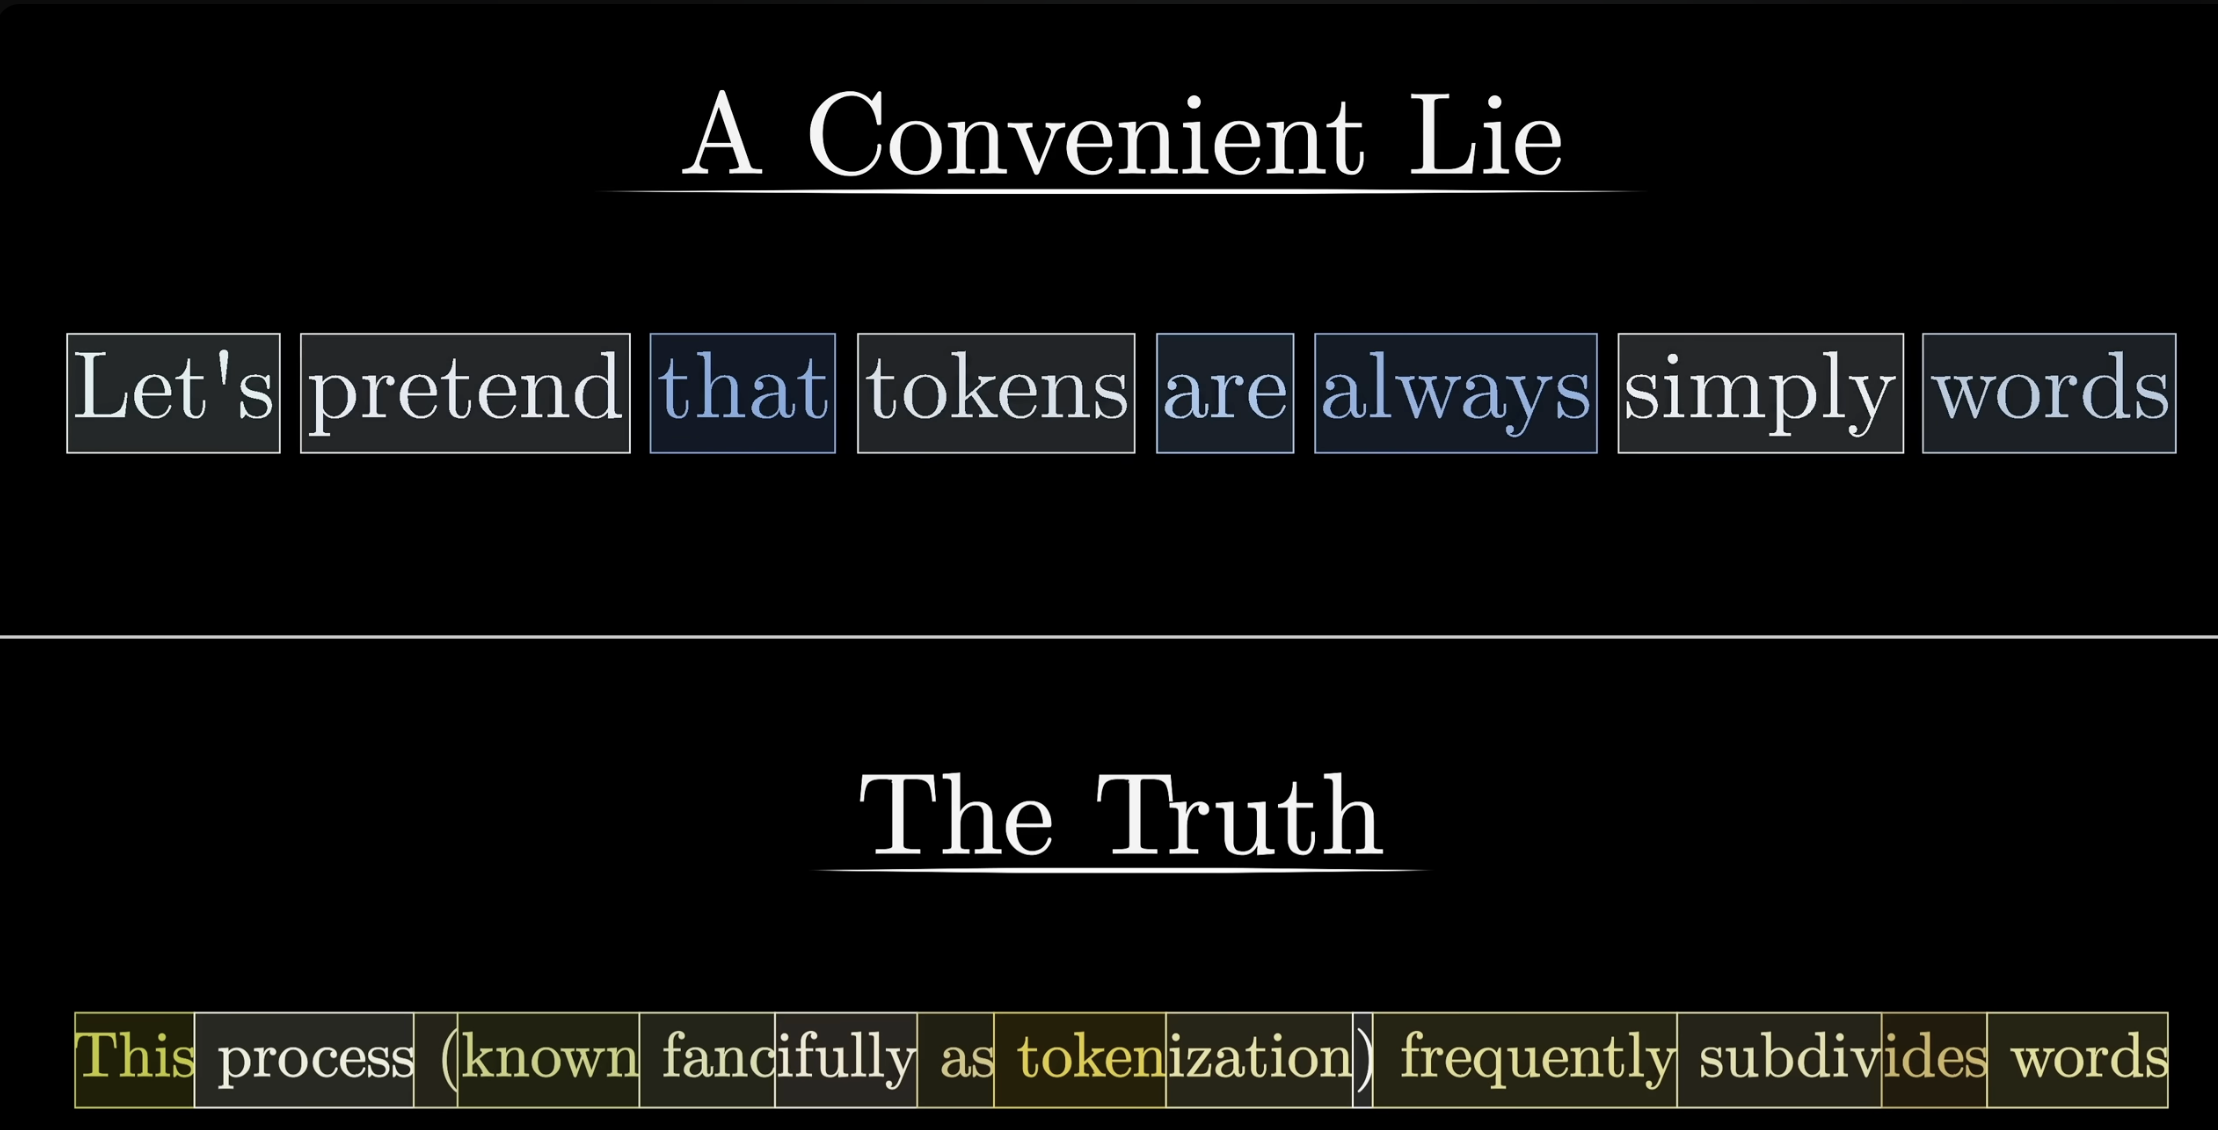
\includegraphics[width=1.0\textwidth]{images/tokens2} 
%\end{figure}
%\pause 
%\begin{center}
%For ease of exposition, we'll assume that tokens are words.
%\end{center}
%
%\end{frame}



\begin{frame}{Embeddings}
\begin{figure} 
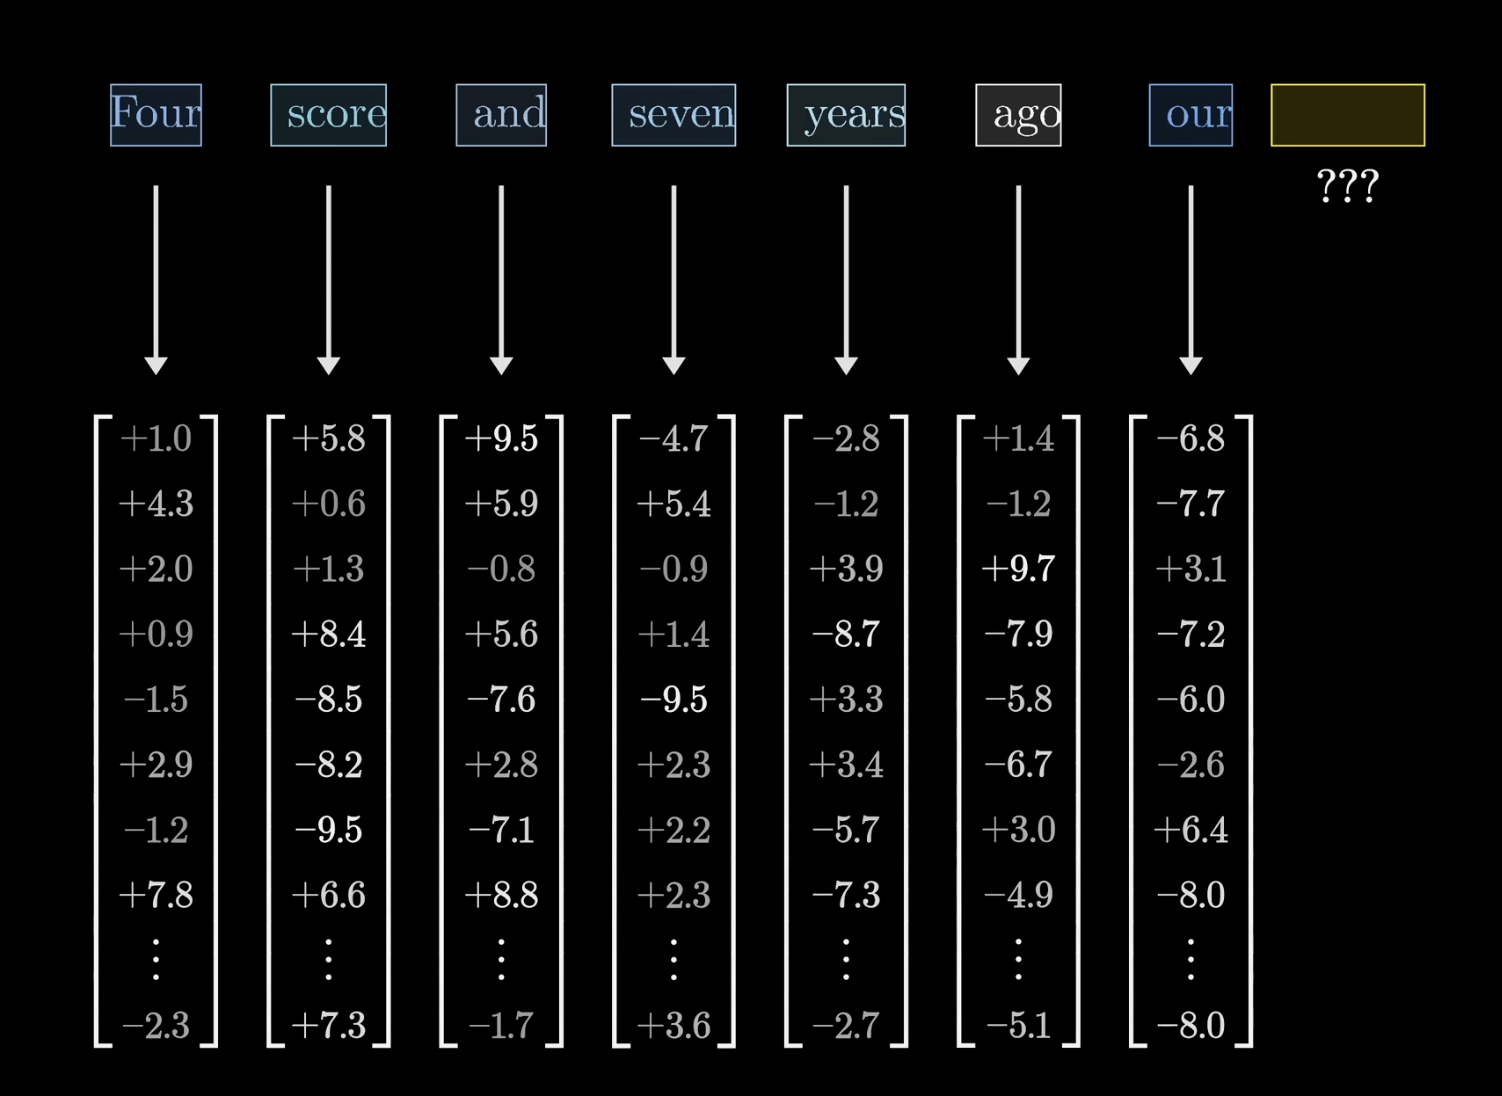
\includegraphics[width=0.8\textwidth]{images/embedding} 
\end{figure}
\pause 
\begin{center}
\textbf{First step}:  We associate each word with a high-dimensional vector, called its \alert{embedding}.
\end{center}
\end{frame}

\begin{frame}{Embeddings}
\begin{figure} 
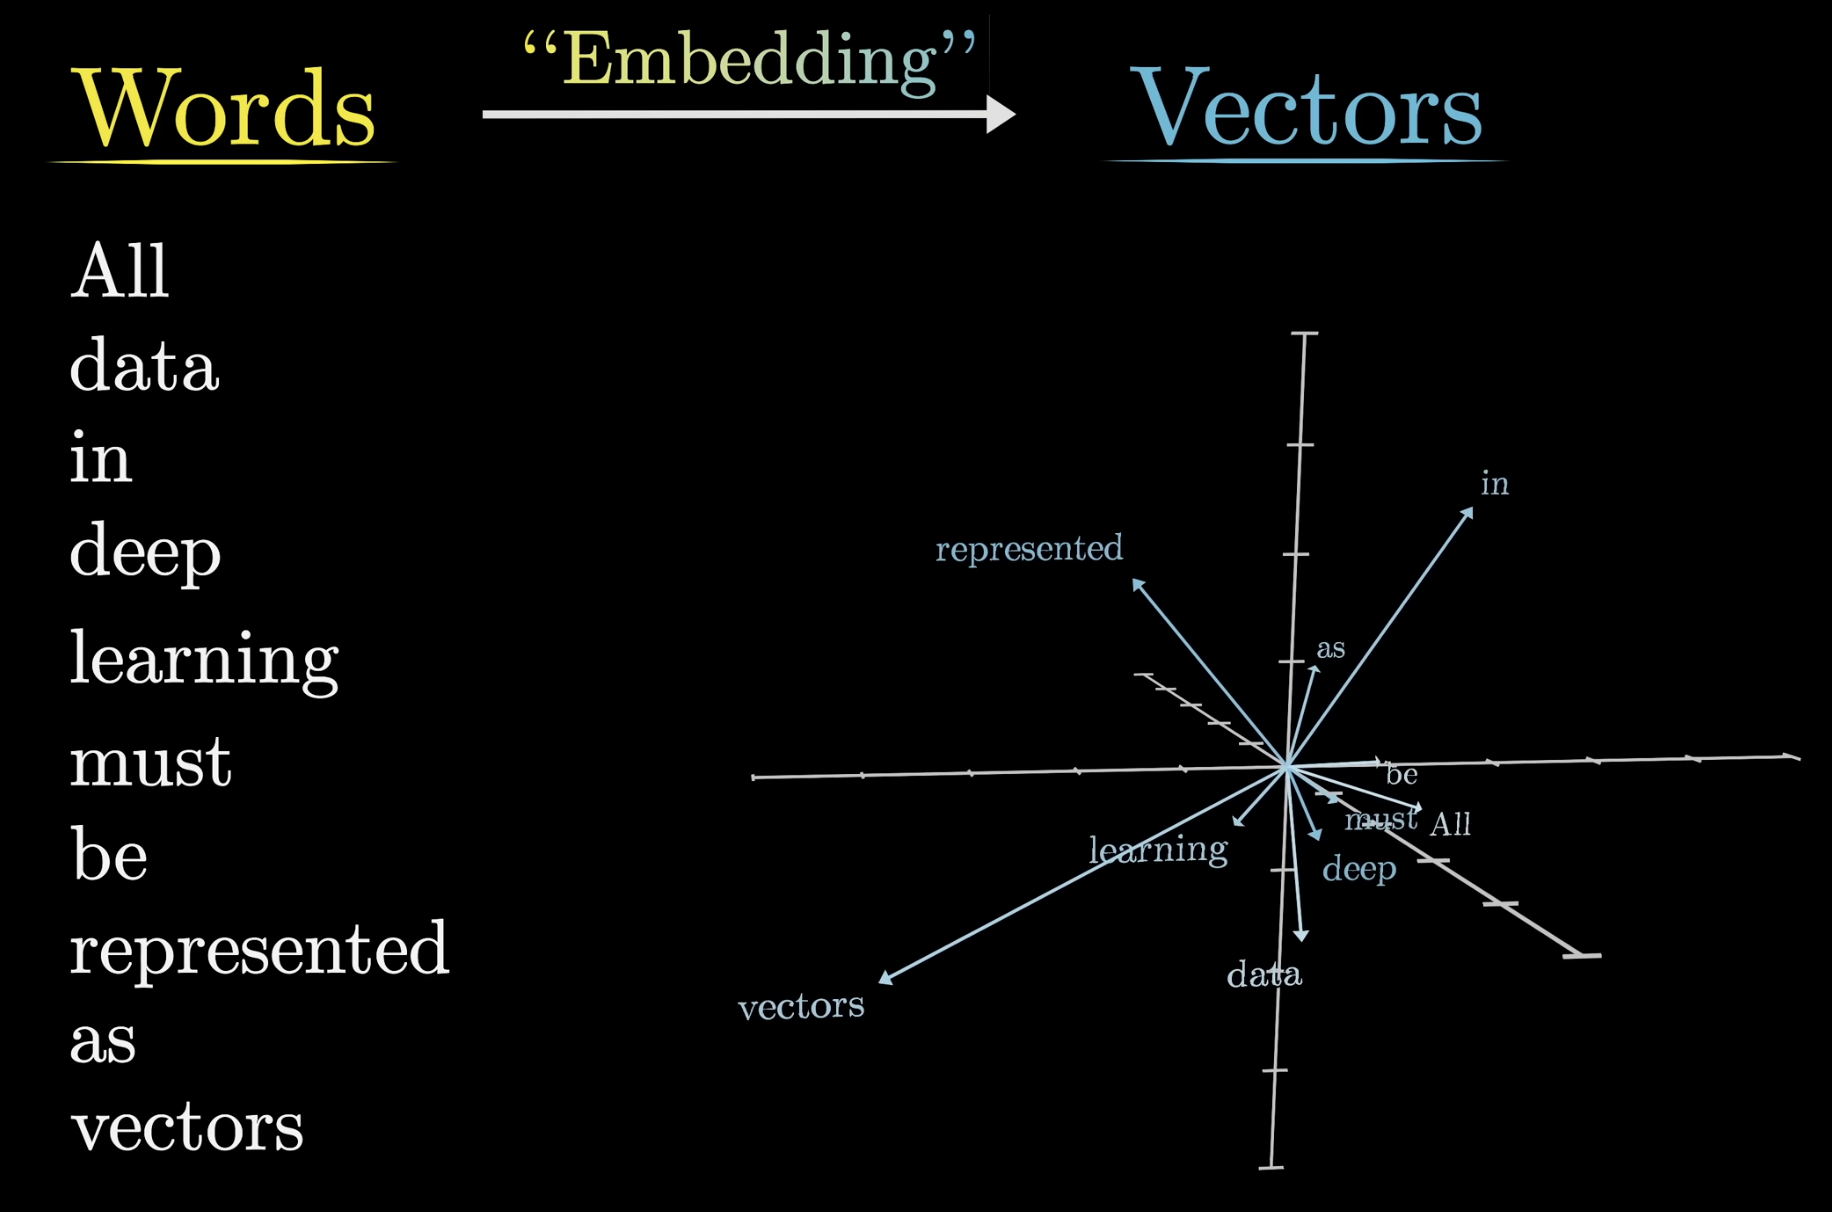
\includegraphics[width=0.8\textwidth]{images/directions} 
\end{figure}
\pause 
\begin{center}
Directions in this high-dimensional space can correspond to \alert{semantic meaning}.
\end{center}
\end{frame}

\begin{frame}{Embeddings}

\begin{center}
\only<1-2>{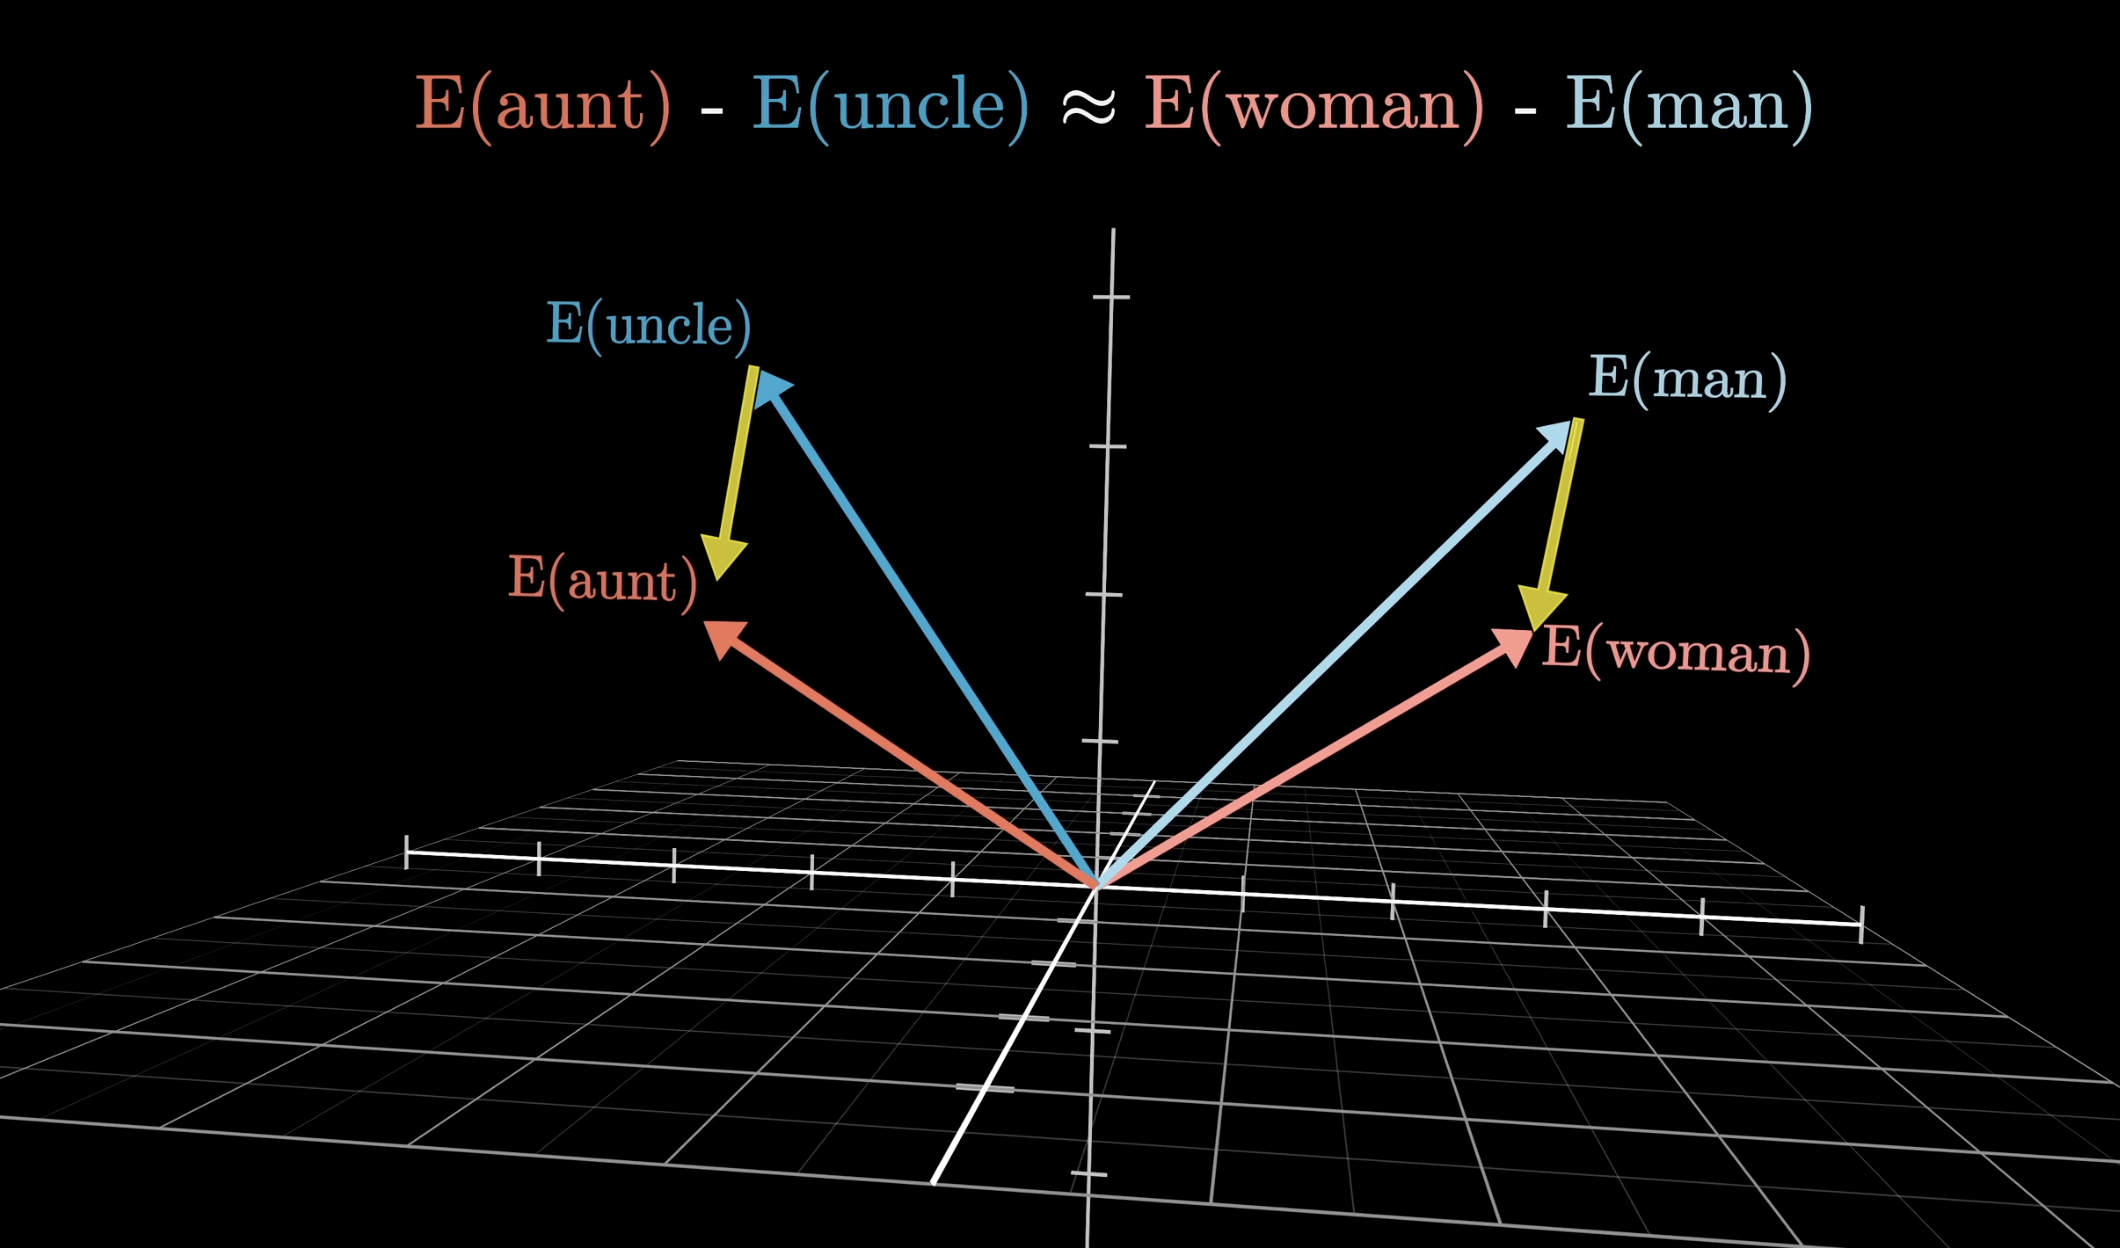
\includegraphics[width=0.85\textwidth]{images/gender1}}
\only<3>{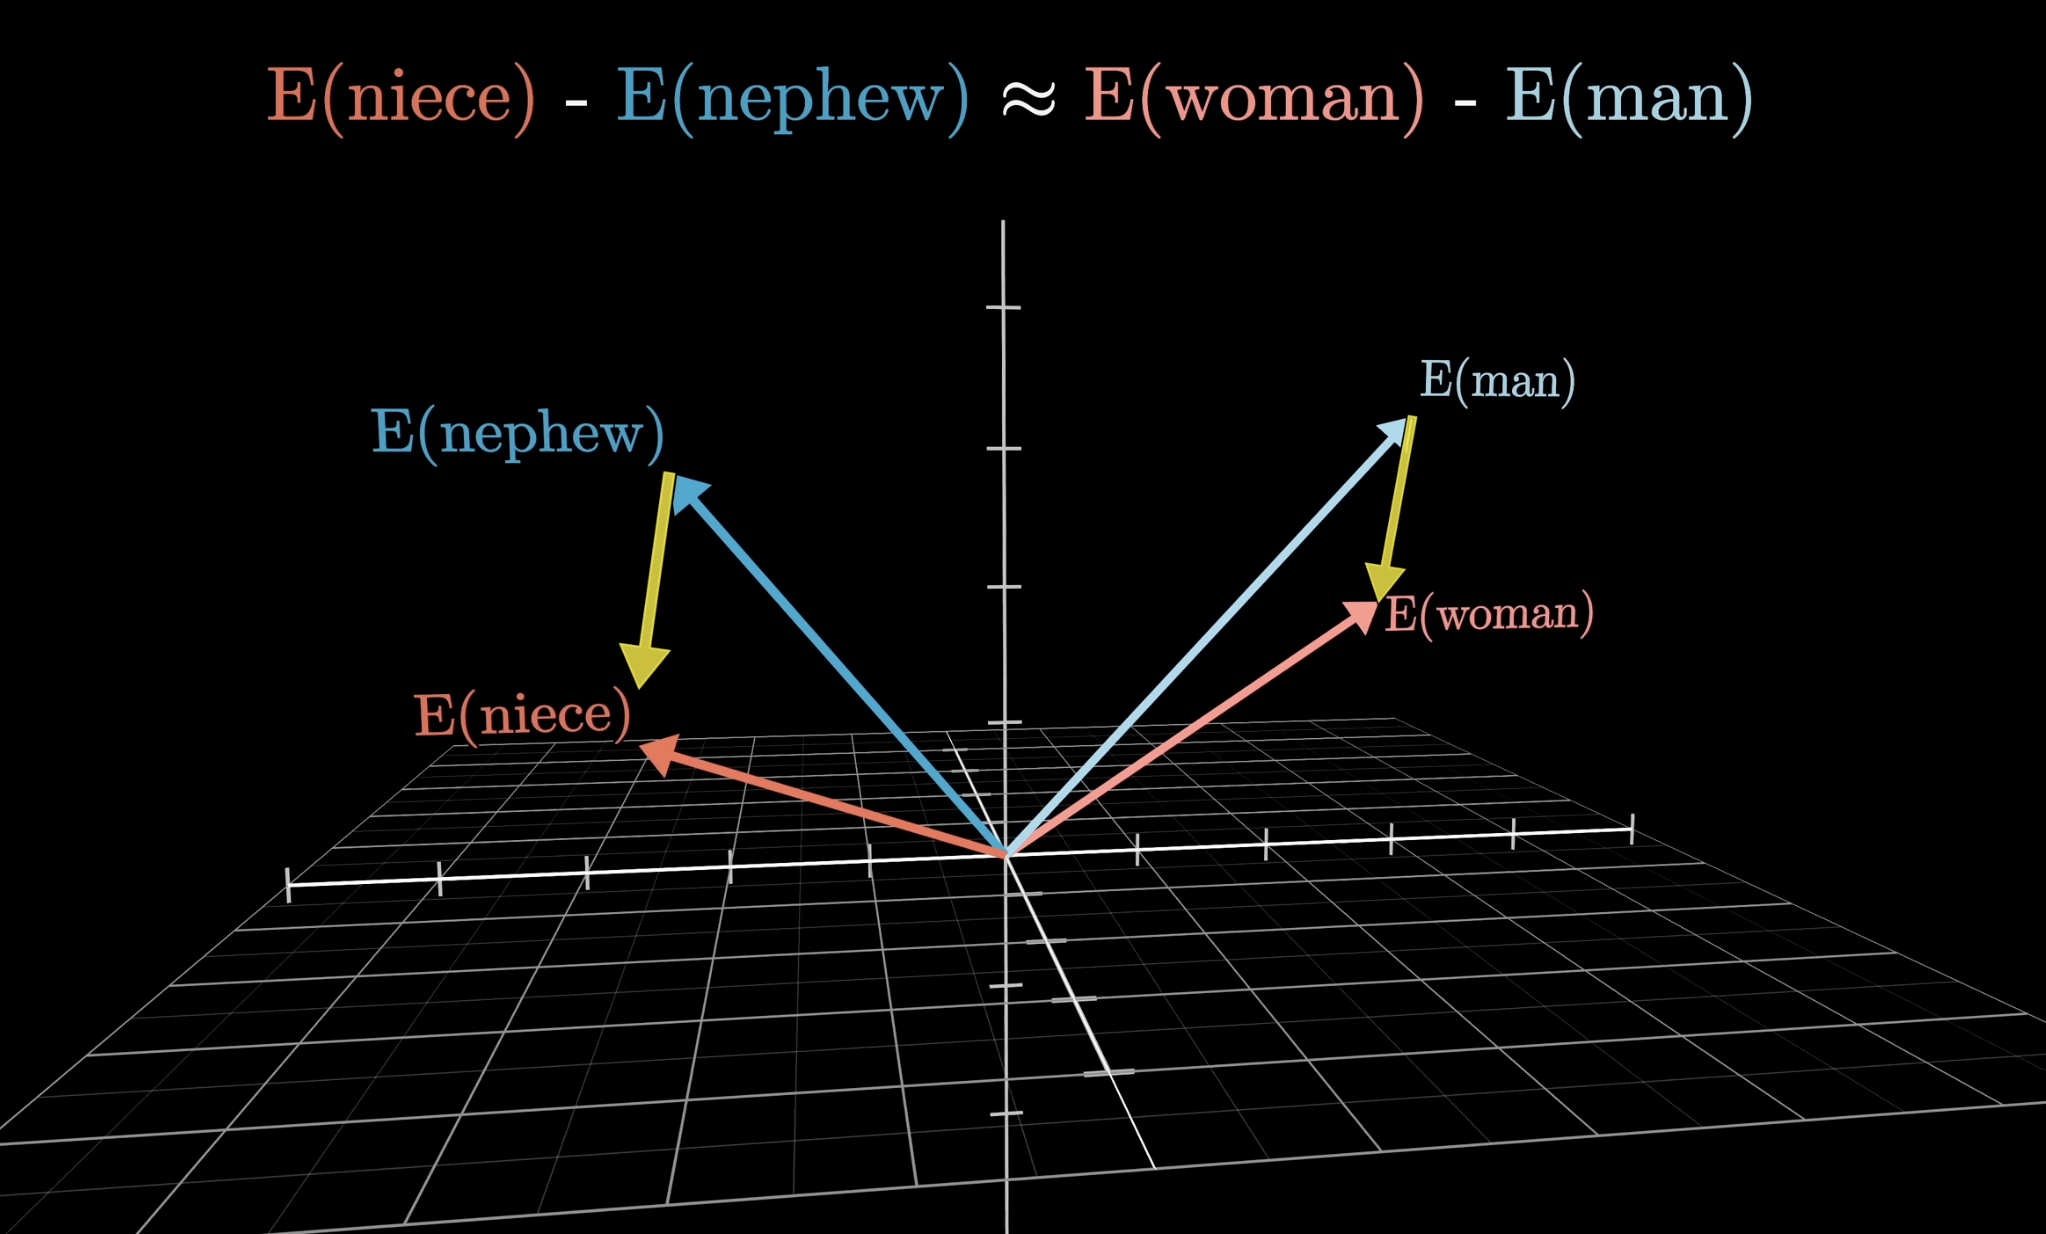
\includegraphics[width=0.85\textwidth]{images/gender2}}
\only<4>{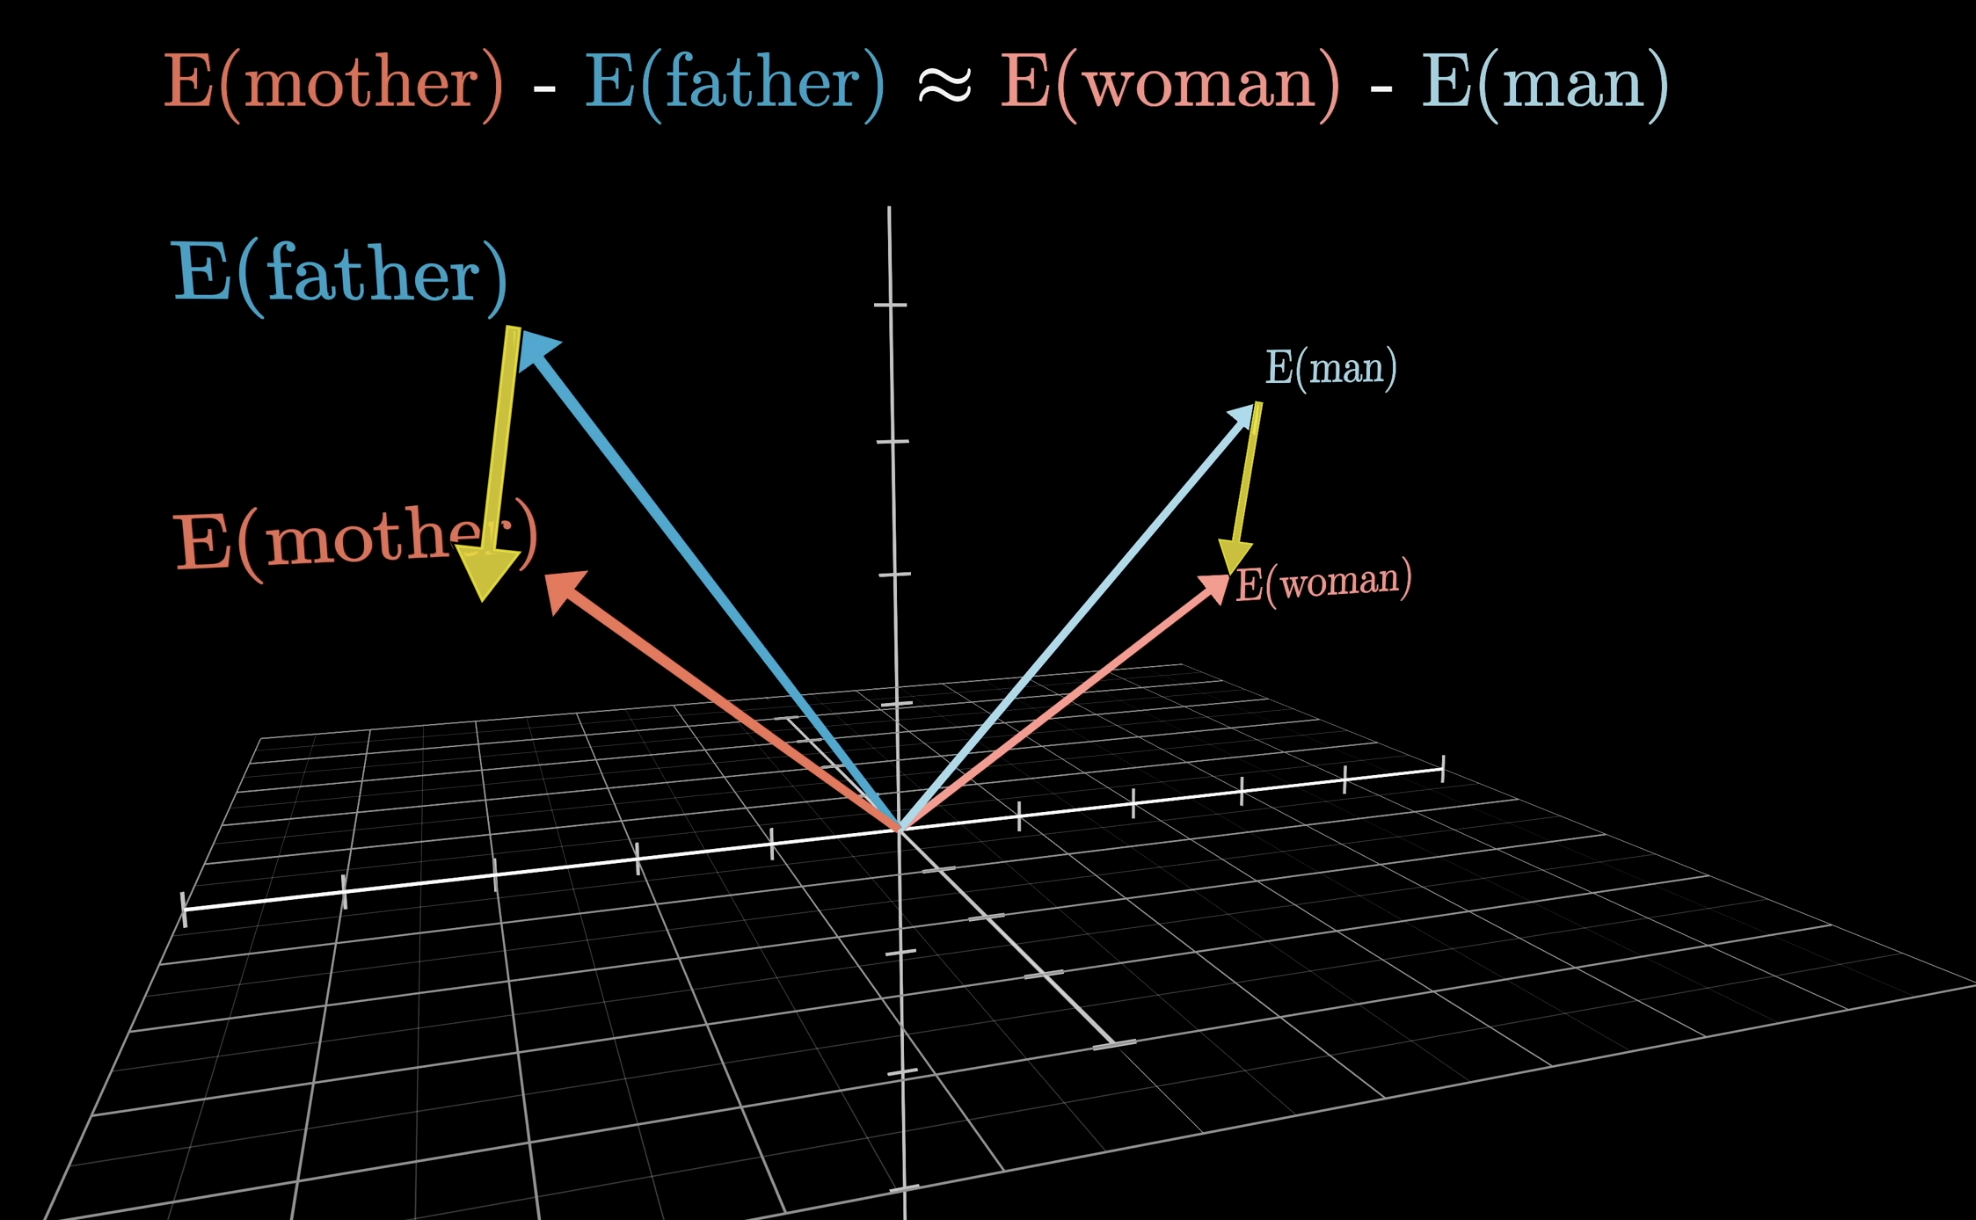
\includegraphics[width=0.85\textwidth]{images/gender3}}
\only<5>{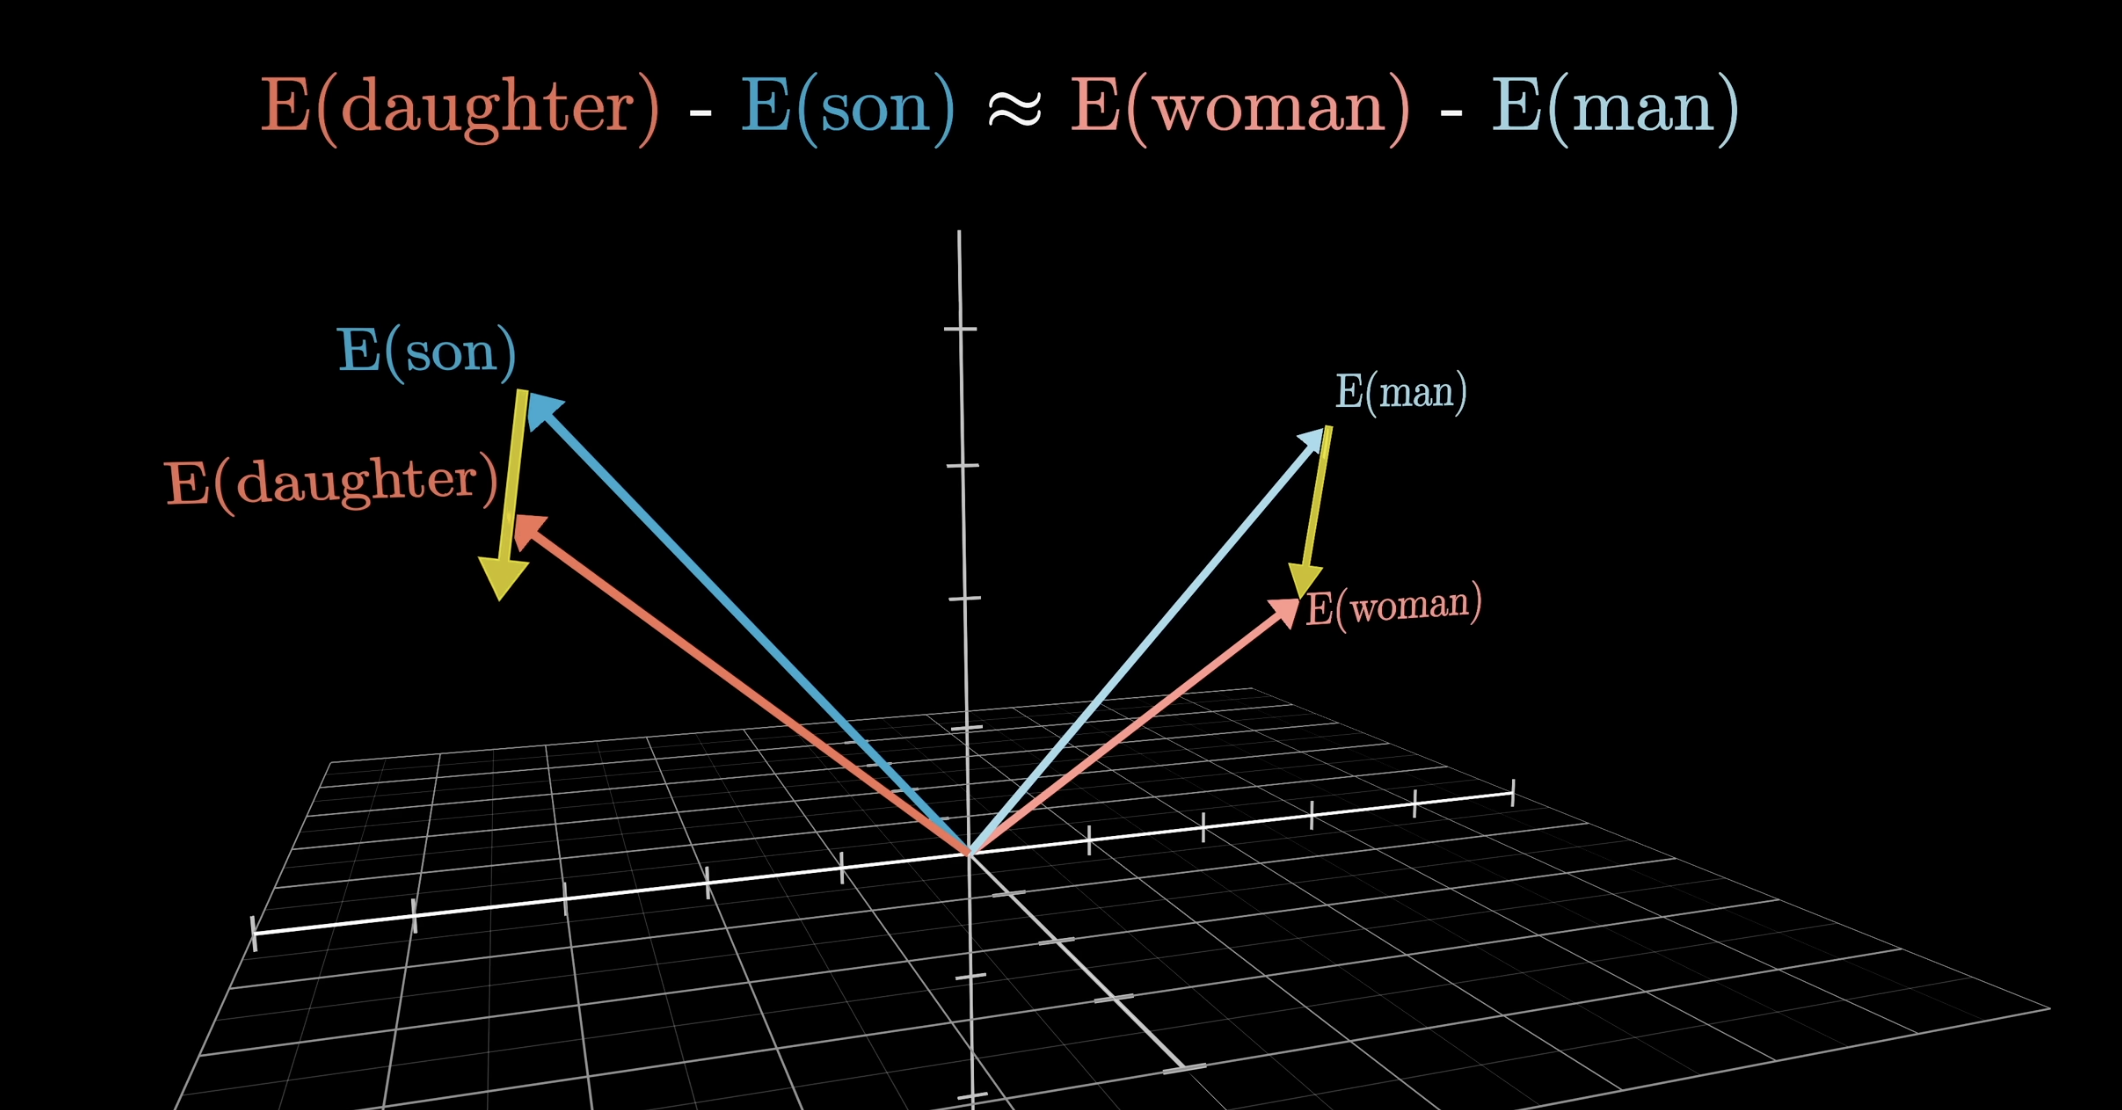
\includegraphics[width=0.85\textwidth]{images/gender4}}

\only<1->{
\textbf{Example}:  Directions in this high-dimensional space can correspond to gender.
} 
\only<2->{Adding a fixed step can take you from a masculine noun to the corresponding feminine noun.
}
\end{center}
\end{frame}


\begin{frame}{Embeddings}
\begin{figure} 
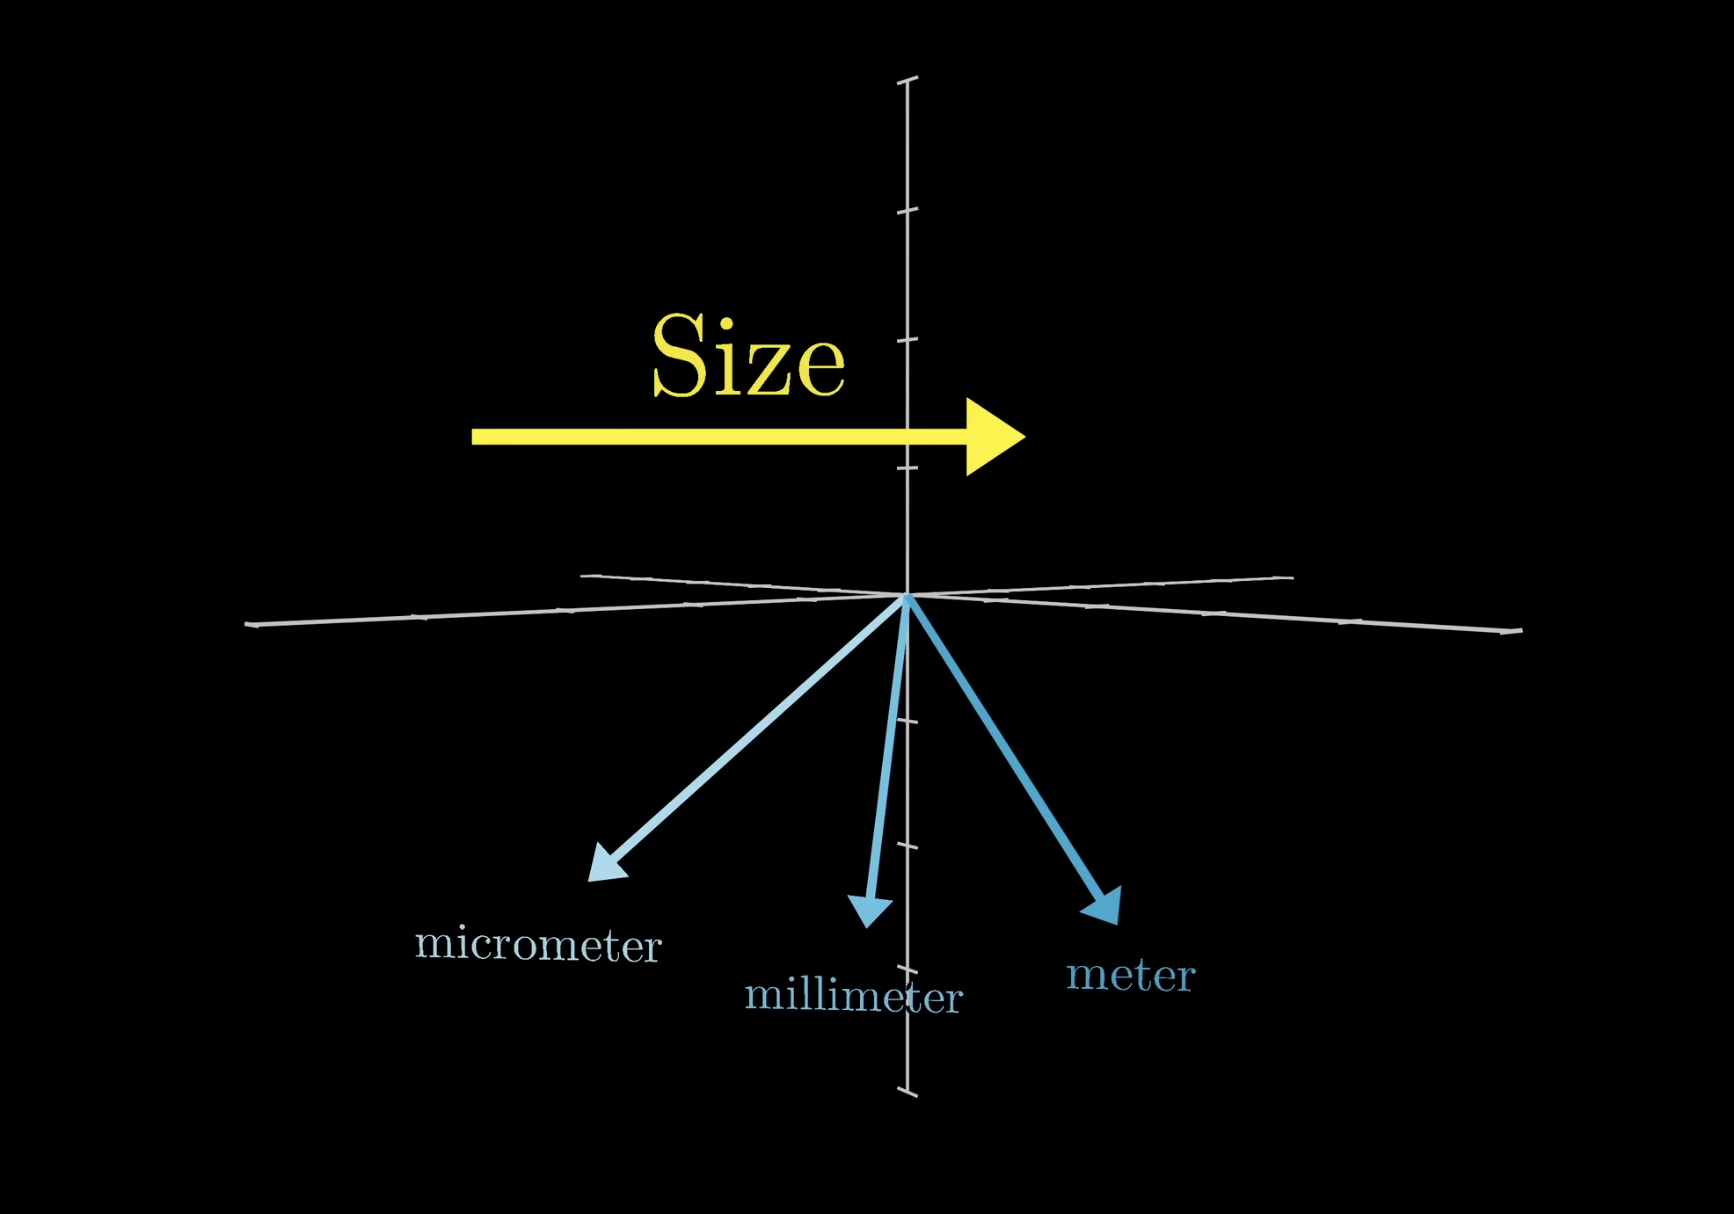
\includegraphics[width=0.8\textwidth]{images/other_directions} 
\end{figure}
\pause 
\begin{center}
Other directions can correspond to other aspects of a word's meaning.
\end{center}
\end{frame}


\begin{frame}{Aim of transformer}

\begin{center}
\only<1>{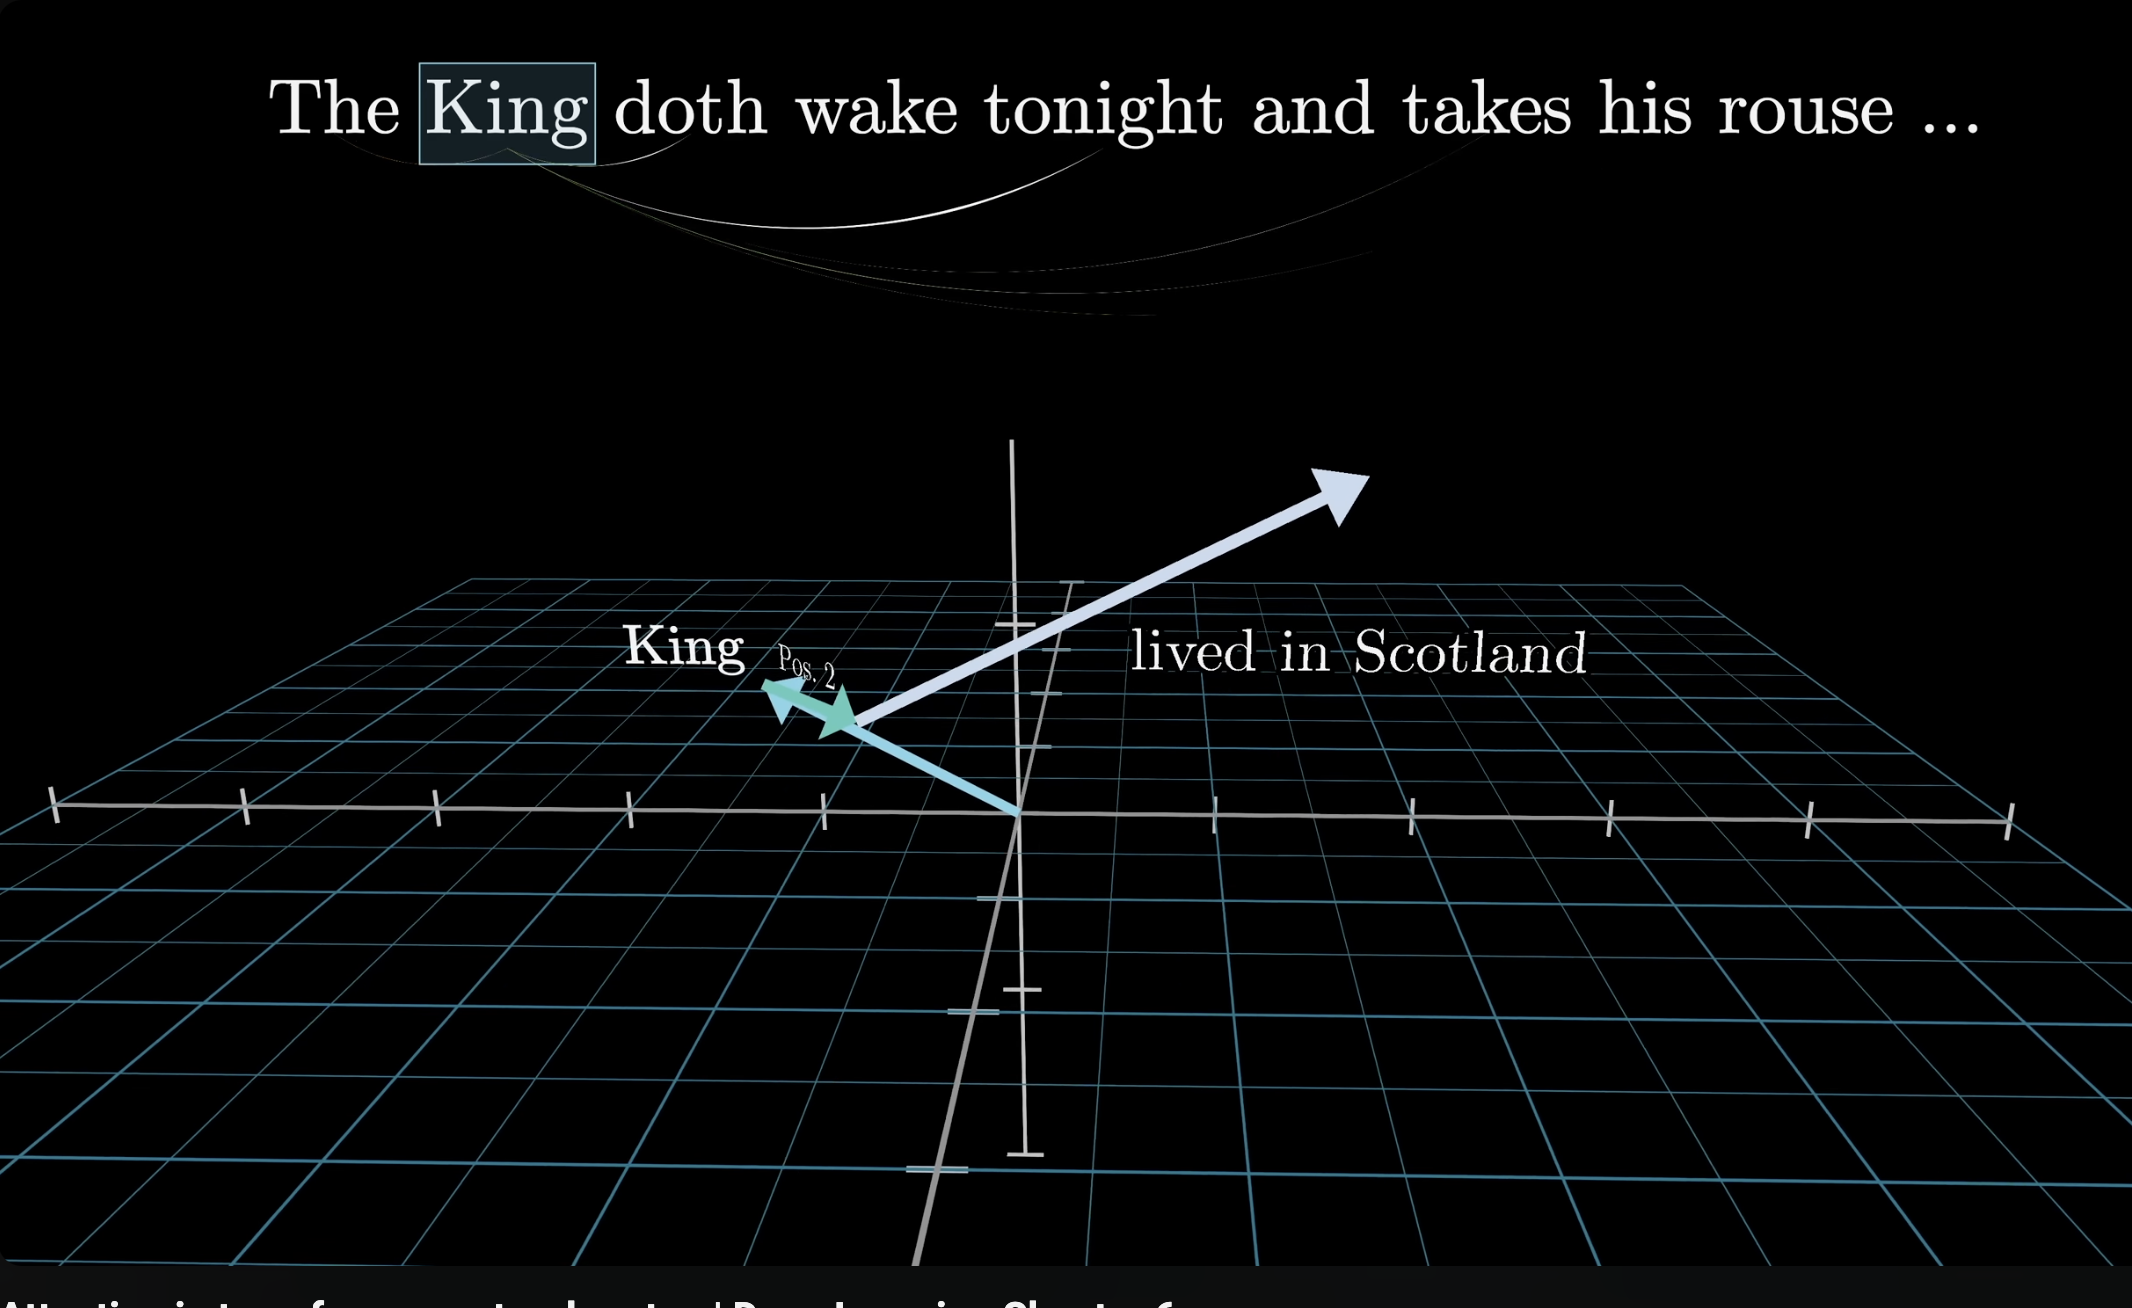
\includegraphics[width=0.85\textwidth]{images/adjust1}}
\only<2>{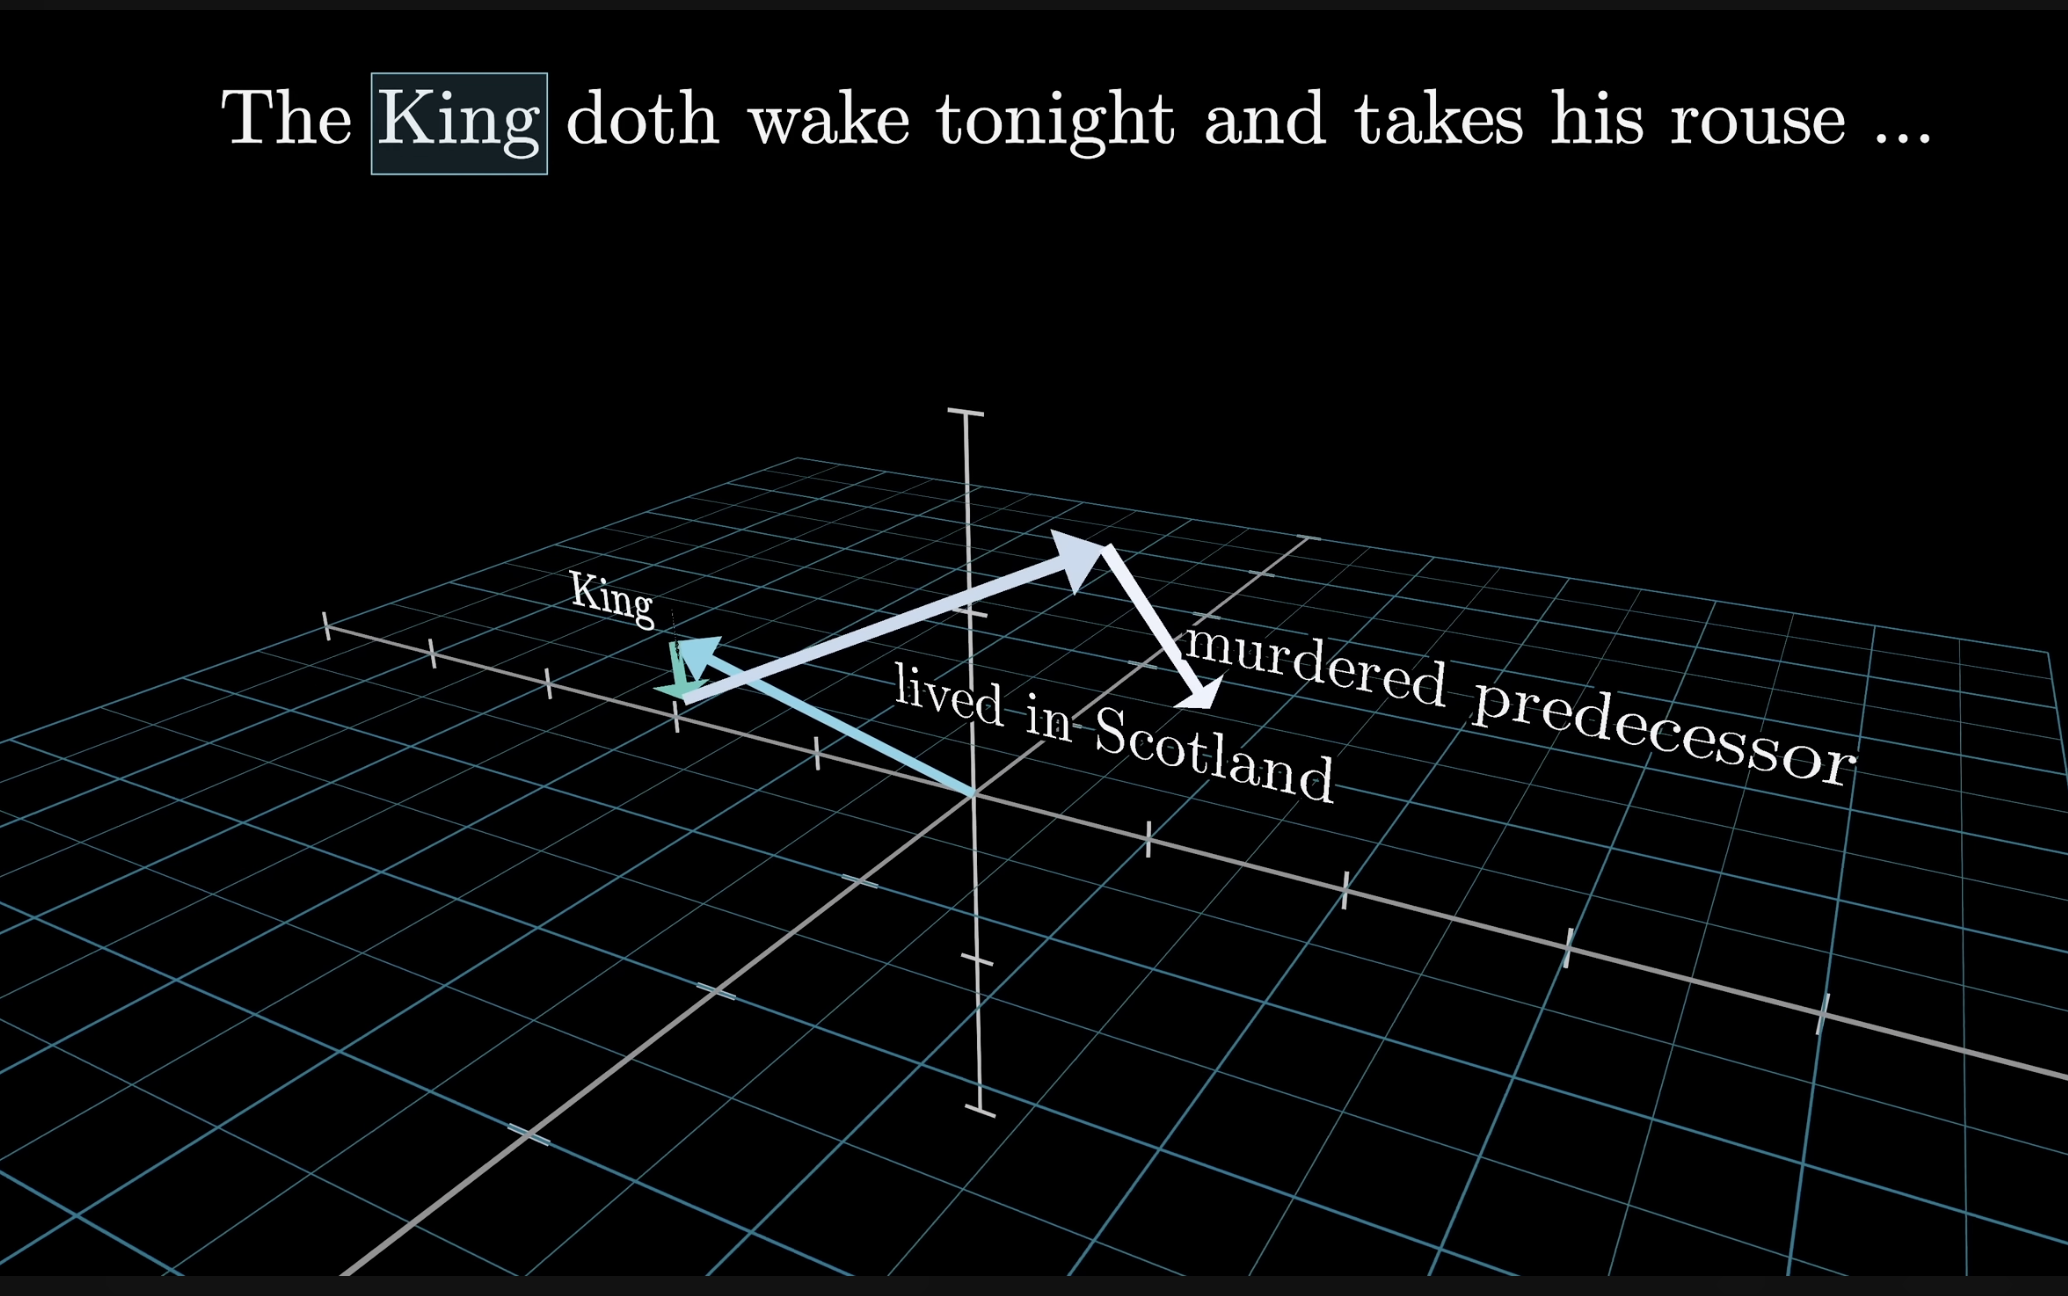
\includegraphics[width=0.85\textwidth]{images/adjust2}}
\only<3>{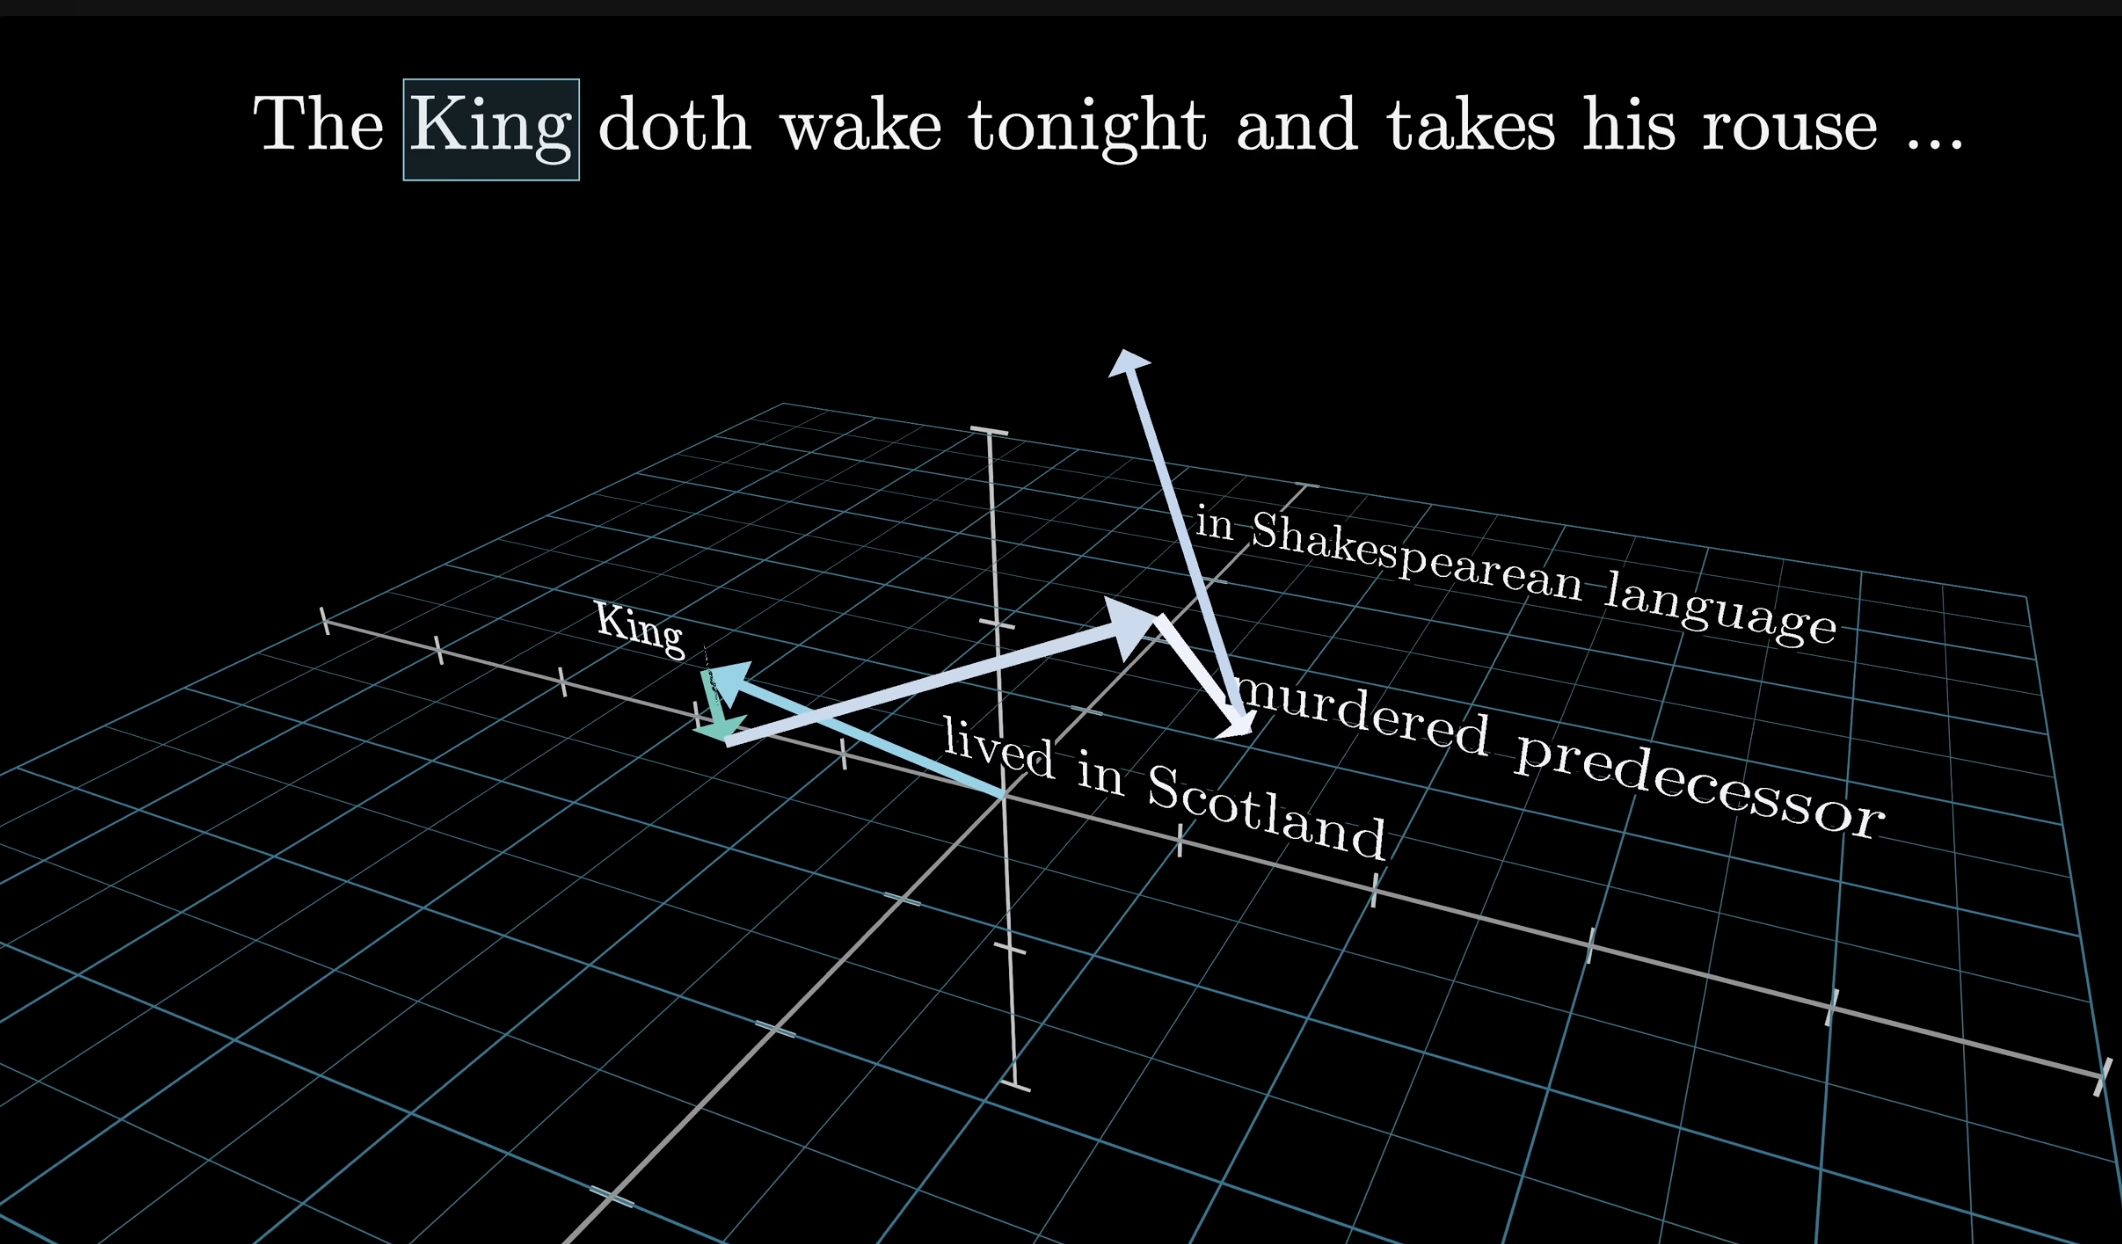
\includegraphics[width=0.85\textwidth]{images/adjust3}}

\only<1->{
We want to progressively adjust these embeddings to encode not just an individual word, but richer contextual meaning.  
} 
\end{center}

\end{frame}



\begin{frame}{Aim of transformer}
\begin{figure} 
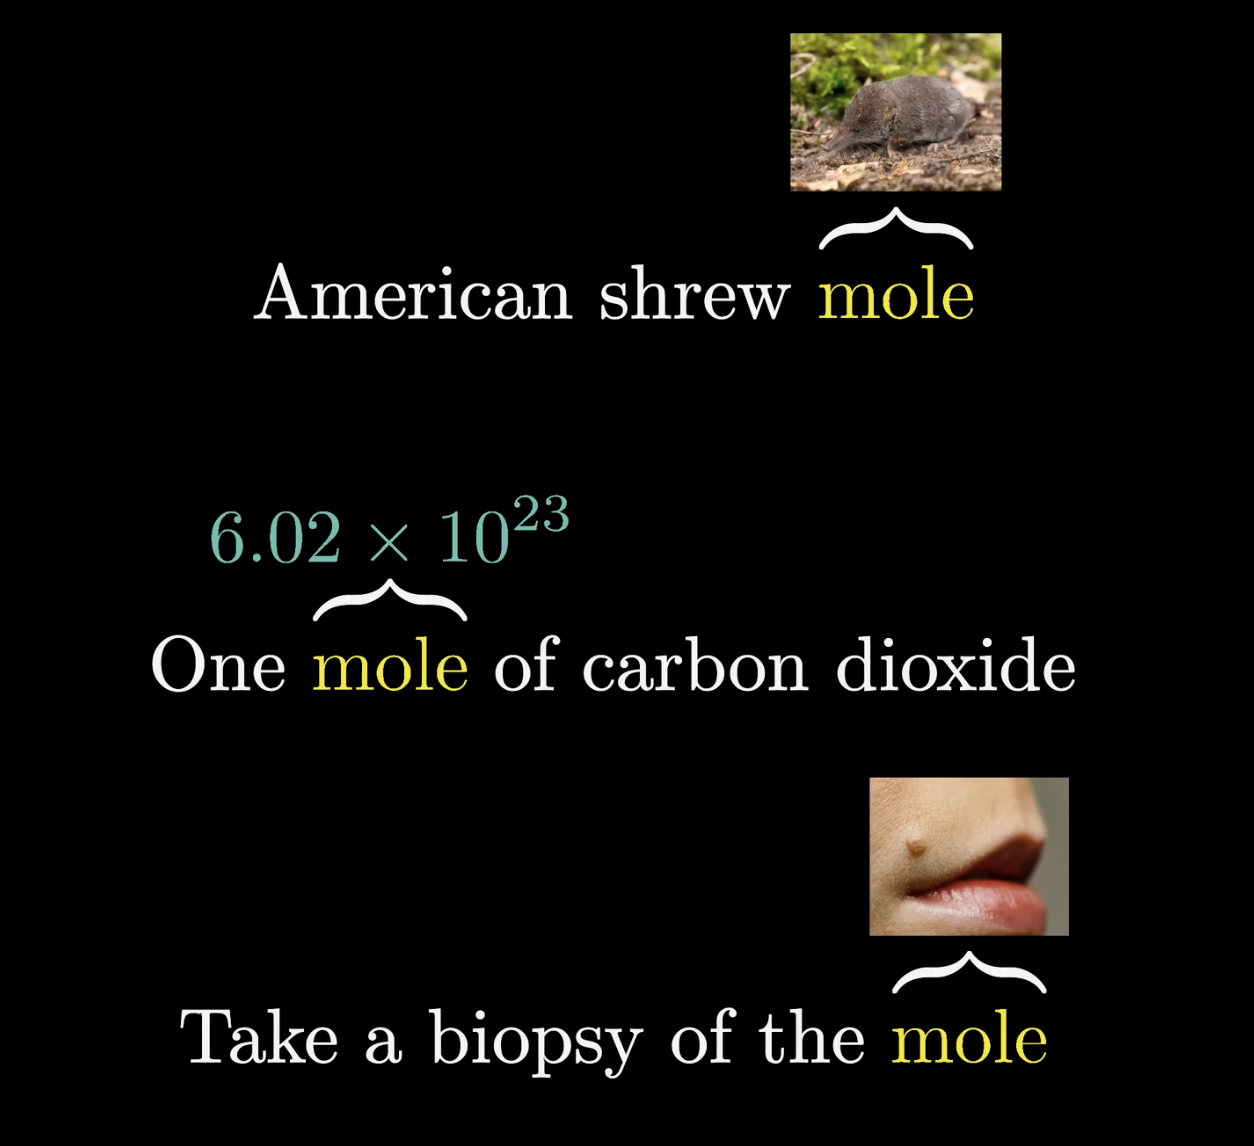
\includegraphics[width=0.7\textwidth]{images/mole} 
\end{figure}
\pause 
\begin{center}
\textbf{Example}:  The word \qq{mole} has various meanings.
\end{center}
\end{frame}


\begin{frame}{Aim of transformer}
\begin{figure} 
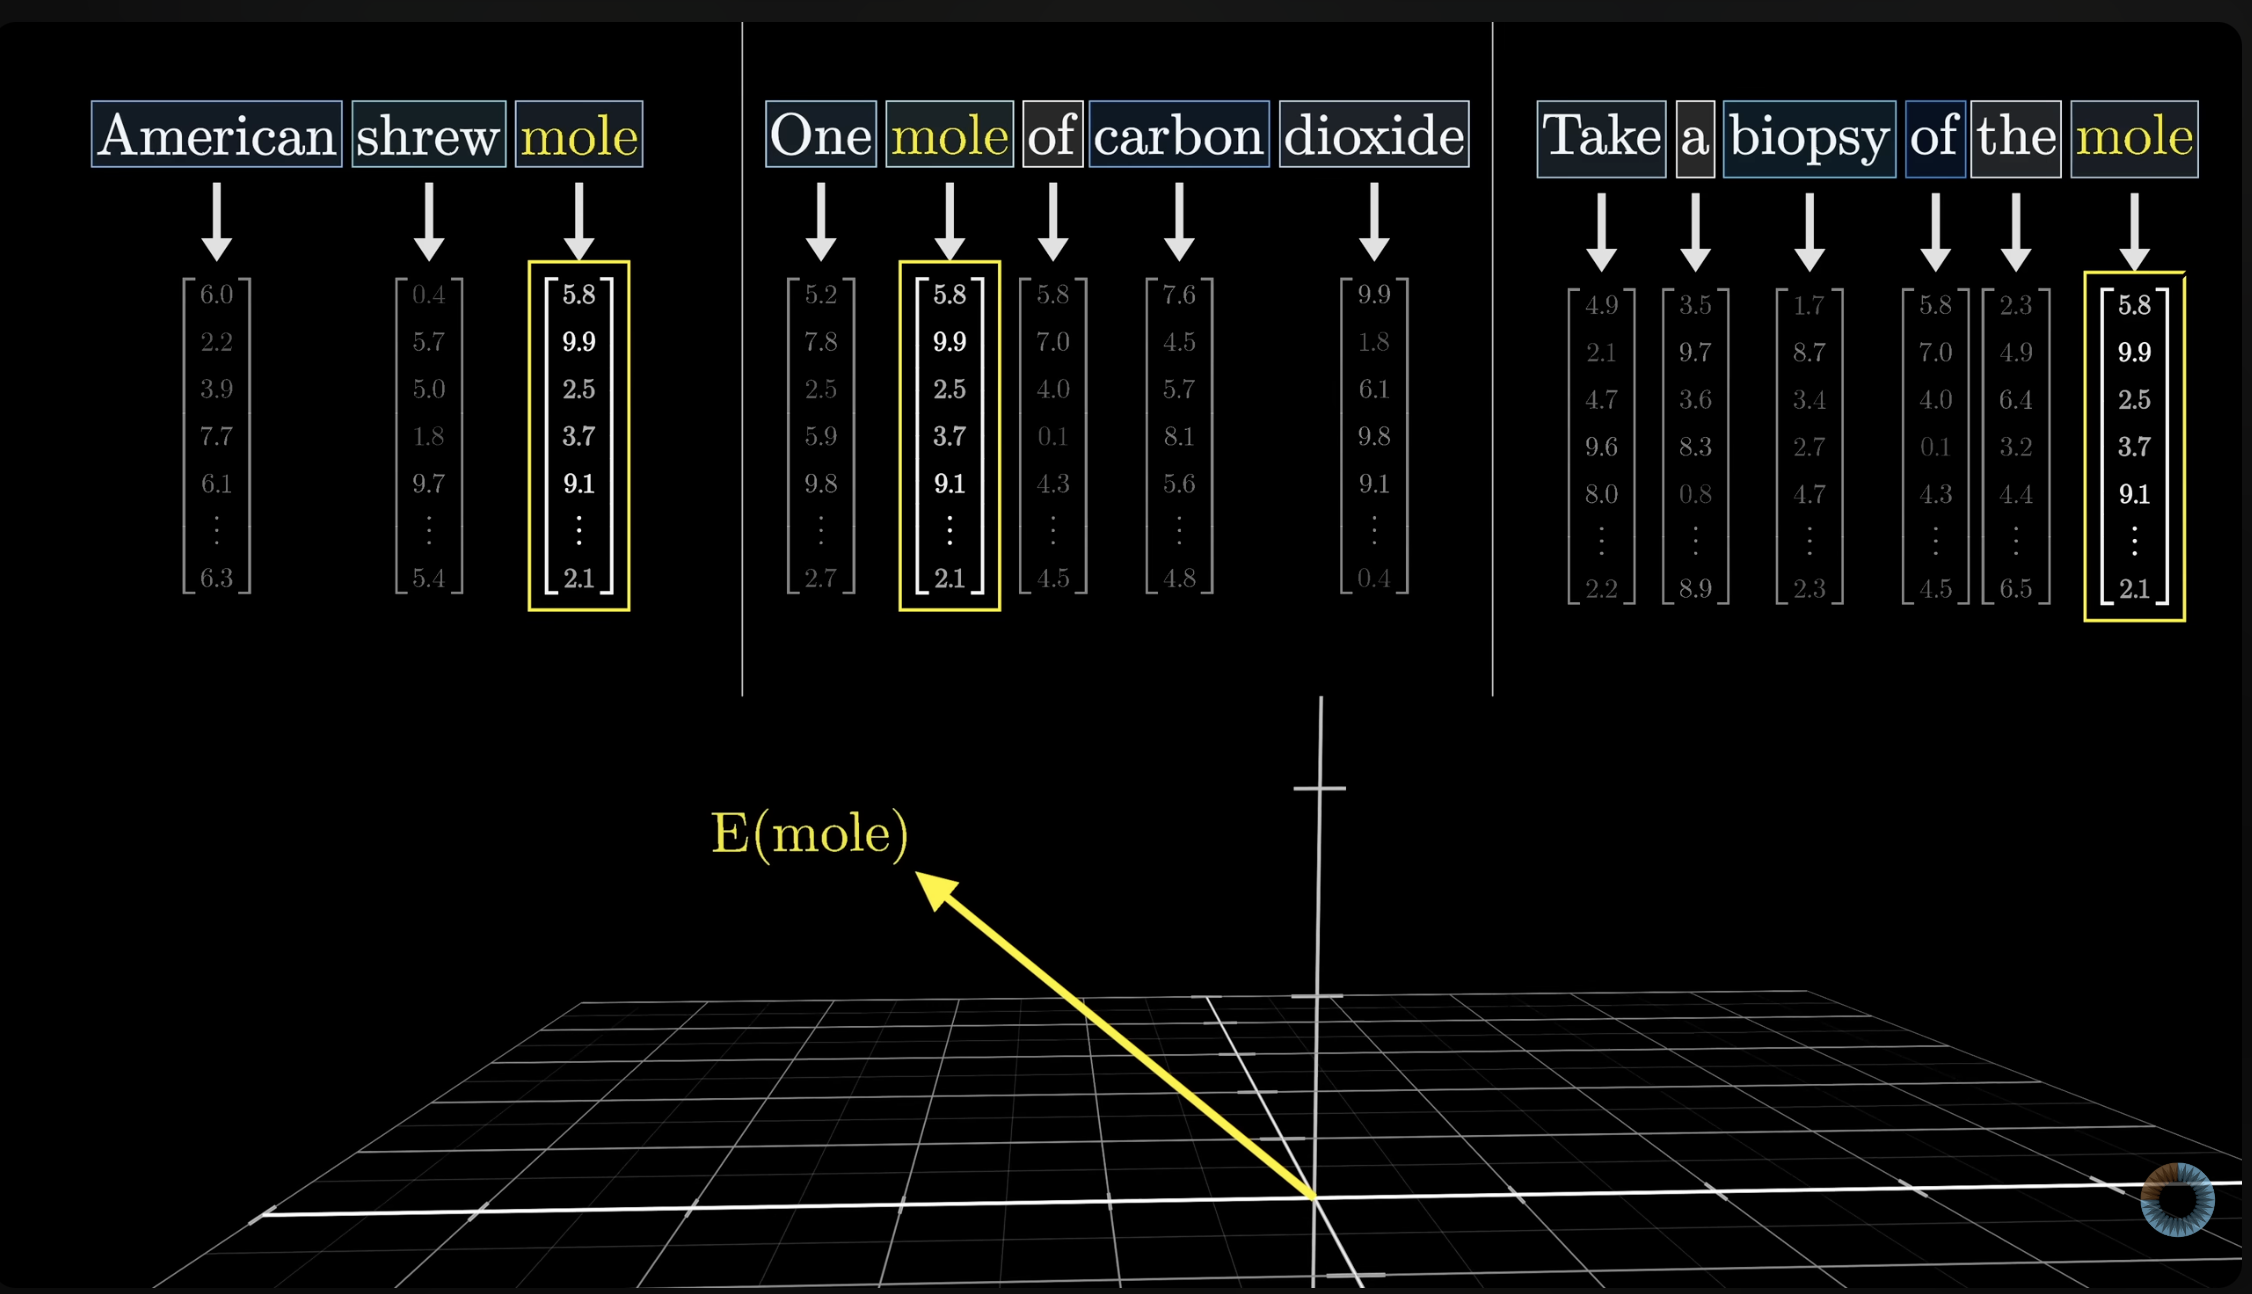
\includegraphics[width=1.0\textwidth]{images/mole2} 
\end{figure}
\pause 
\begin{center}
Initial embedding is the same for all 3 cases.
\pause 
It's a look-up table with no reference to the context.
\end{center}
\end{frame}



\begin{frame}{Aim of transformer}

\begin{center}
\only<1>{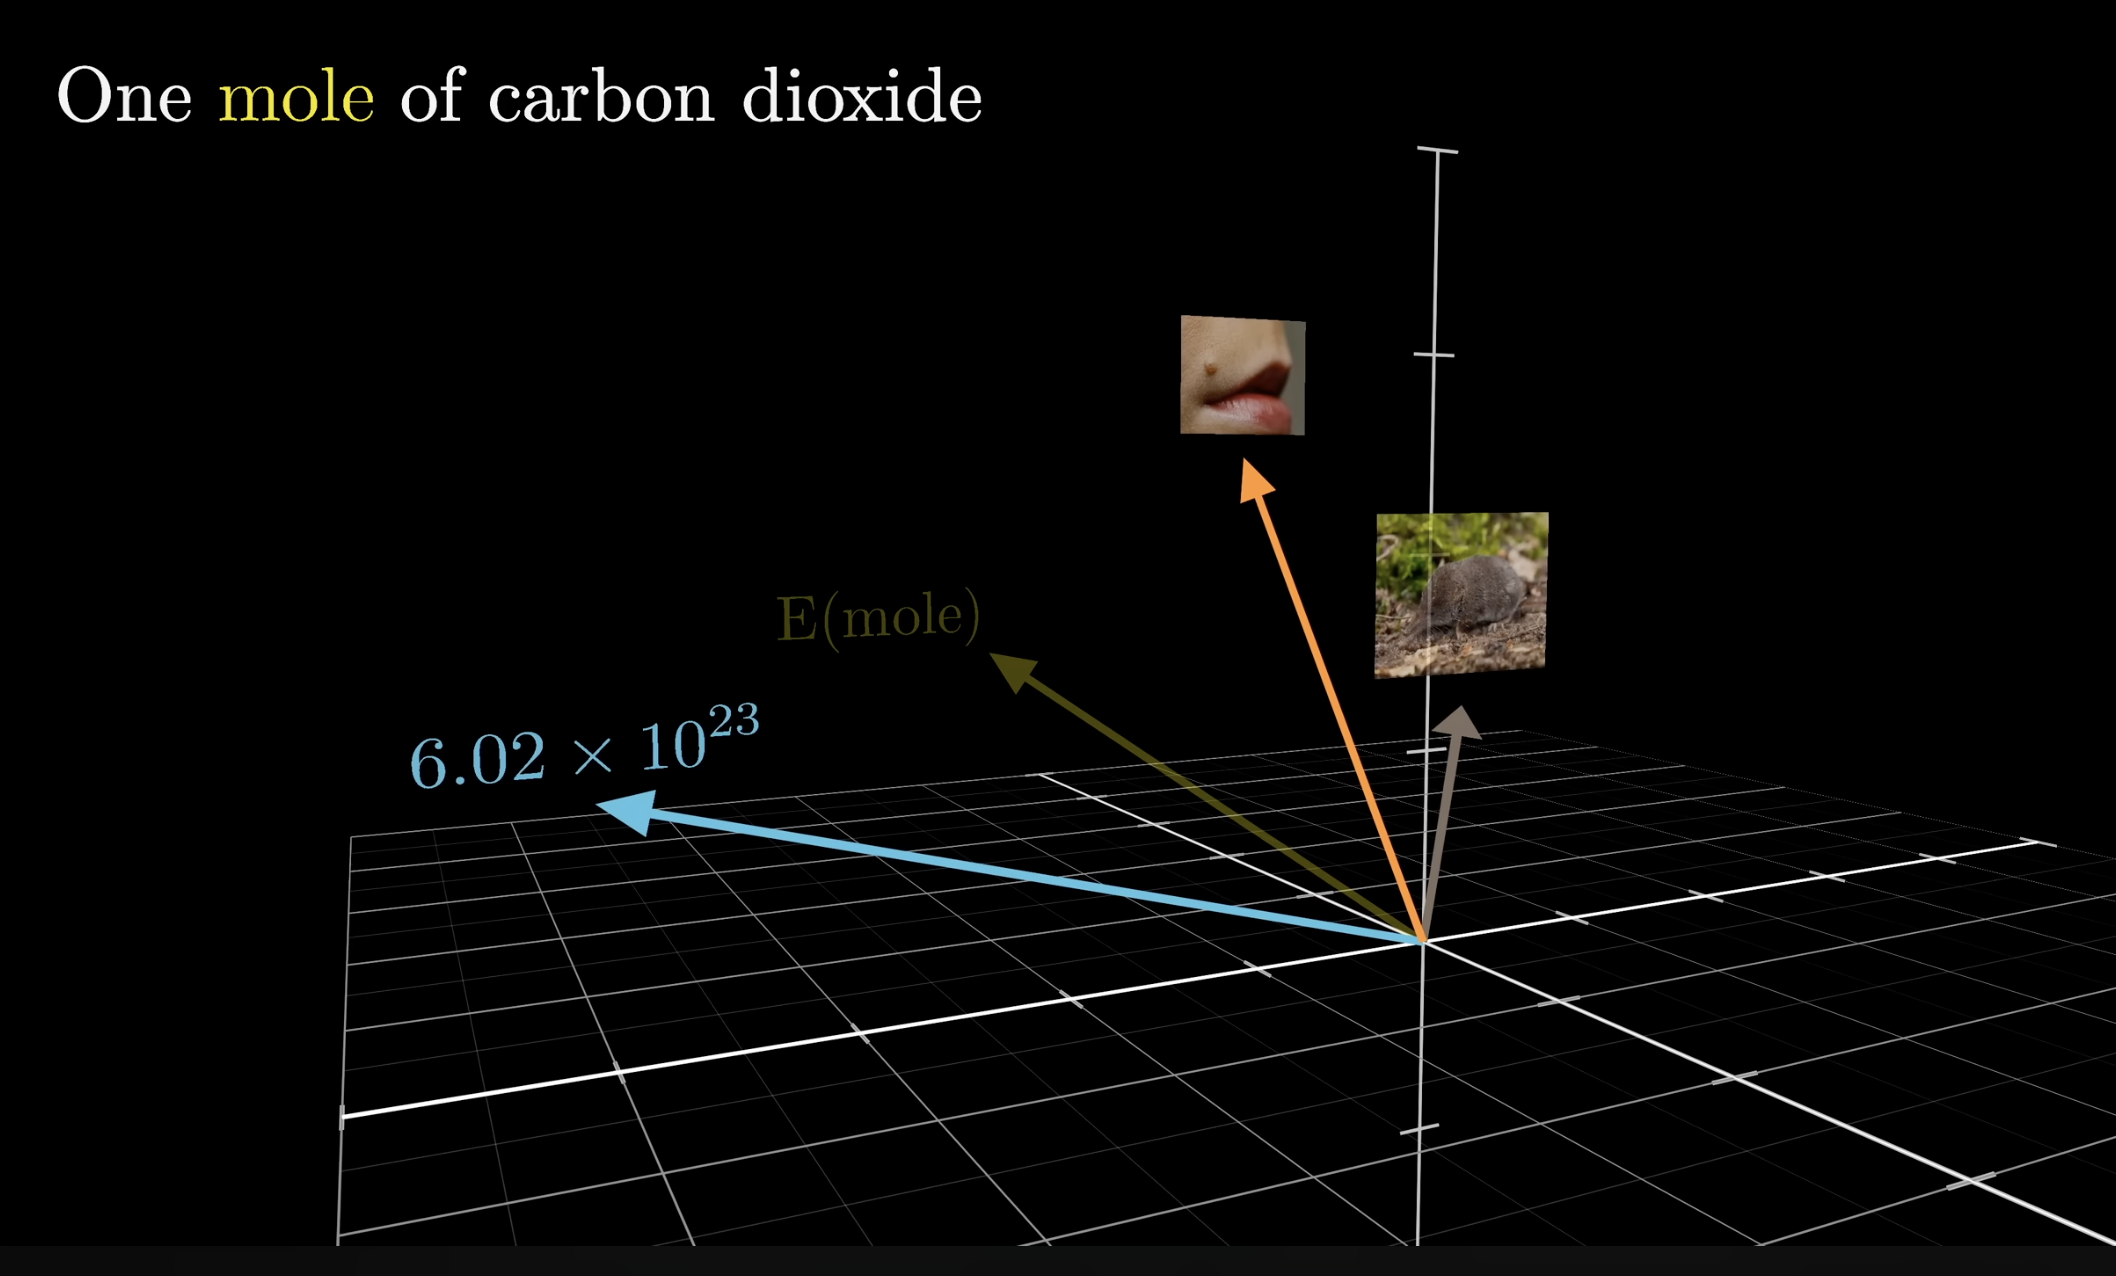
\includegraphics[width=0.85\textwidth]{images/mole_add1}}
\only<2>{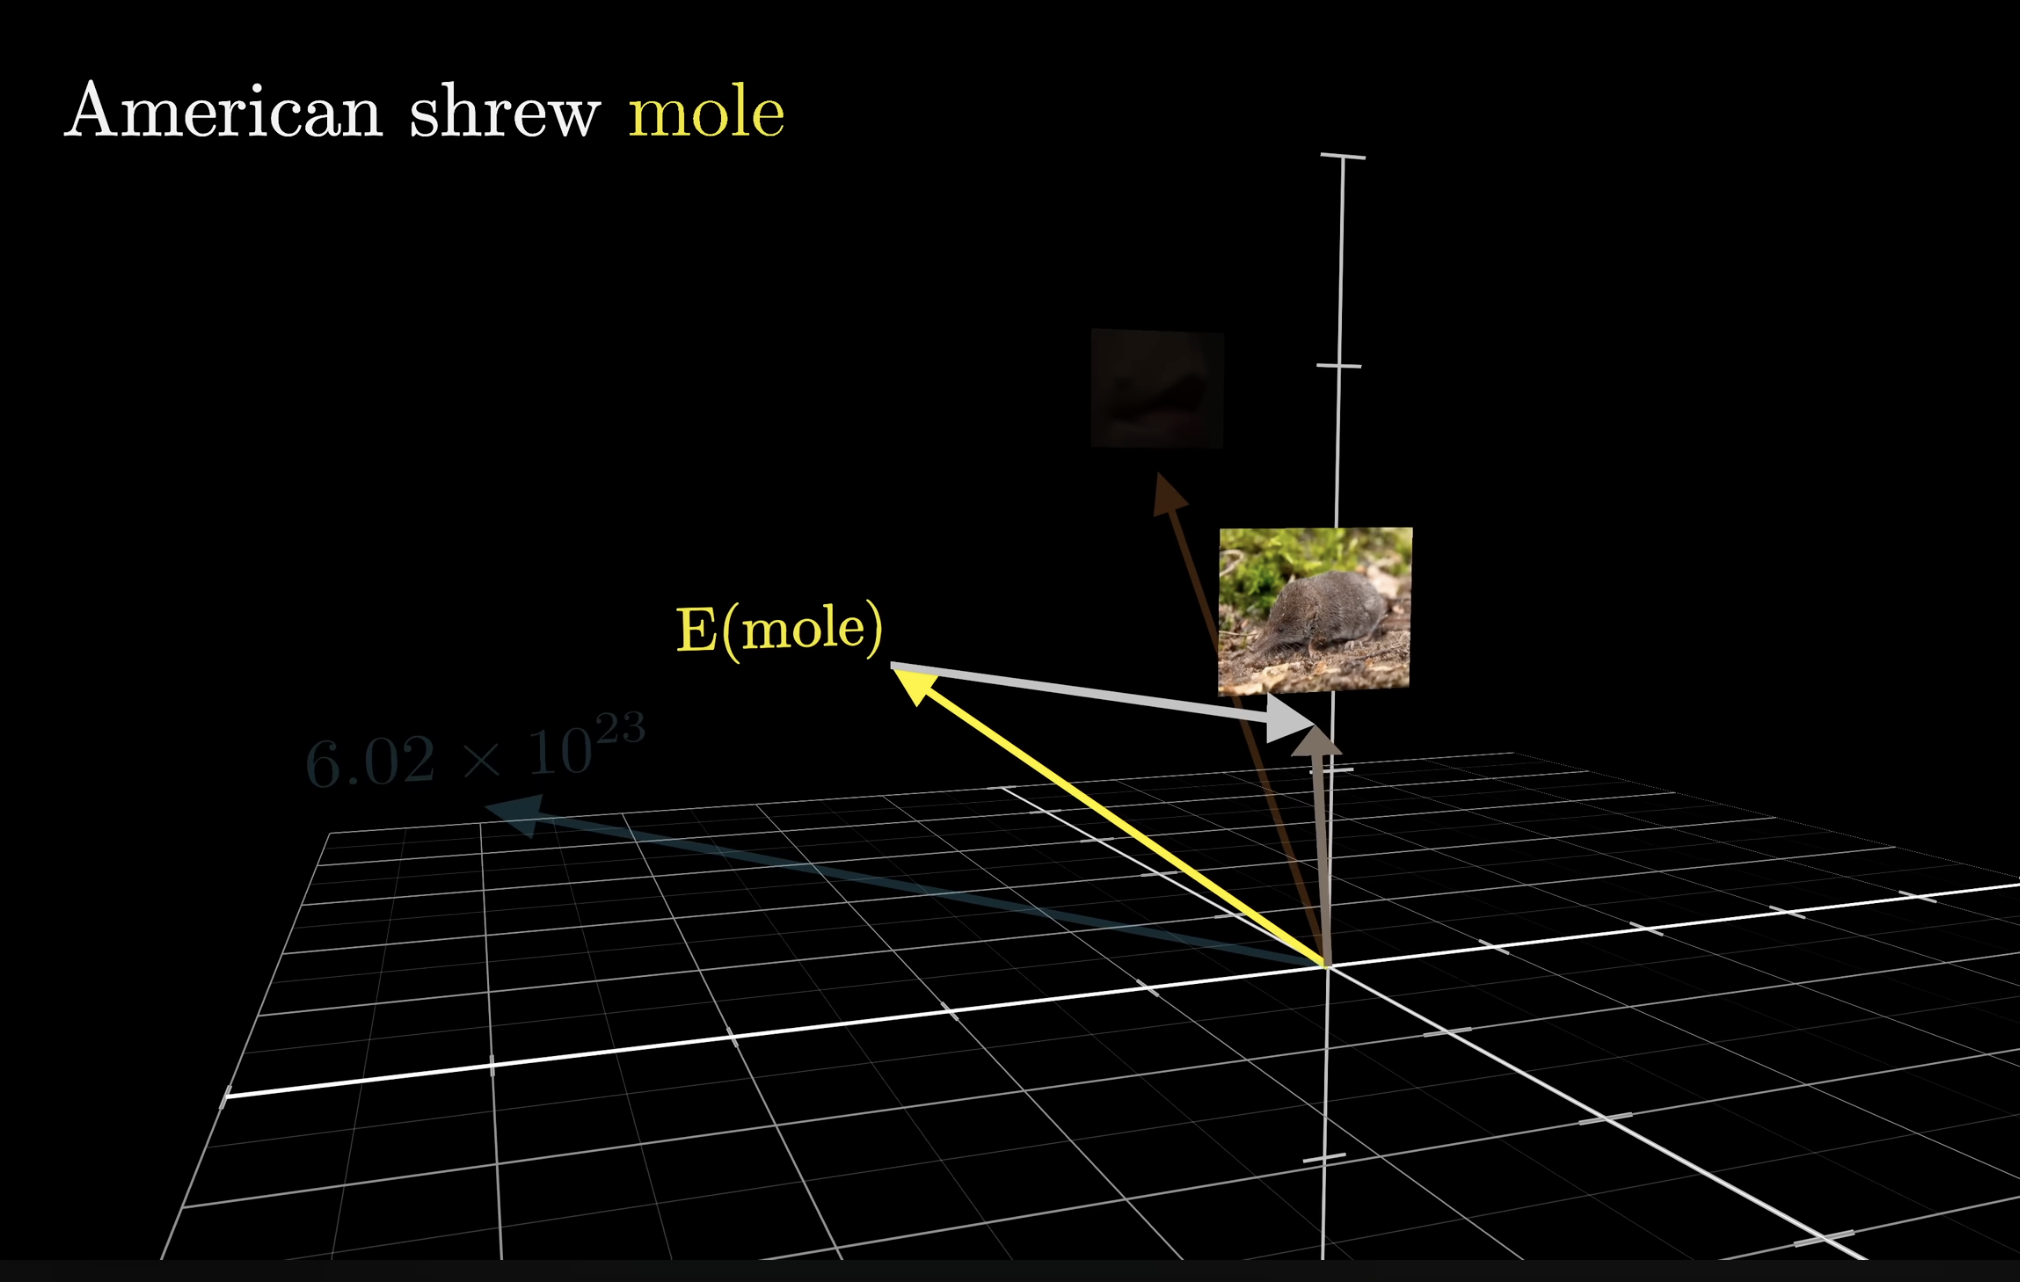
\includegraphics[width=0.85\textwidth]{images/mole_add2}}
\only<3>{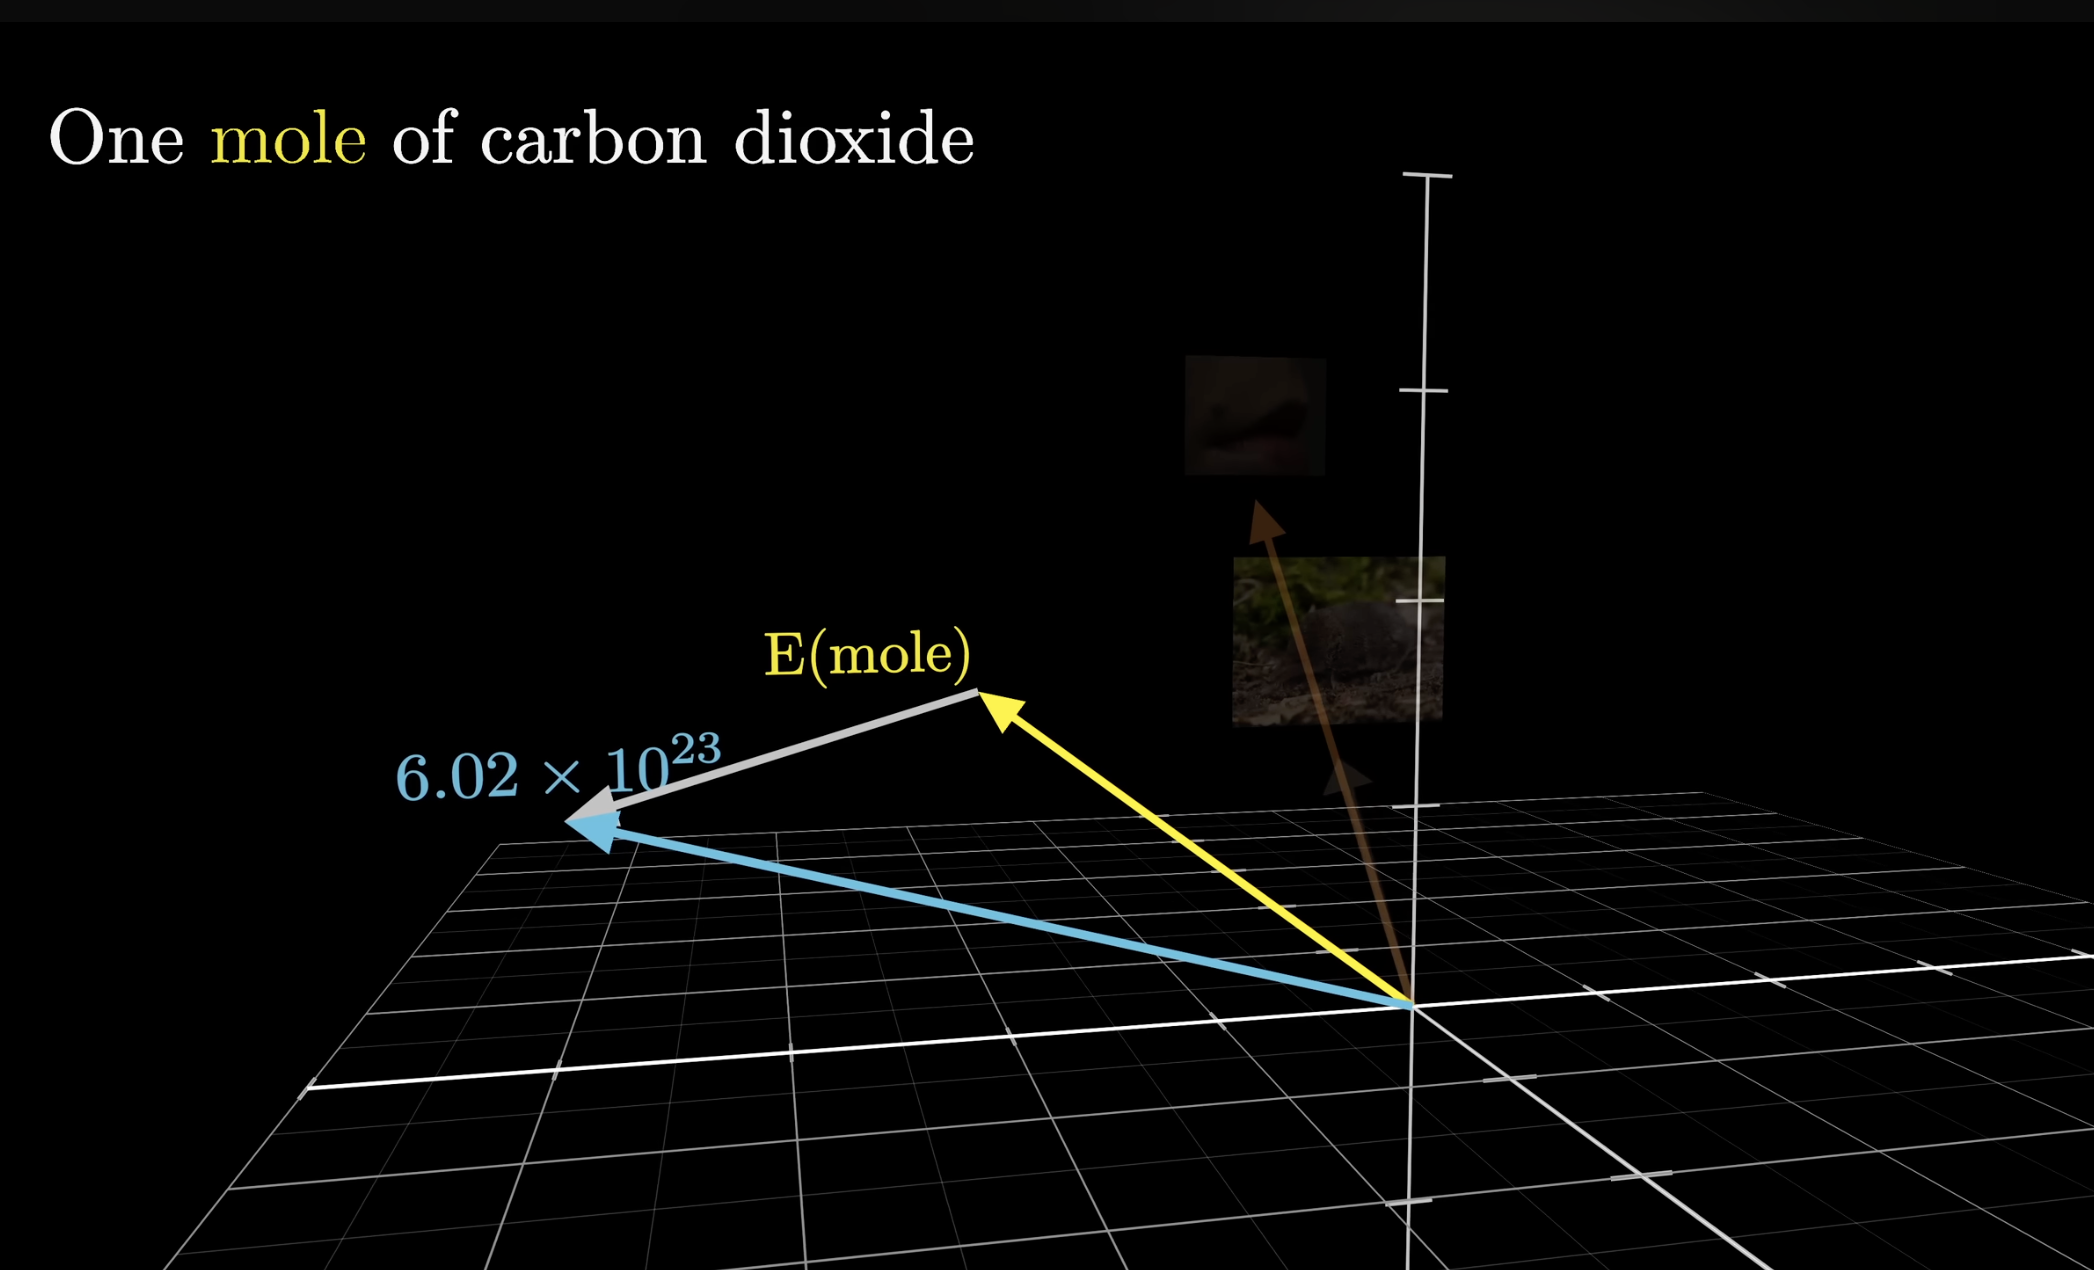
\includegraphics[width=0.85\textwidth]{images/mole_add3}}

\only<1>{
There are multiple directions in embedding space capturing multiple distinct meanings of \qq{mole}.
} 
\only<2-3>{
A well-trained attention block calculates what you need to \alert{add} to the generic embedding to move it to one of these distinct directions.
} 
\end{center}

\end{frame}


\begin{frame}{Aim of transformer}

\begin{center}
\only<1>{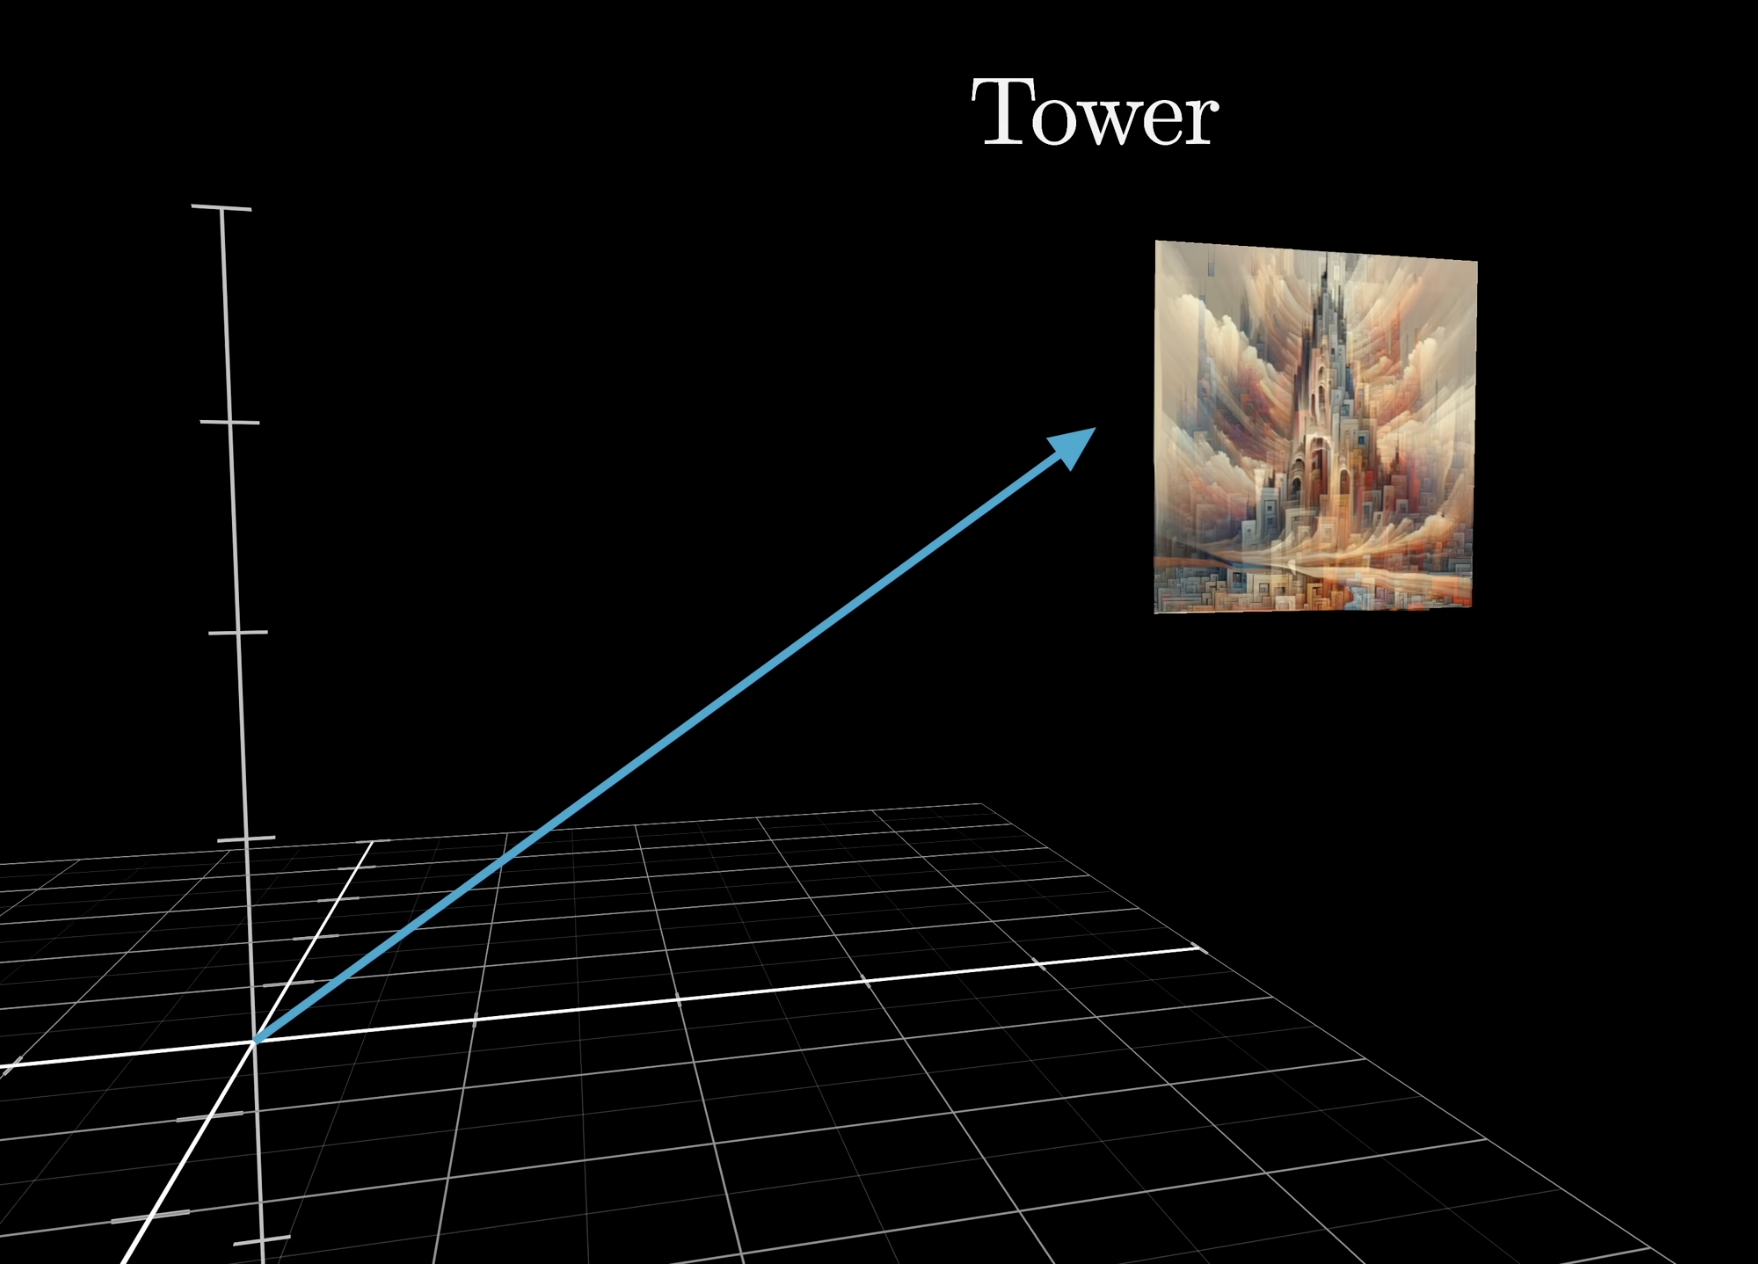
\includegraphics[width=0.85\textwidth]{images/tower1}}
\only<2>{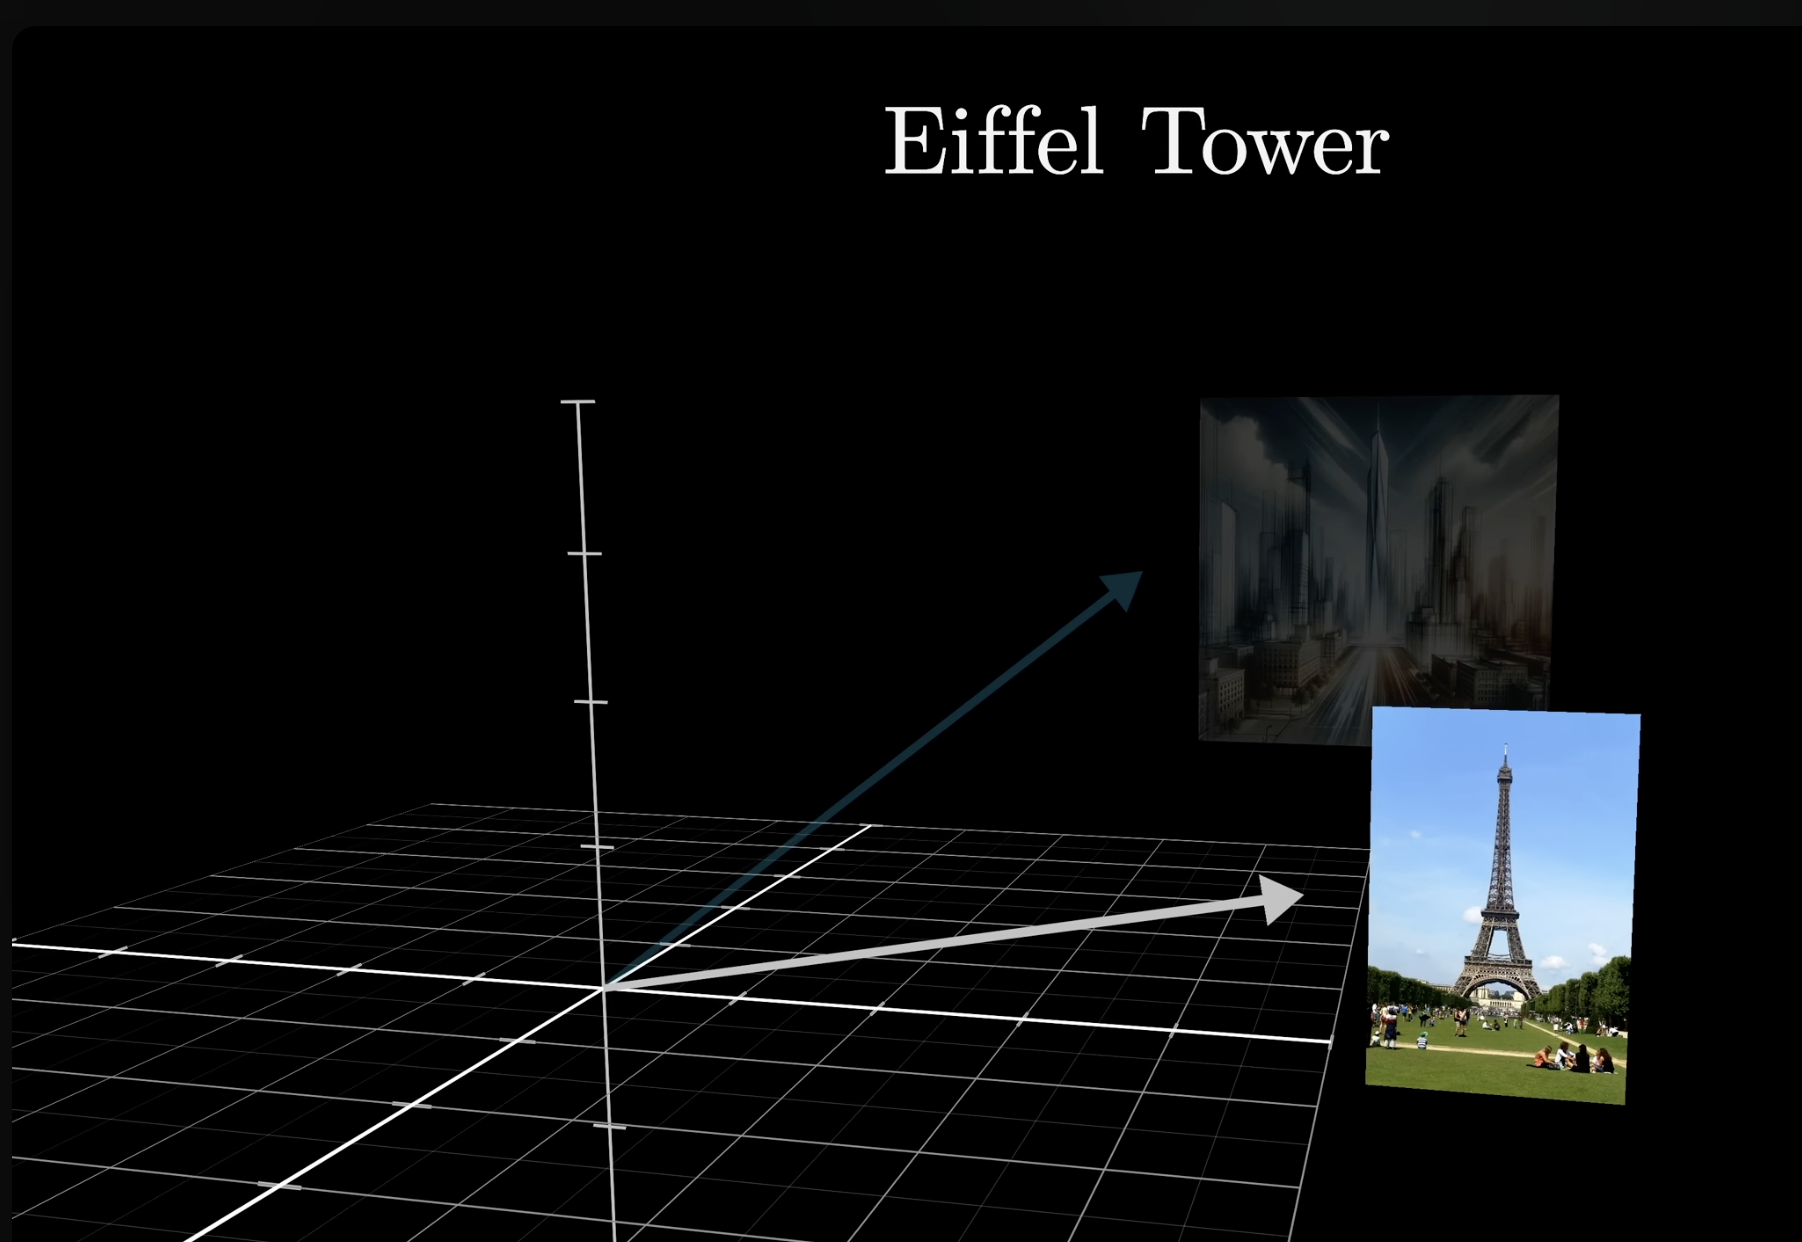
\includegraphics[width=0.85\textwidth]{images/tower2}}
\only<3-4>{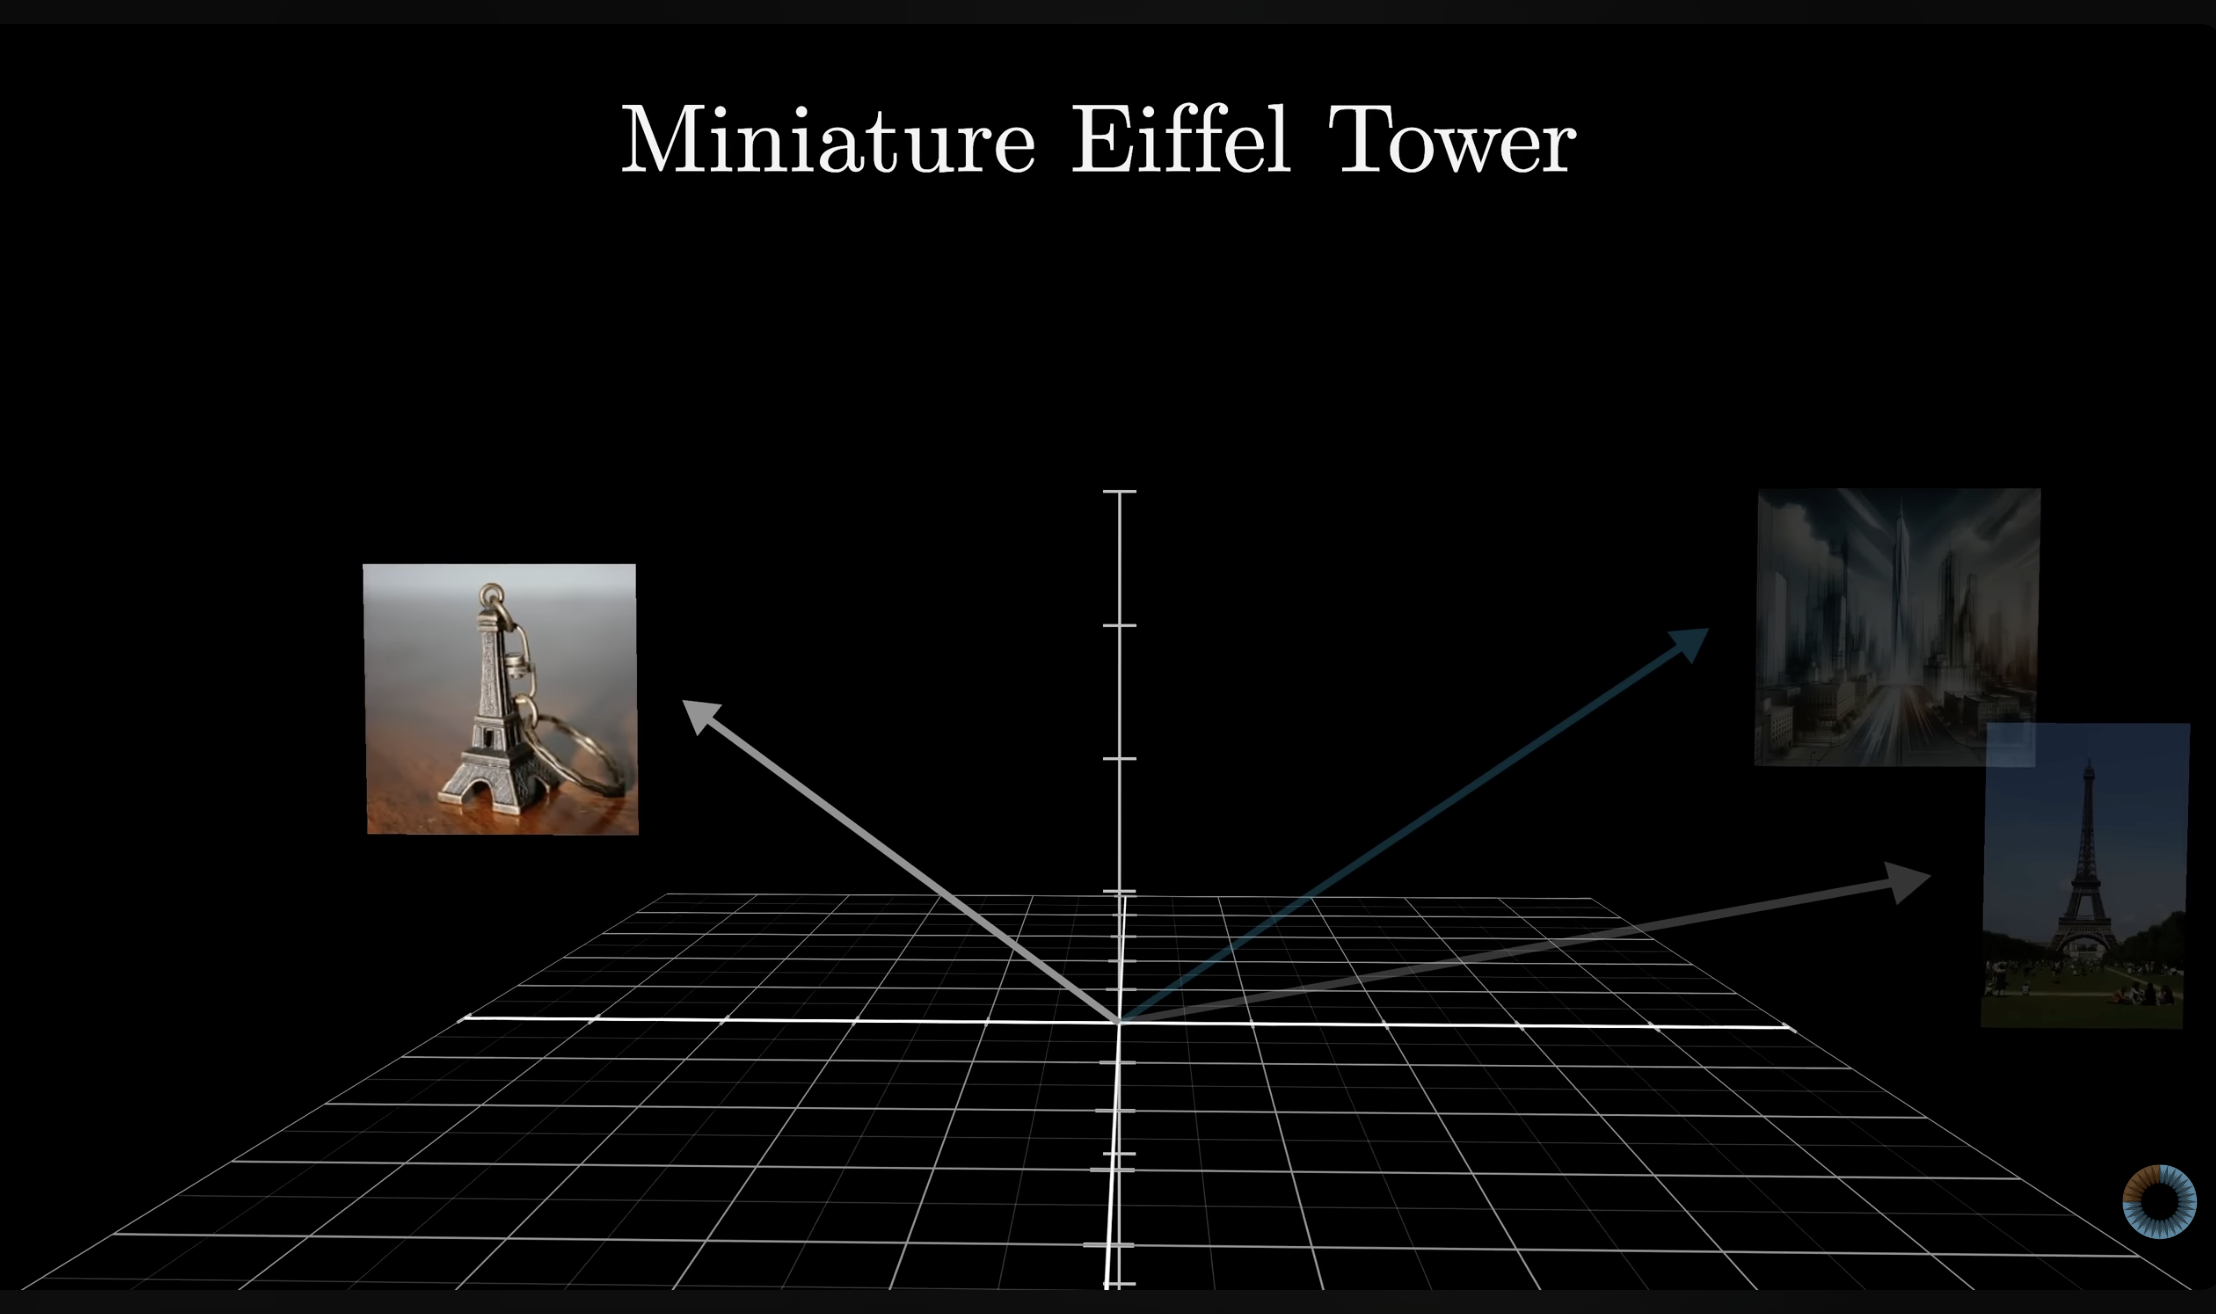
\includegraphics[width=0.85\textwidth]{images/tower3}}

\only<1>{
Starting with the generic embedding for \qq{tower}.
} 
\only<2>{
If preceded by \qq{Eiffel}, we'd want to adjust the embedding towards a direction correlated with Paris, France, steel.
} 
\only<3>{
If \underline{also} preceded by \qq{miniature}, we'd want to adjust the embedding further, so it's no longer correlated with \qq{large tall things}.
} 
\only<4>{
\colorbox{yellow!30}{\textbf{Poll.}} How would you summarize the goal of a transformer?
} 


\end{center}
\end{frame}


\begin{frame}{Aim of transformer}

\begin{center}
\only<1>{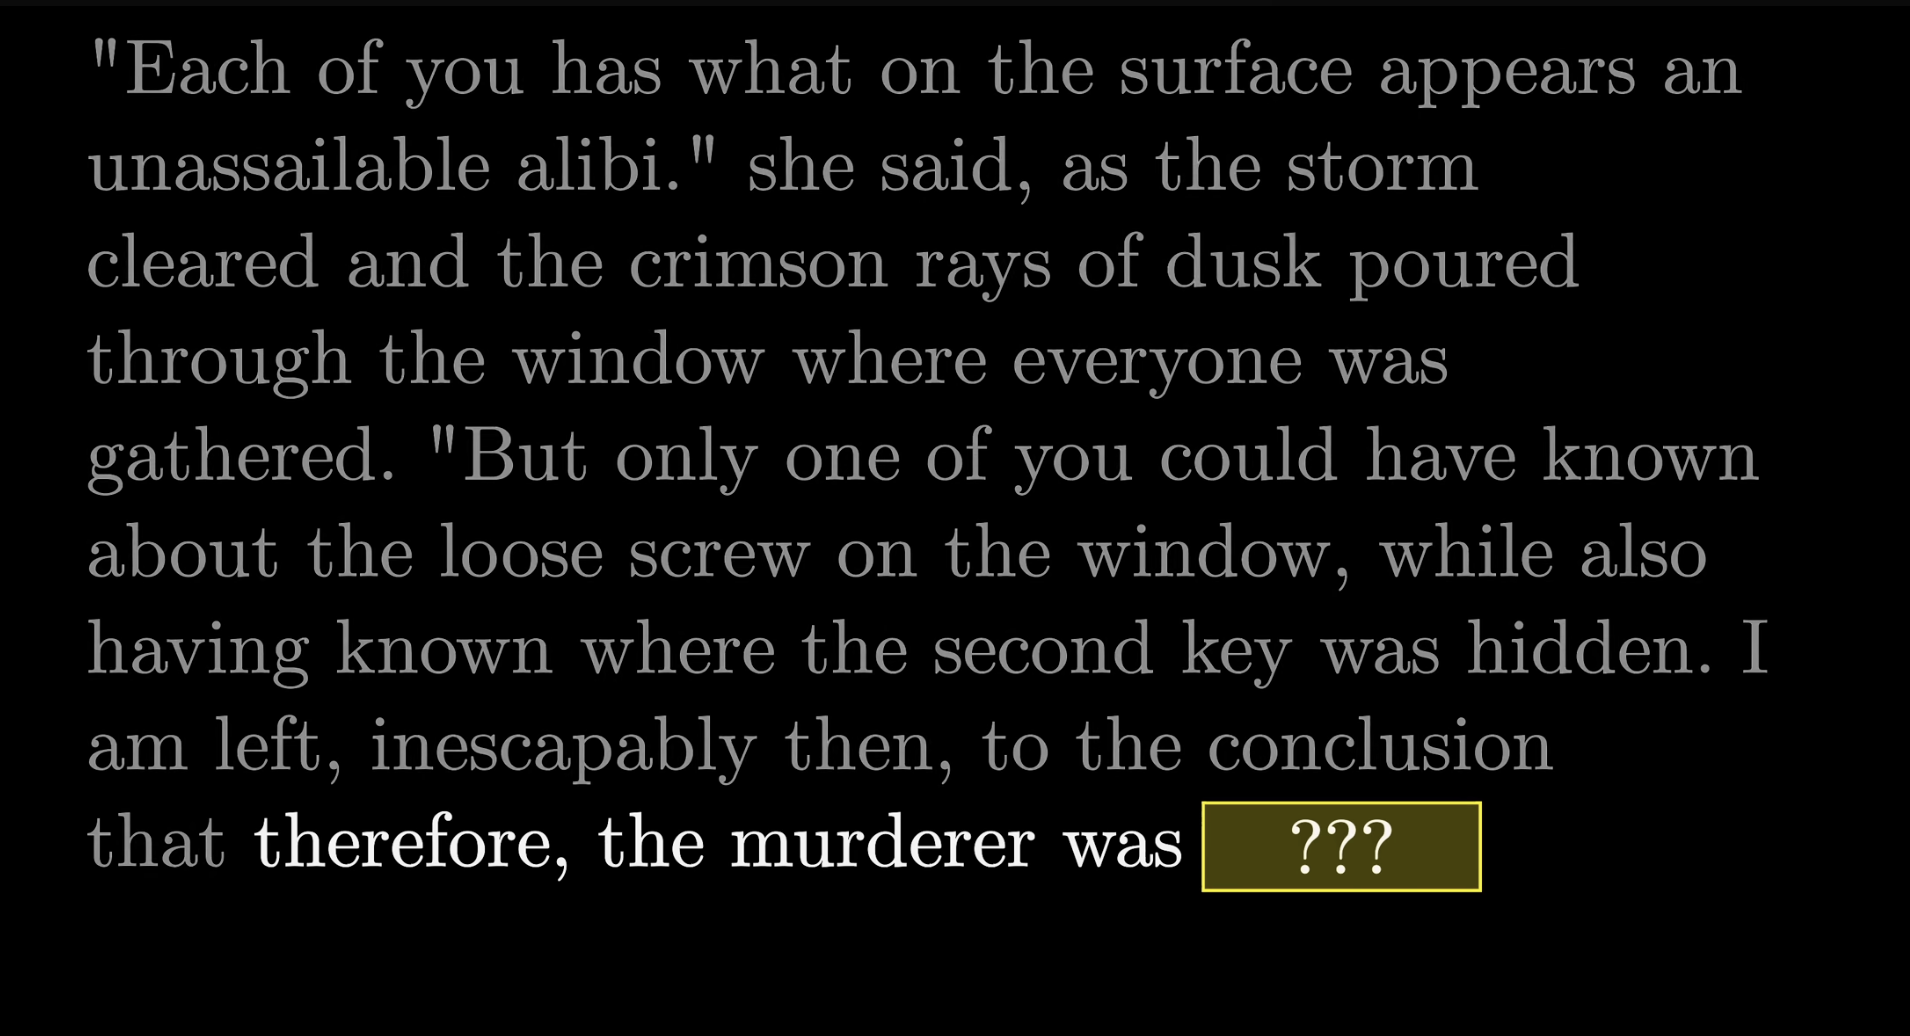
\includegraphics[width=0.85\textwidth]{images/mystery_novel}}

If the context window is large, an entire mystery novel can be encoded in the (updated) embedding for the word \qq{was}!
\end{center}
\end{frame}



\begin{frame}{Single head of attention}

\begin{center}
\only<1->{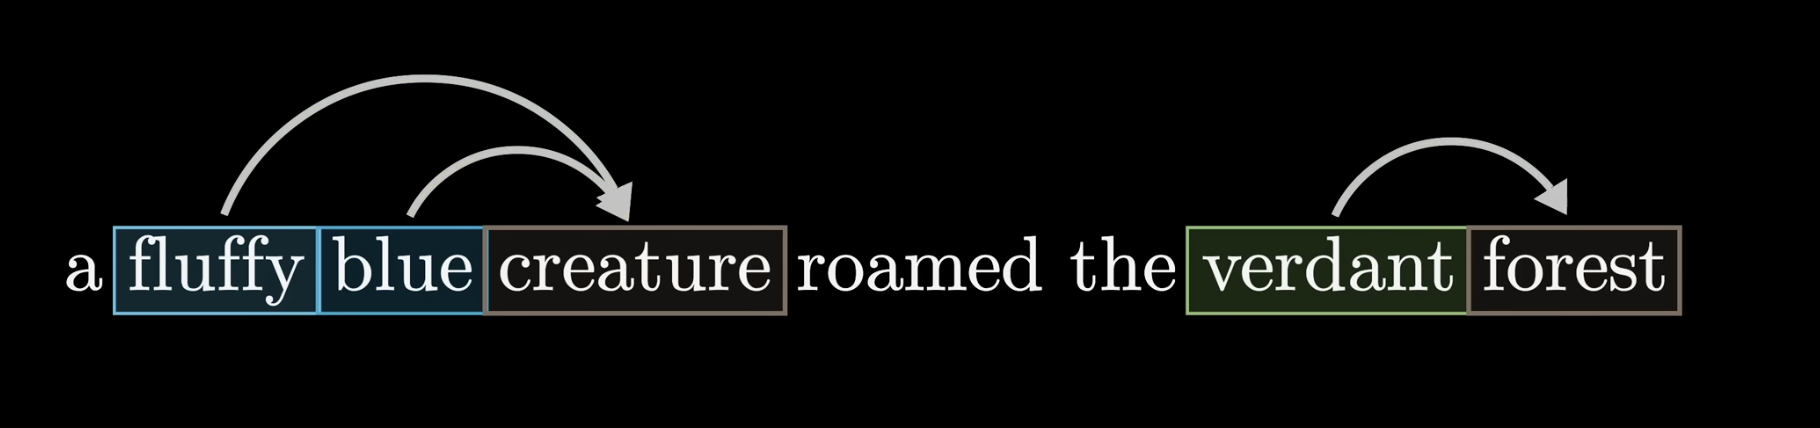
\includegraphics[width=0.85\textwidth]{images/adjectives}}
\end{center}
\vfill  \pause 
\begin{center}
\textbf{Example}: Suppose the only update we care about is to have adjectives adjust the embeddings of their corresponding nouns.
\end{center}
\vfill  \pause 
\begin{center}
\textbf{Remark}:  This processing could be done by a single \alert{head} of attention.  \pause The overall transformer has \underline{multiple} attention heads running in parallel. 
\end{center}
\end{frame}


\begin{frame}{Single head of attention}

\begin{center}
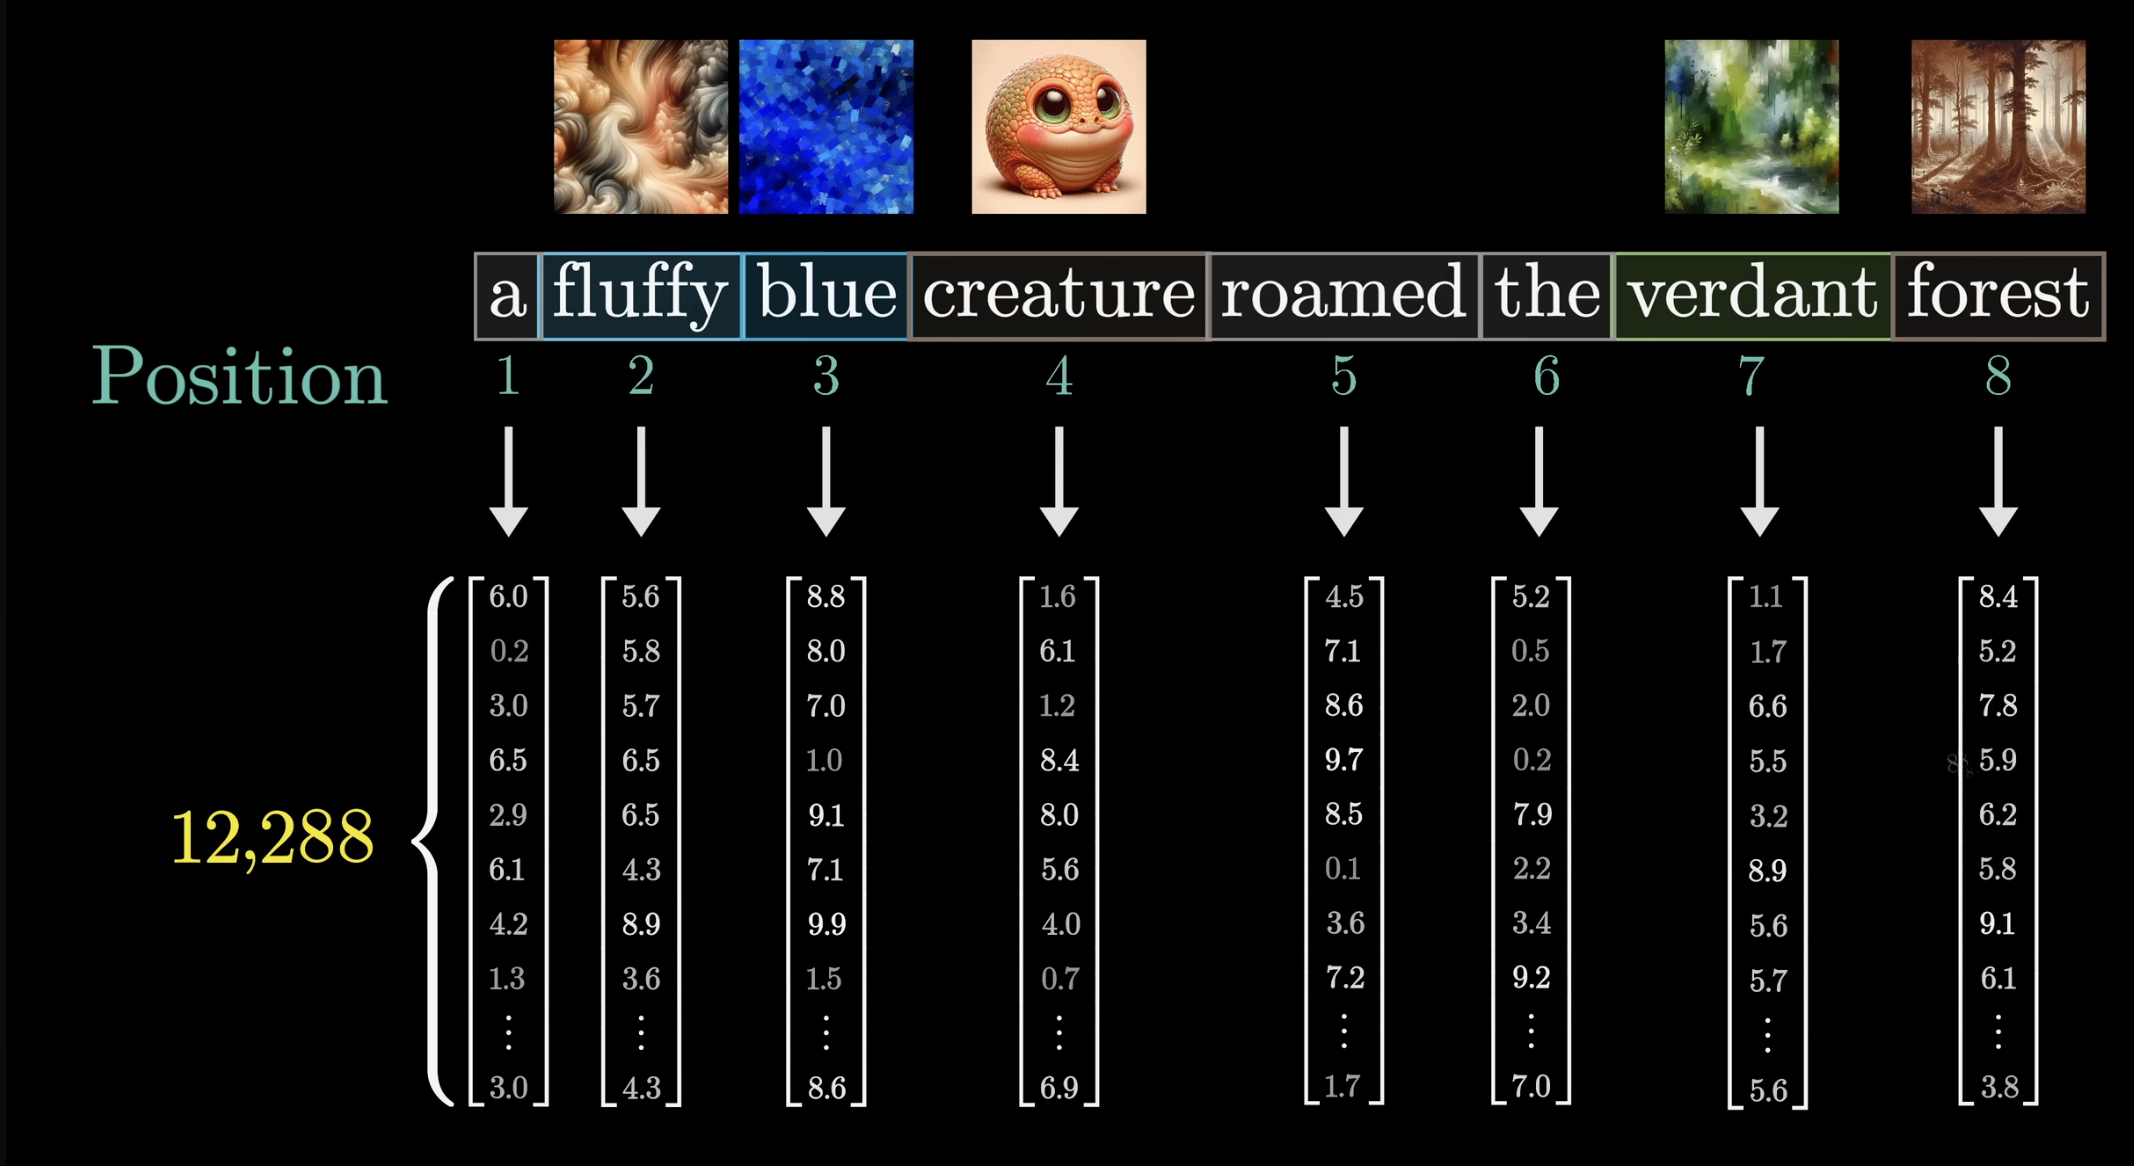
\includegraphics[width=0.85\textwidth]{images/position}
\end{center}
\vfill  \pause 
\begin{center}
The initial embeddings encode two things:

\begin{enumerate}
	\item \textbf{meaning} of individual word with no context
	\item \textbf{position} of the word in the context window
\end{enumerate}
\end{center}
\end{frame}


\begin{frame}{Single head of attention}

\begin{center}
\only<1->{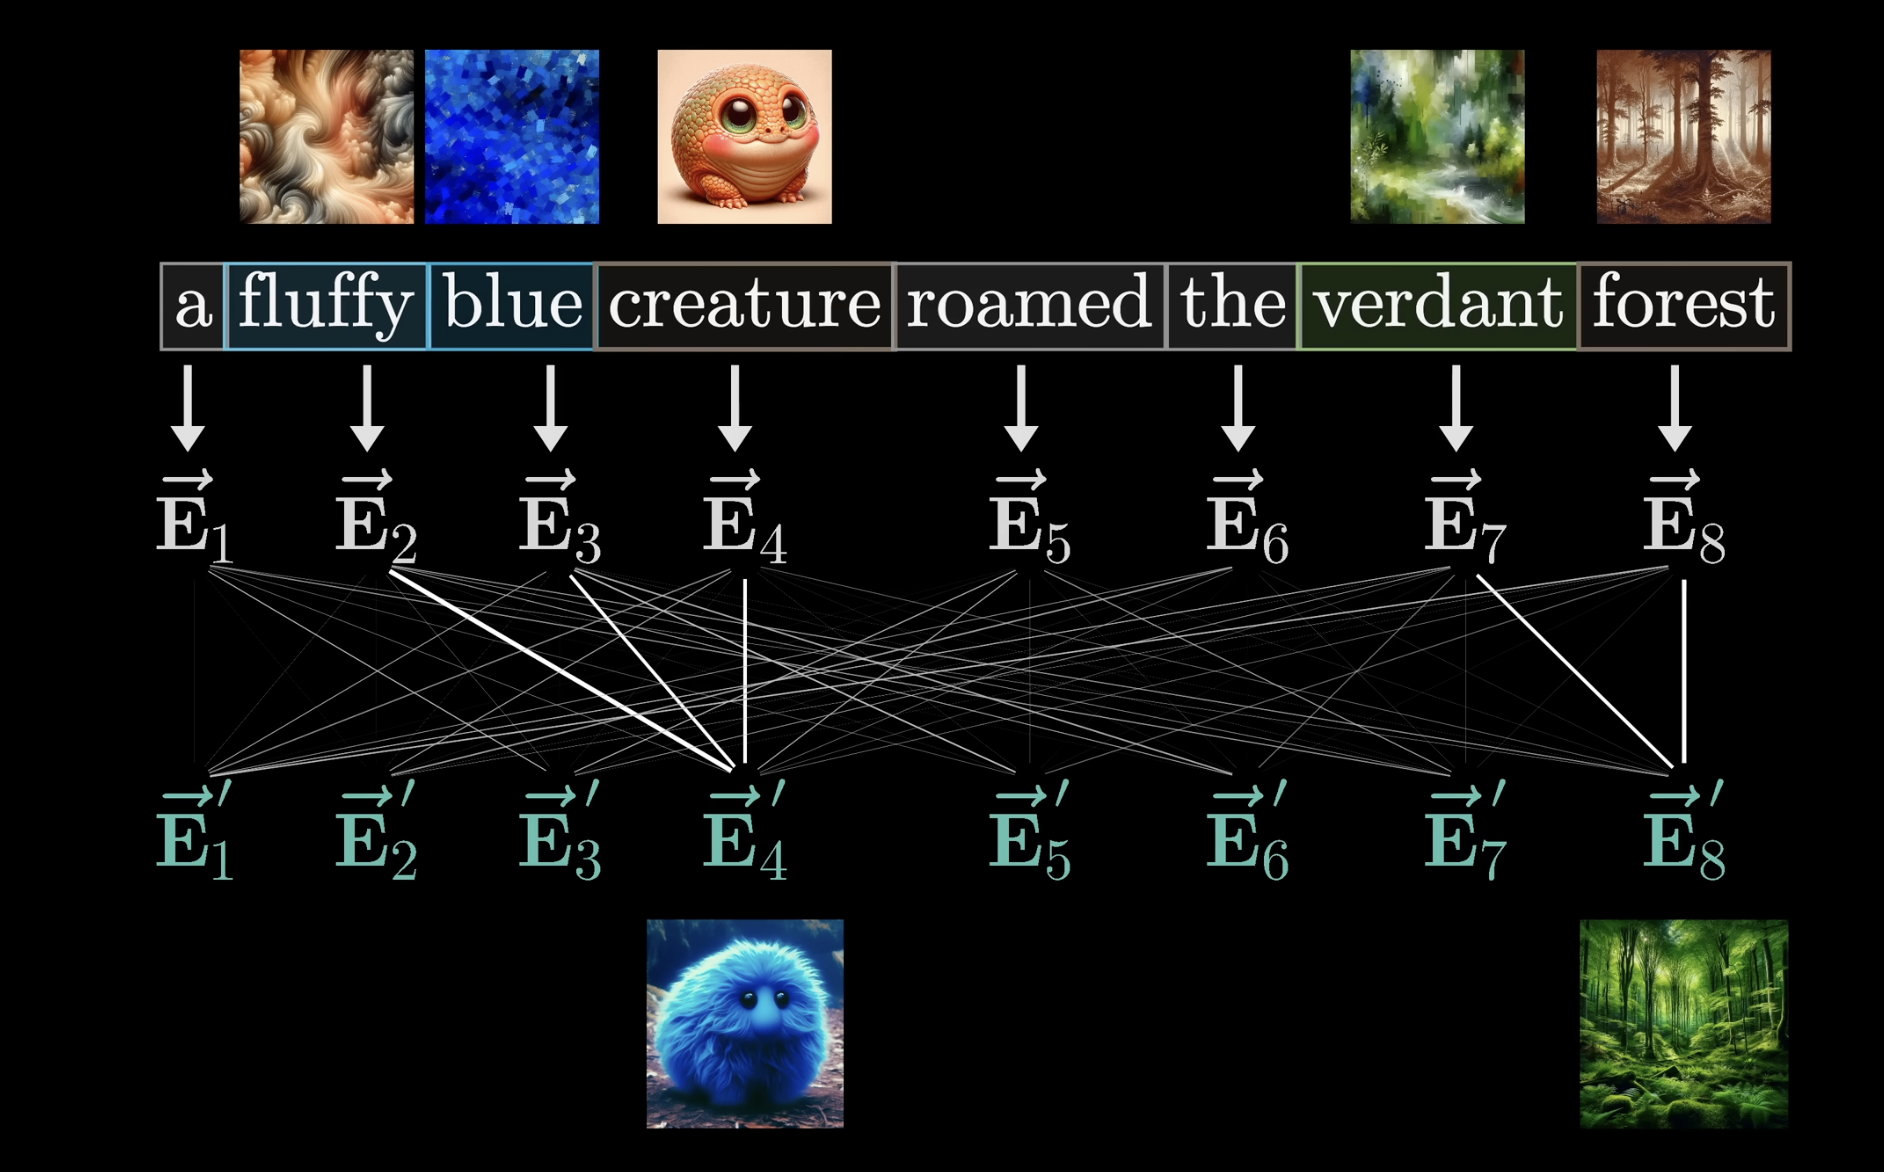
\includegraphics[width=0.85\textwidth]{images/ingest}}
\end{center}
\vfill  \pause 
\begin{center}
\textbf{Goal:} Adjust embeddings so nouns \qq{ingest} the meaning of their corresponding adjectives.
\end{center}
\end{frame}


\begin{frame}{Single head of attention}

\begin{center}

\only<1>{
Imagine each noun asking the question
} 
\only<2>{
And the adjectives before it answering
} 

\only<1>{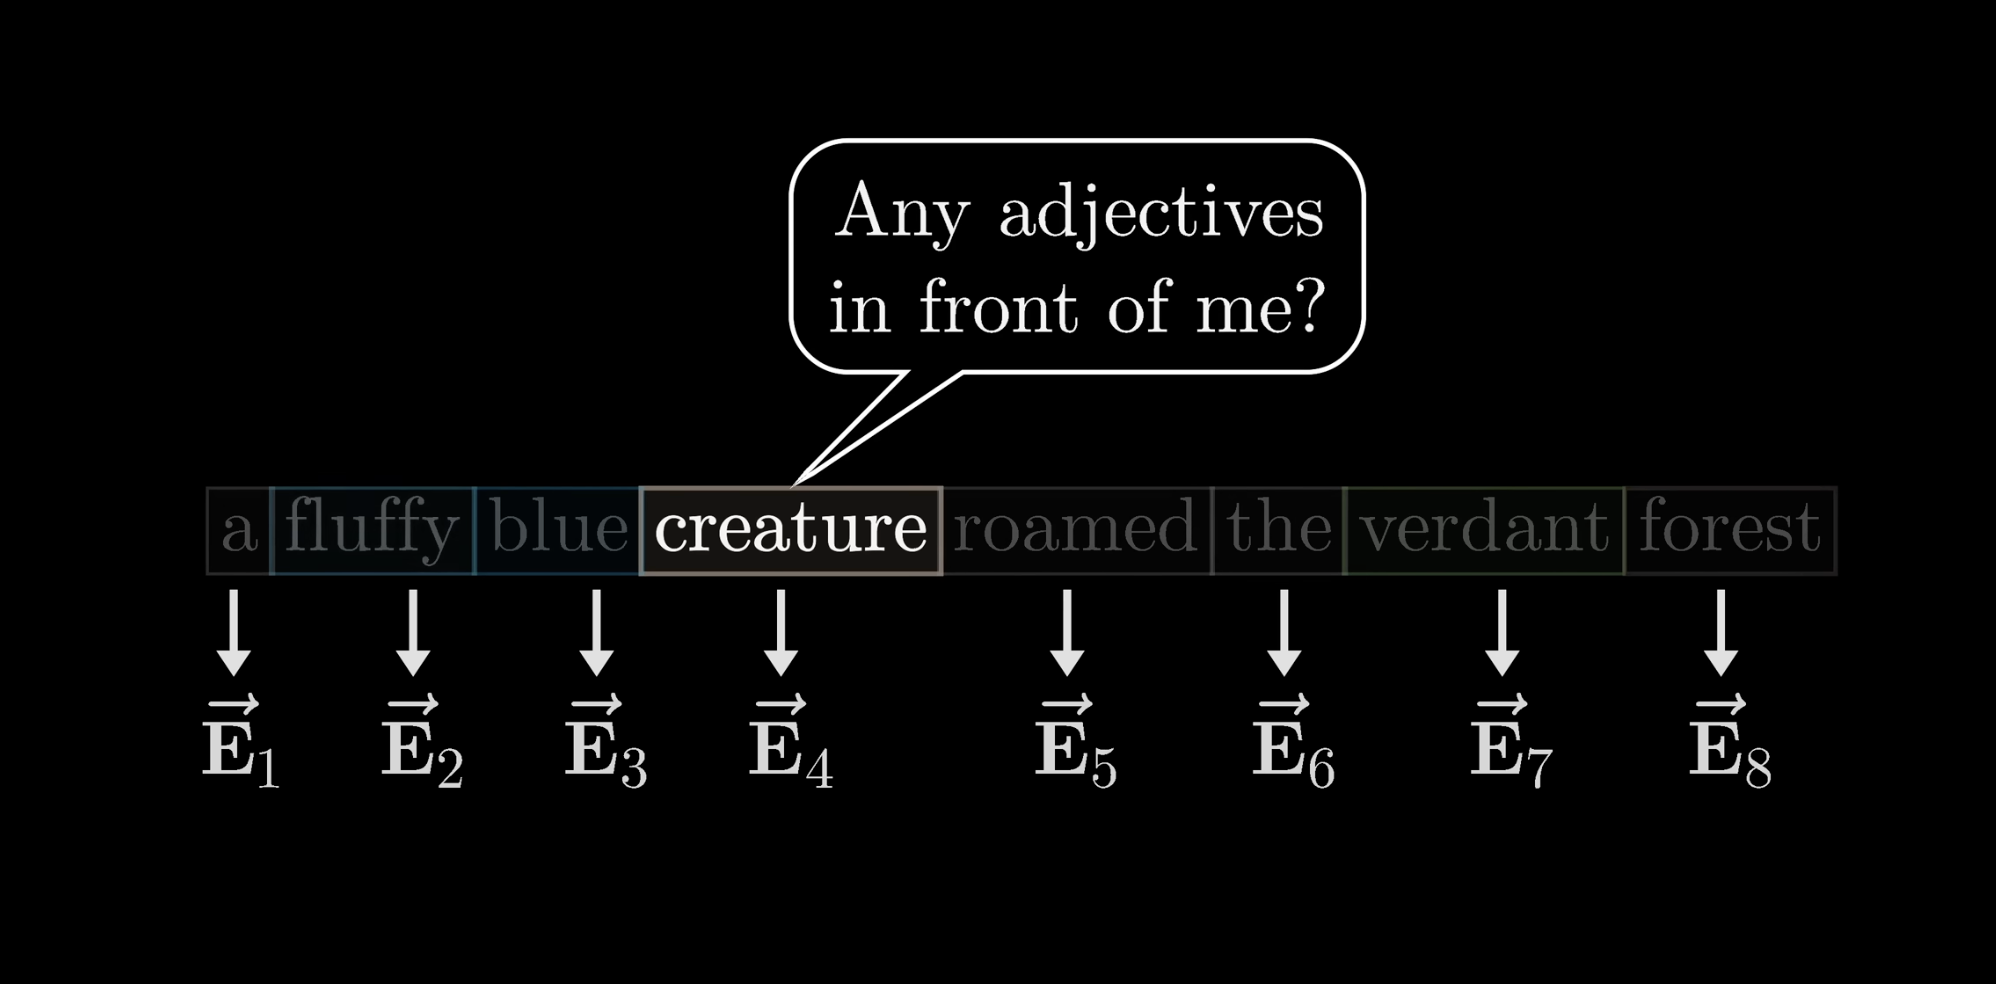
\includegraphics[width=0.85\textwidth]{images/qa1}}
\only<2>{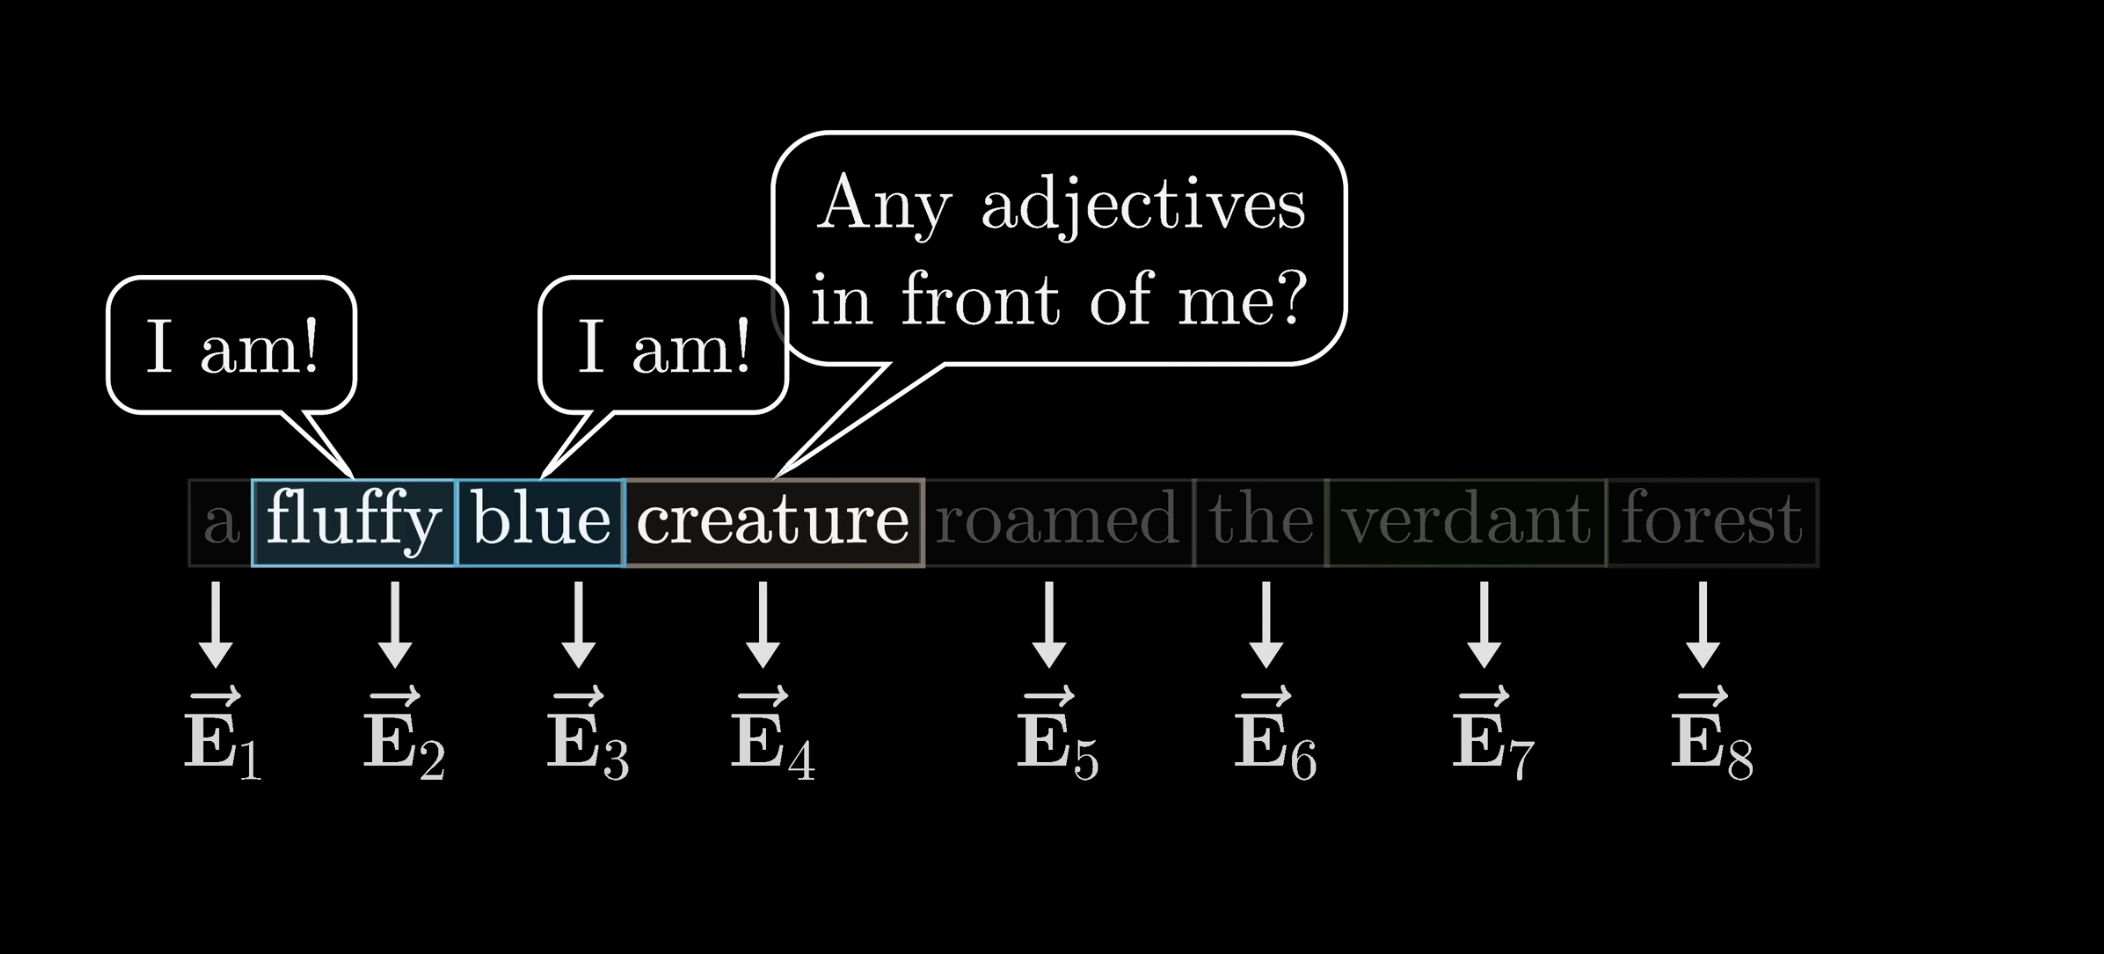
\includegraphics[width=0.85\textwidth]{images/qa2}}



\end{center}

\end{frame}


\begin{frame}{Single head of attention}

\begin{center}


\only<1->{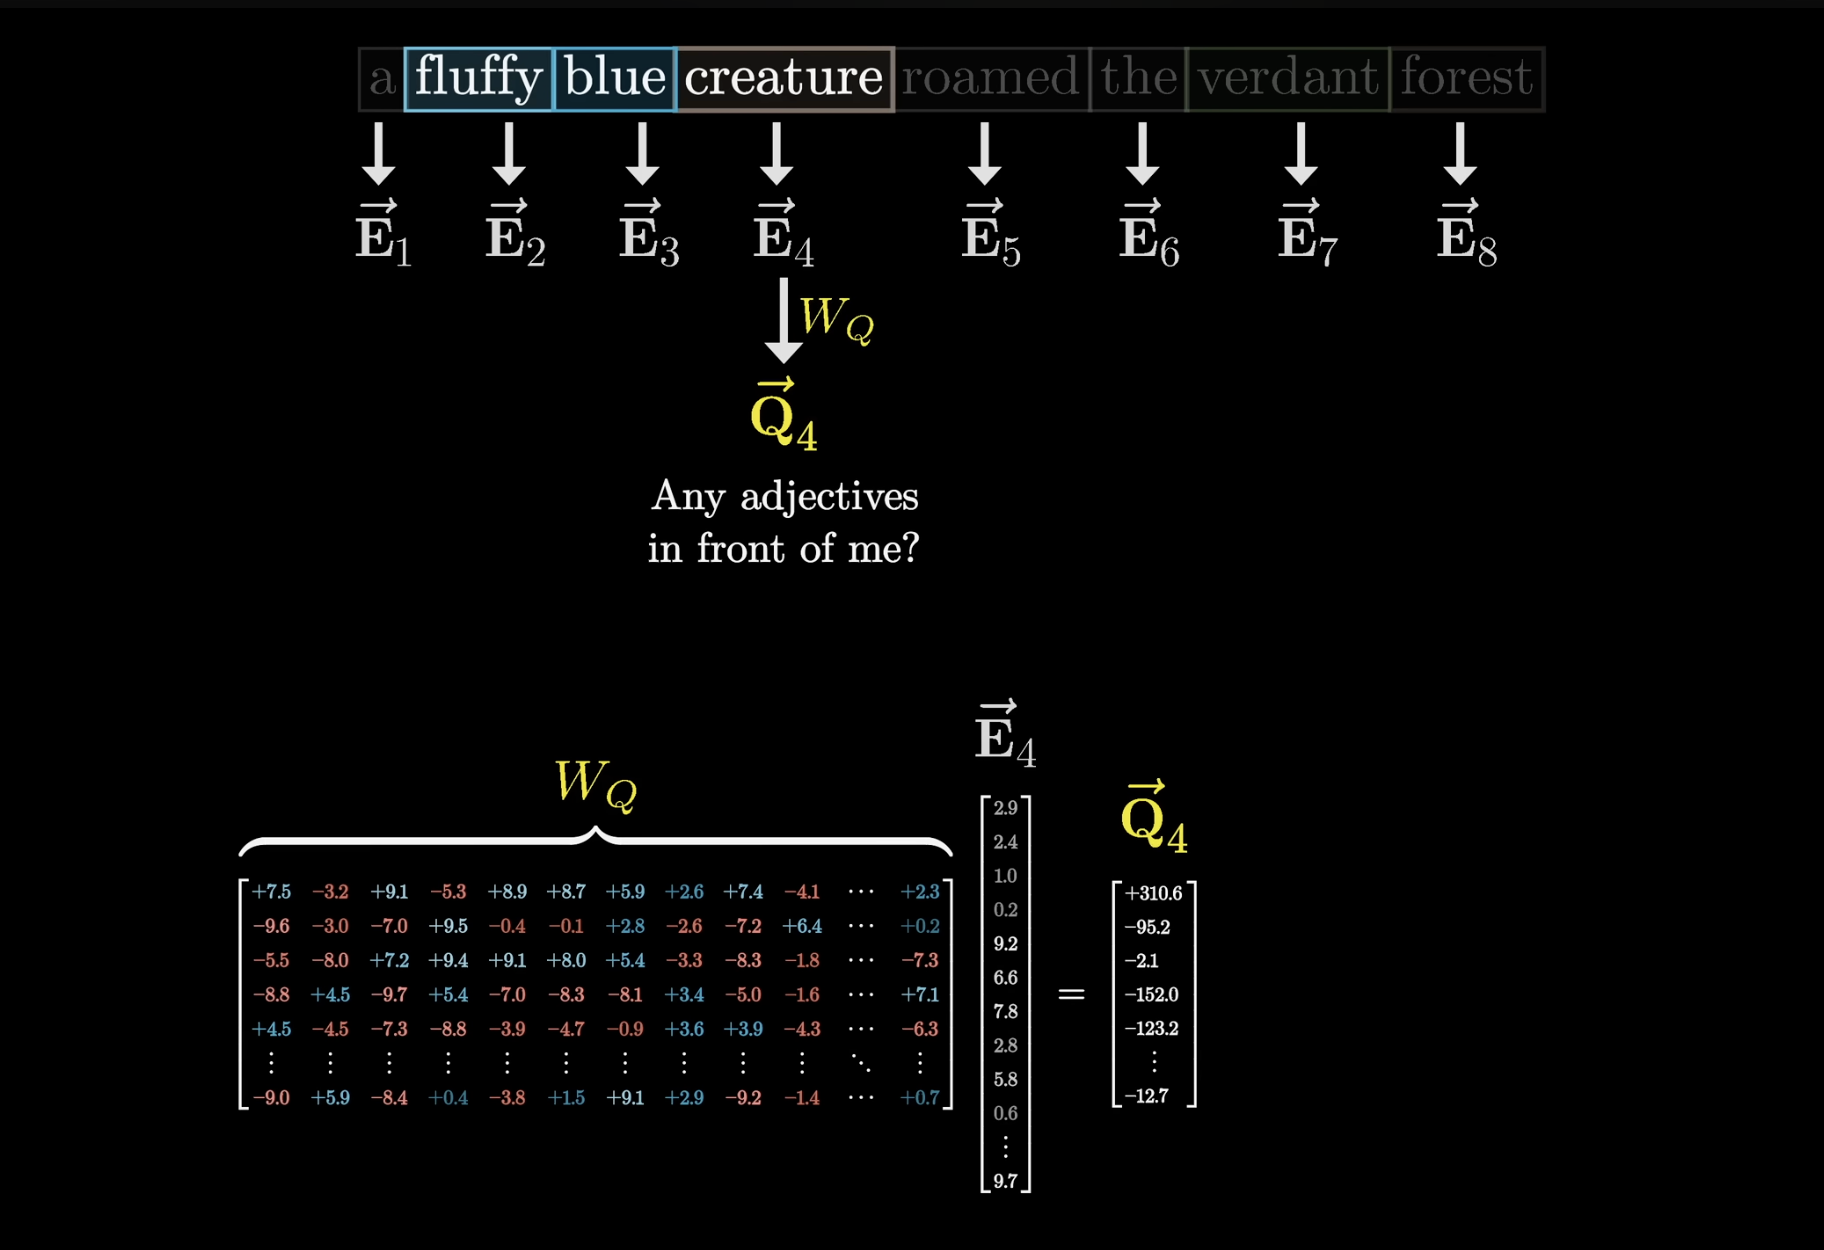
\includegraphics[width=0.85\textwidth]{images/query}}
\end{center}

\only<1-2>{
The question is encoded as another vector, called a \alert{query}, which is lower-dimensional
} 


\only<2>{
\begin{itemize}
\item How to get it? $\vec{Q}=\+W_Q \vec{E}$, where $\+W_Q$ is learnable.
\end{itemize}
}


\end{frame}



\begin{frame}{Single head of attention}

\begin{center}


\only<1->{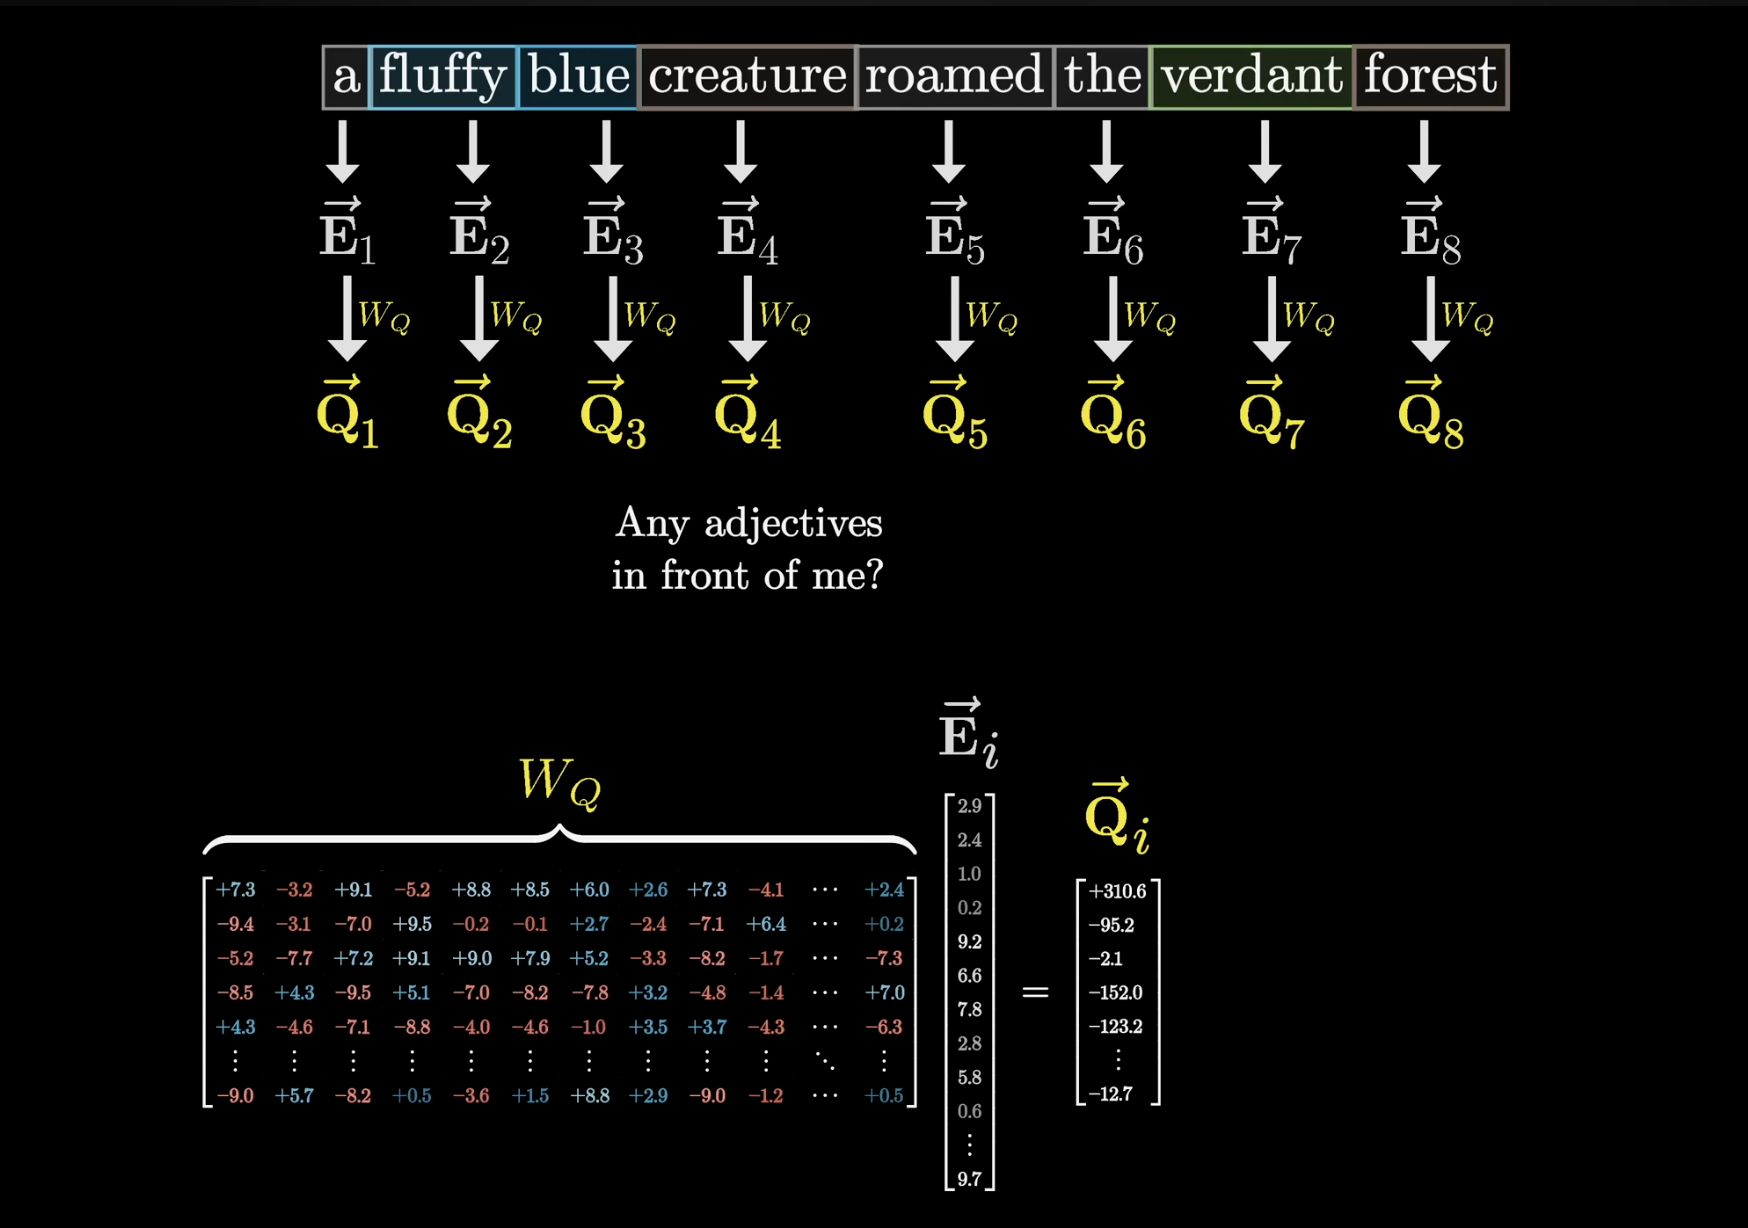
\includegraphics[width=0.85\textwidth]{images/queries}}

\only<1-2>{
We multiply this matrix by all the embeddings in the context.
} 


\only<2>{
This produces one query vector for each token.
}
\end{center}

\end{frame}



\begin{frame}{Single head of attention}

\begin{center}


\only<1->{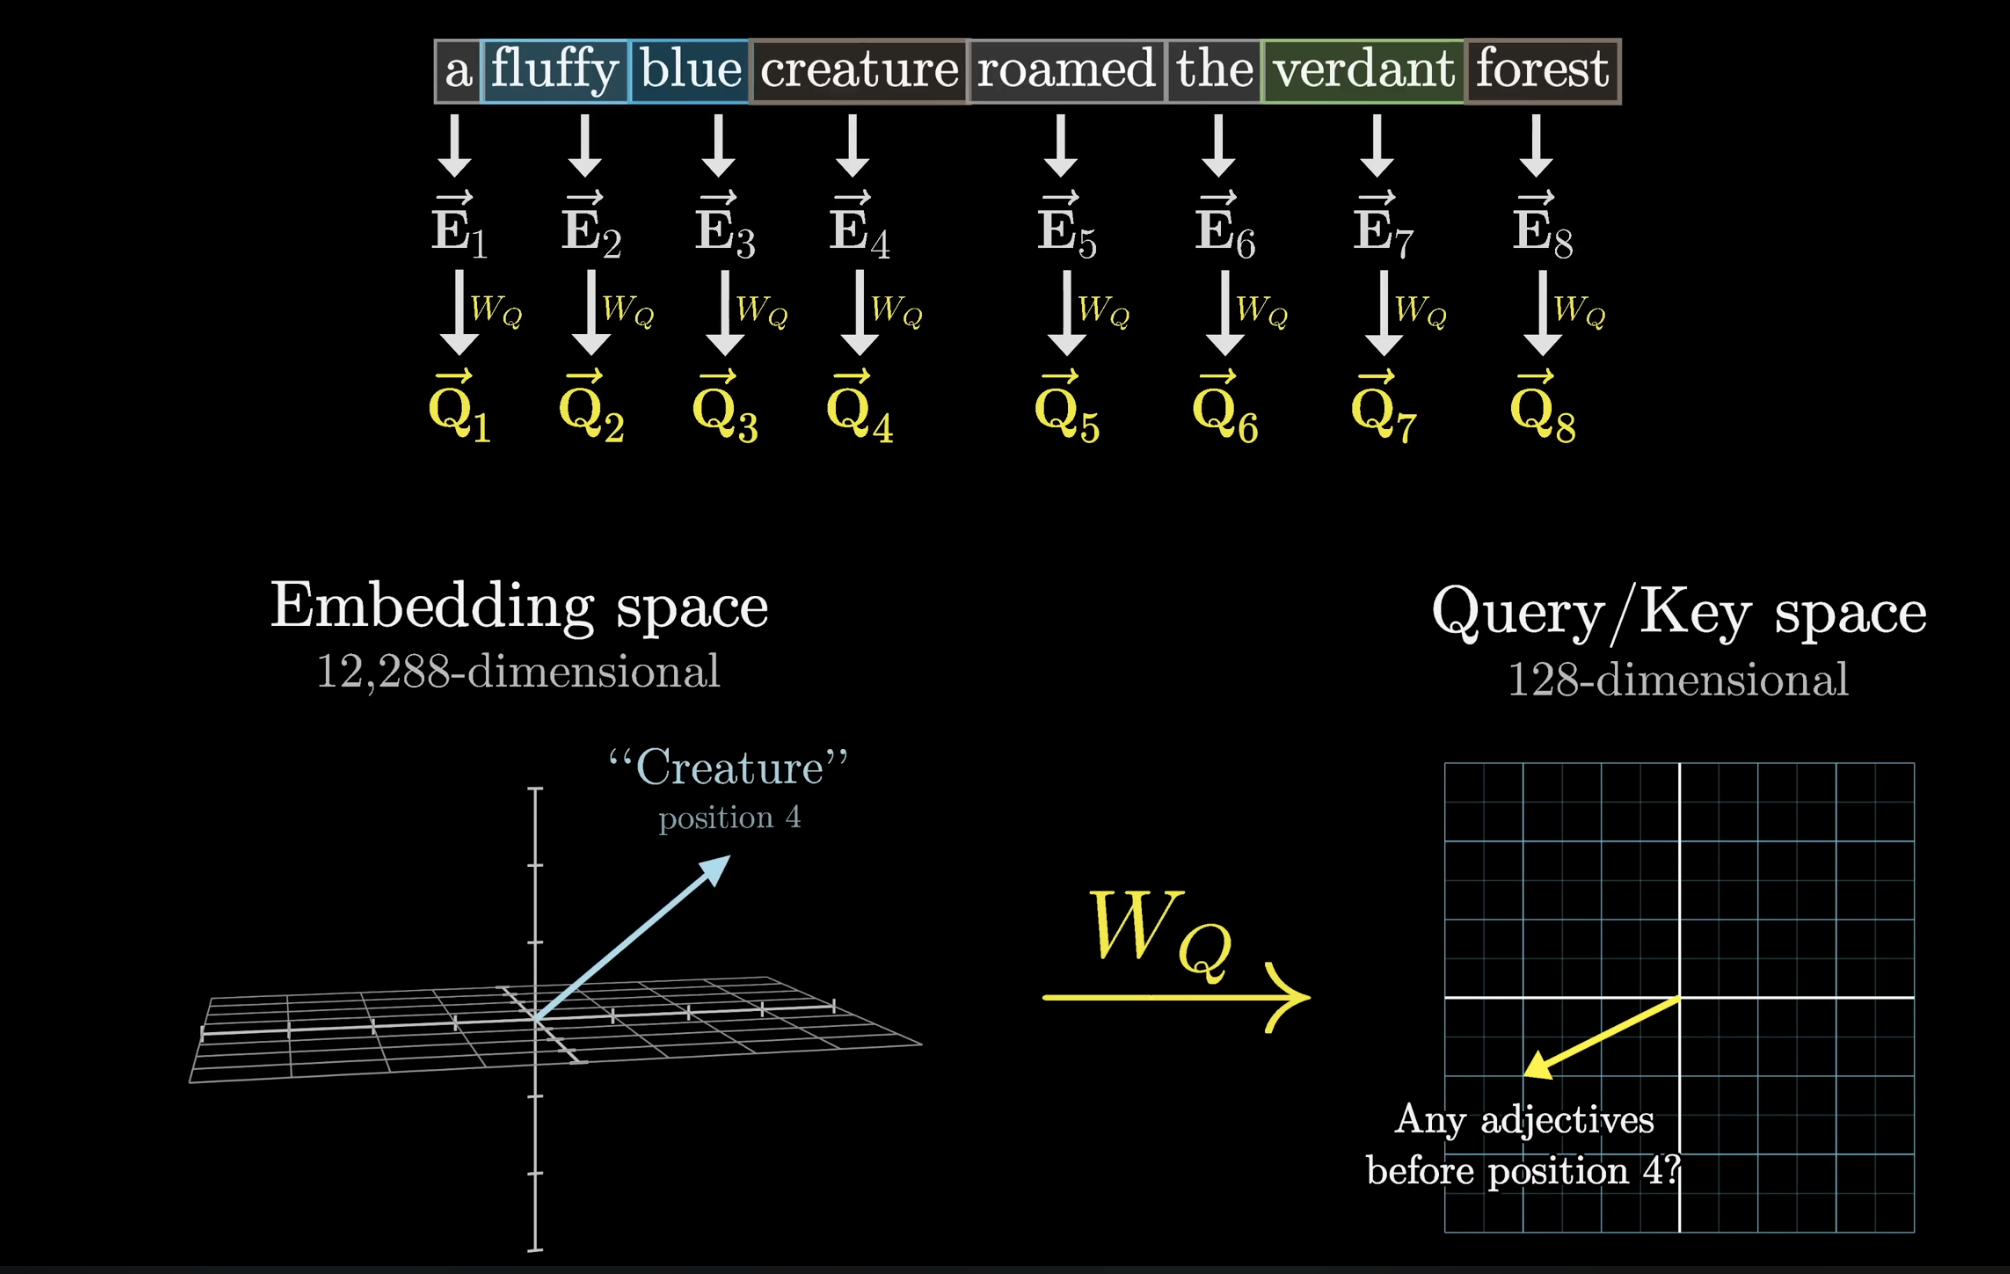
\includegraphics[width=0.85\textwidth]{images/query_matrix}}

\only<1->{
We'll hope this \alert{query matrix} maps the embeddings of nouns to certain directions in this smaller query space that encodes the notion of looking for adjectives in preceding positions.
} 


\end{center}

\end{frame}


\begin{frame}{Single head of attention}

\begin{center}


\only<1-2>{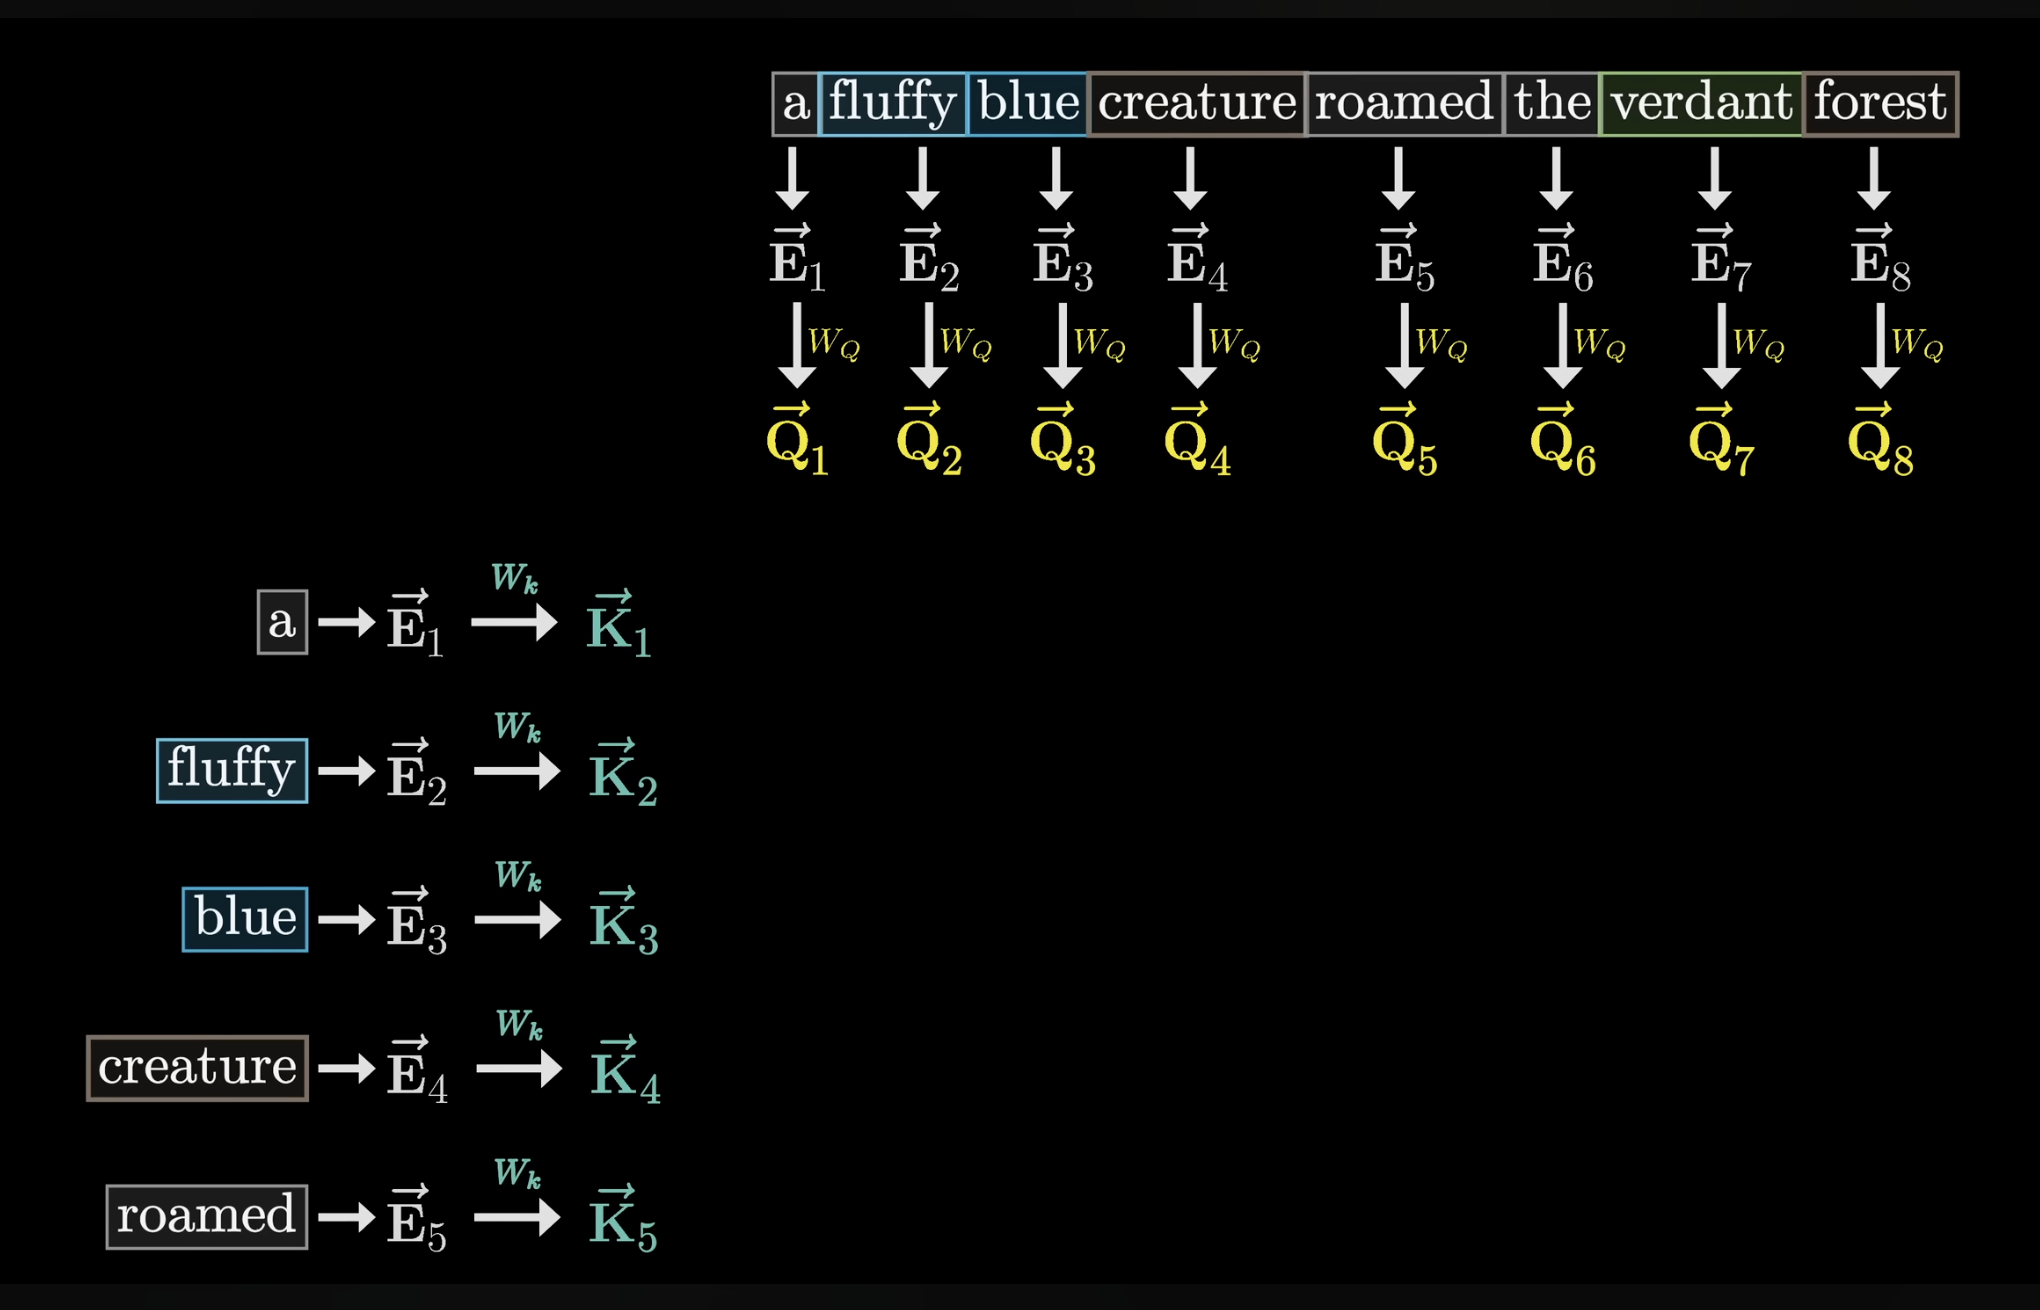
\includegraphics[width=0.85\textwidth]{images/key_matrix}}

\only<3>{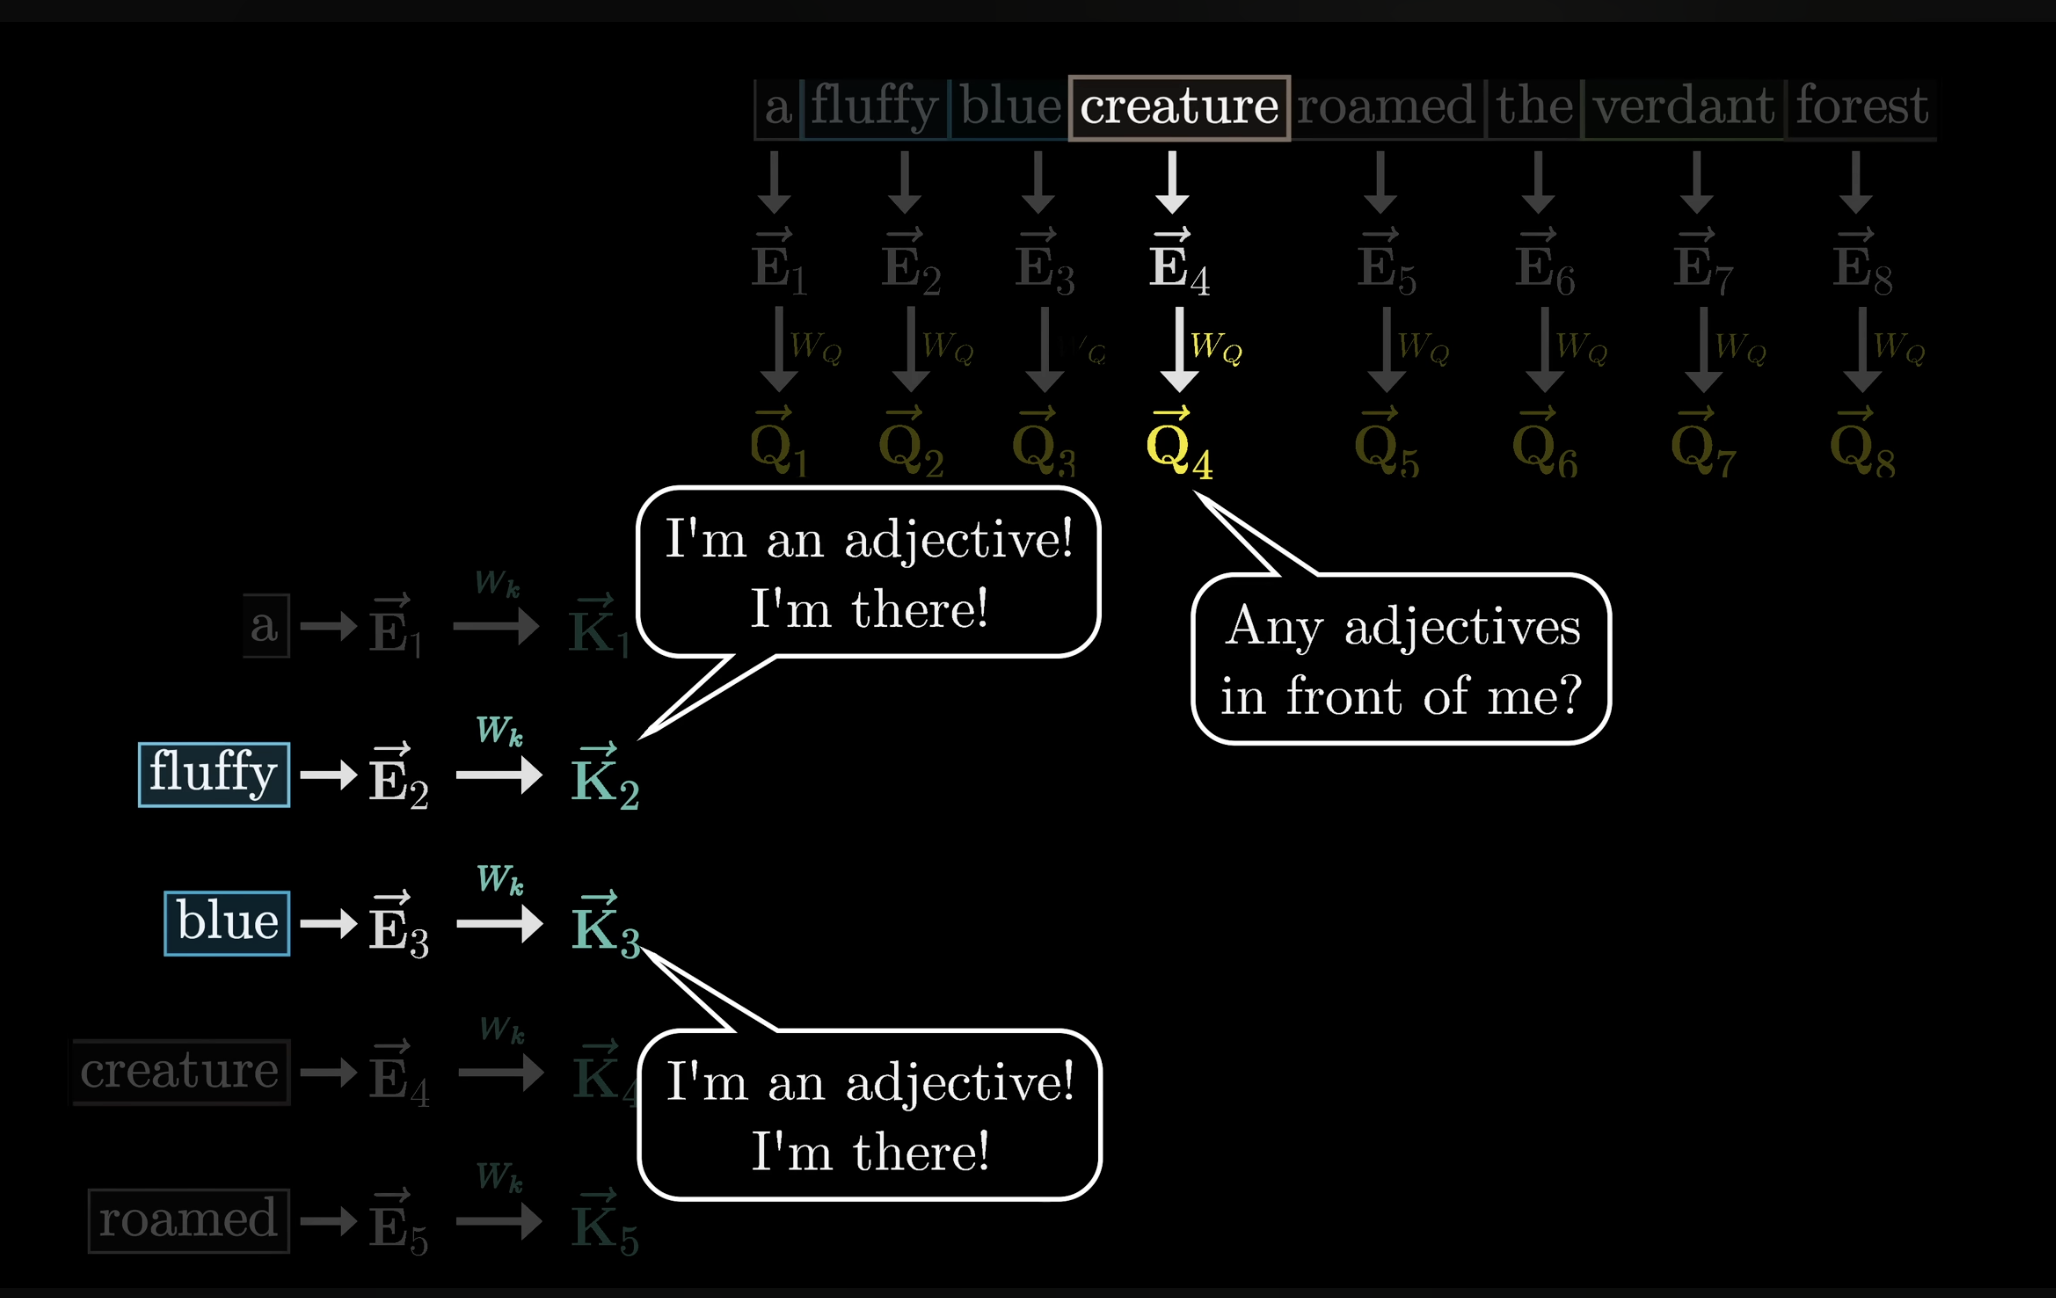
\includegraphics[width=0.85\textwidth]{images/answer_queries}}

\only<4->{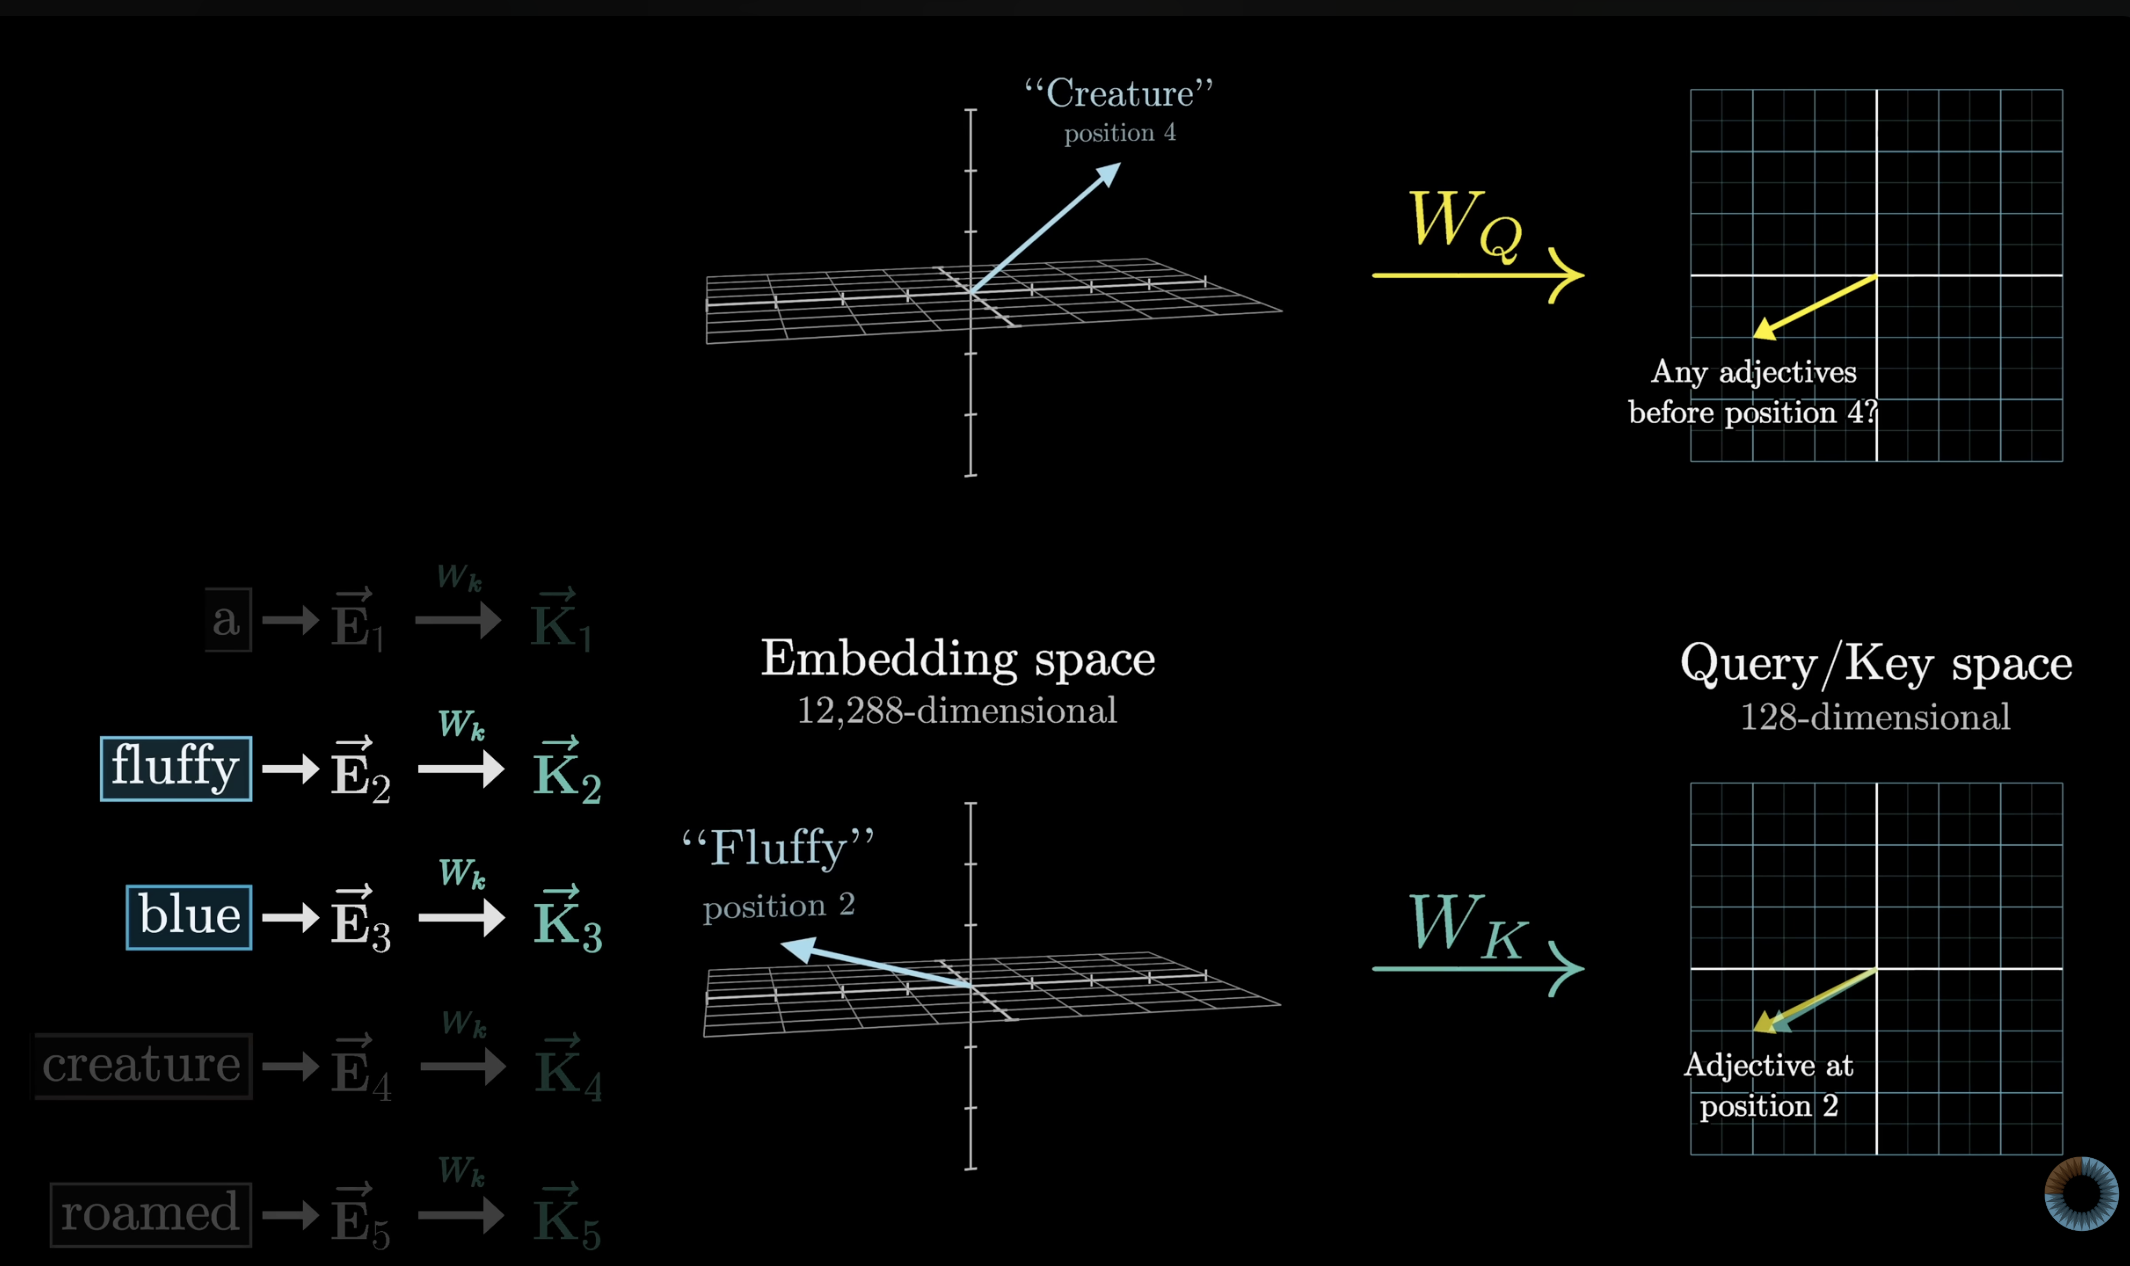
\includegraphics[width=0.85\textwidth]{images/key_space}}


\end{center}


\only<1-2>{
A second matrix, called the \alert{key matrix}, transforms the same embeddings into a sequence of \textbf{key vectors}.
} 

\only<2>{
\begin{itemize}
\item How to get it? $\vec{K}=\+W_K \vec{E}$, where $\+W_K$ is learnable.
\end{itemize}
}



\only<3>{
Think of the keys as potentially \alert{answering} the queries.
} 

\only<4>{
The key matrix maps the embeddings to the same lower dimensional space as the query matrix.
} 

\only<5>{
Think of keys as matching the queries when they closely align.
} 

\only<6>{
Here, adjectives like \qq{fluffy} and \qq{blue} get mapped to similar directions as the query produced by the word \qq{creature}.
} 



\end{frame}



\begin{frame}{Single head of attention}

\begin{center}
\only<1>{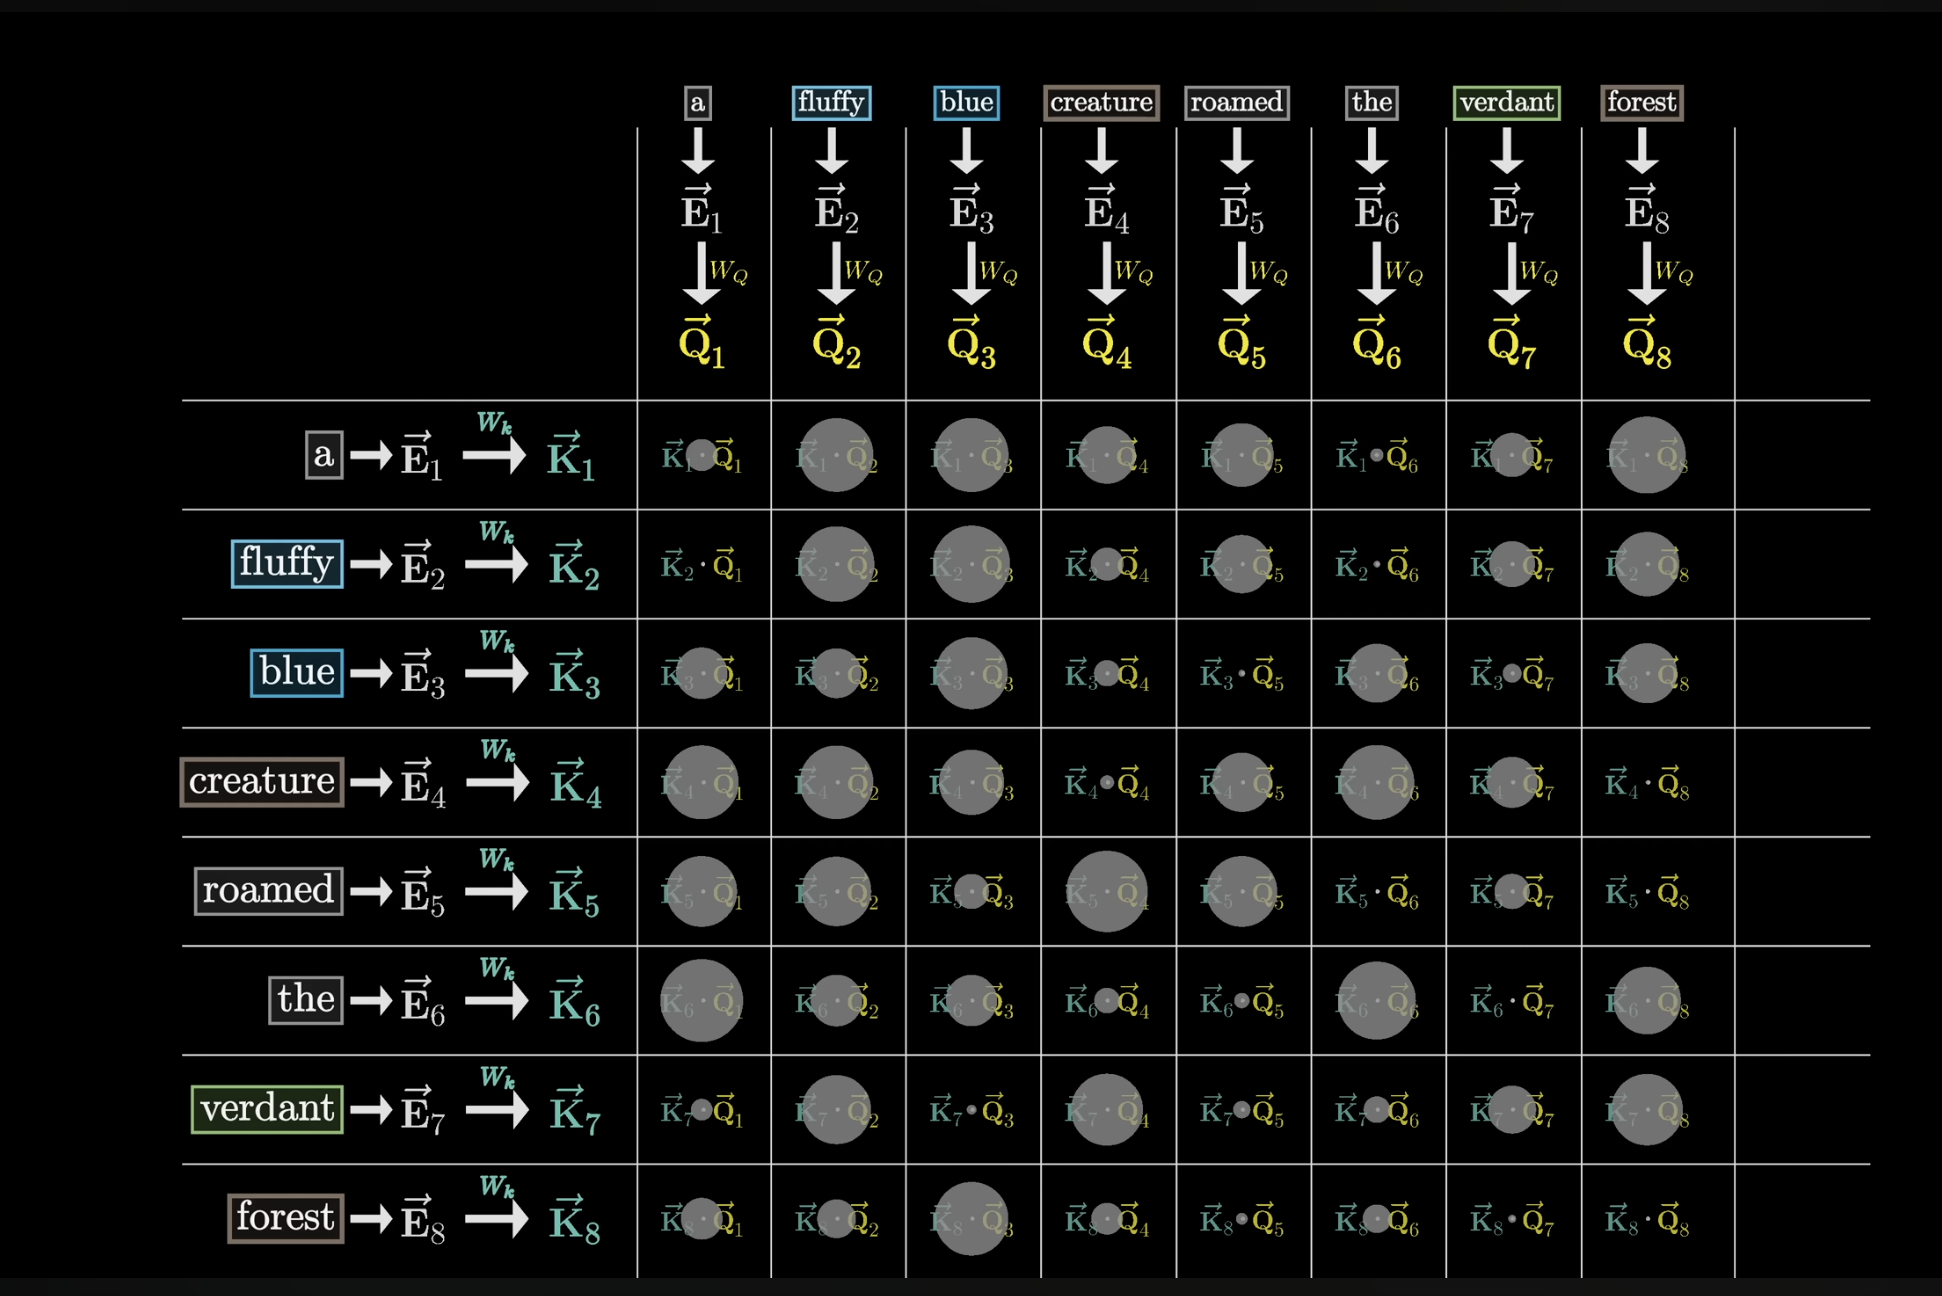
\includegraphics[width=0.85\textwidth]{images/dot_product1}}
\only<2>{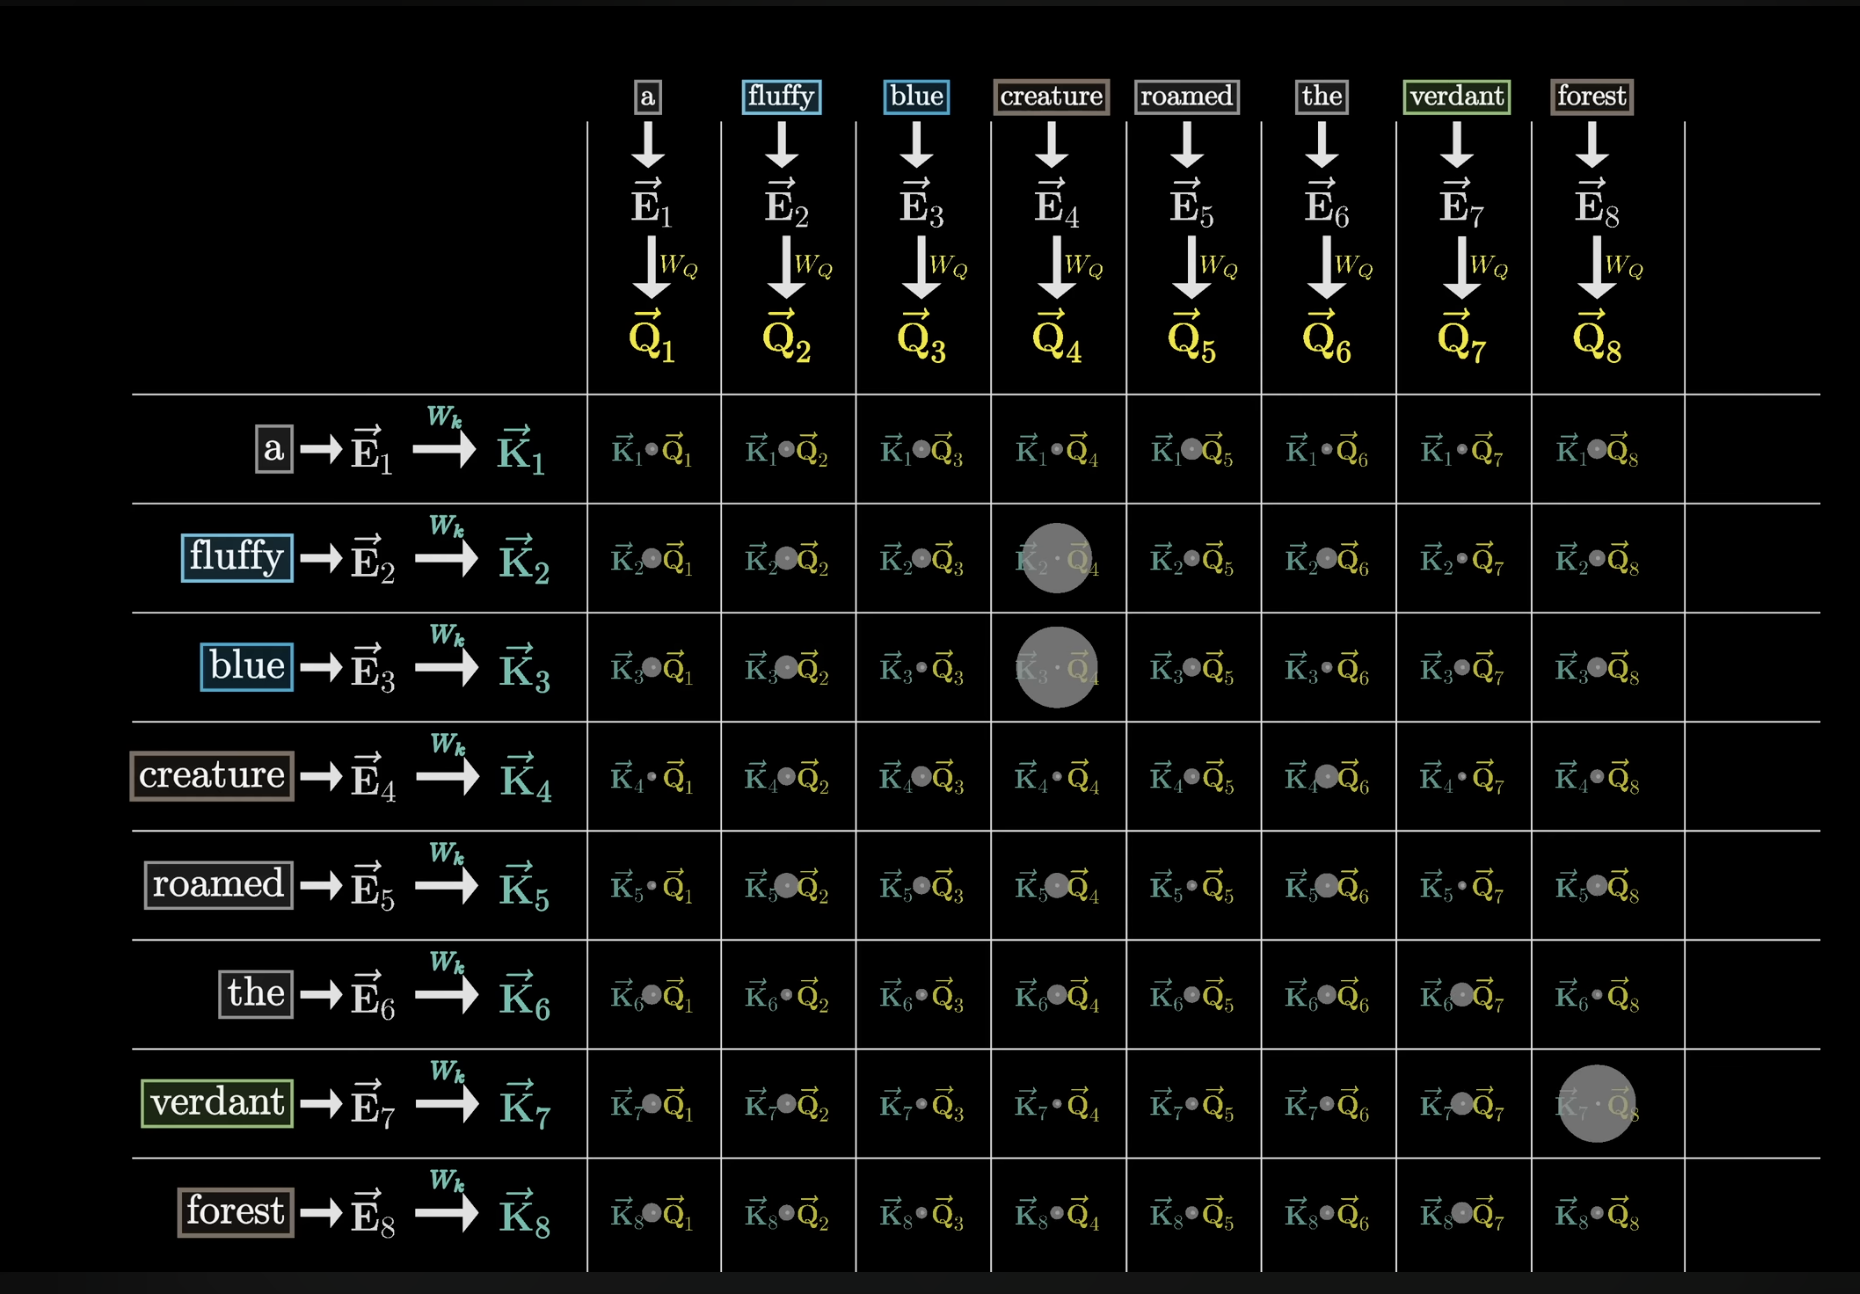
\includegraphics[width=0.85\textwidth]{images/dot_product2}}
\only<3-4>{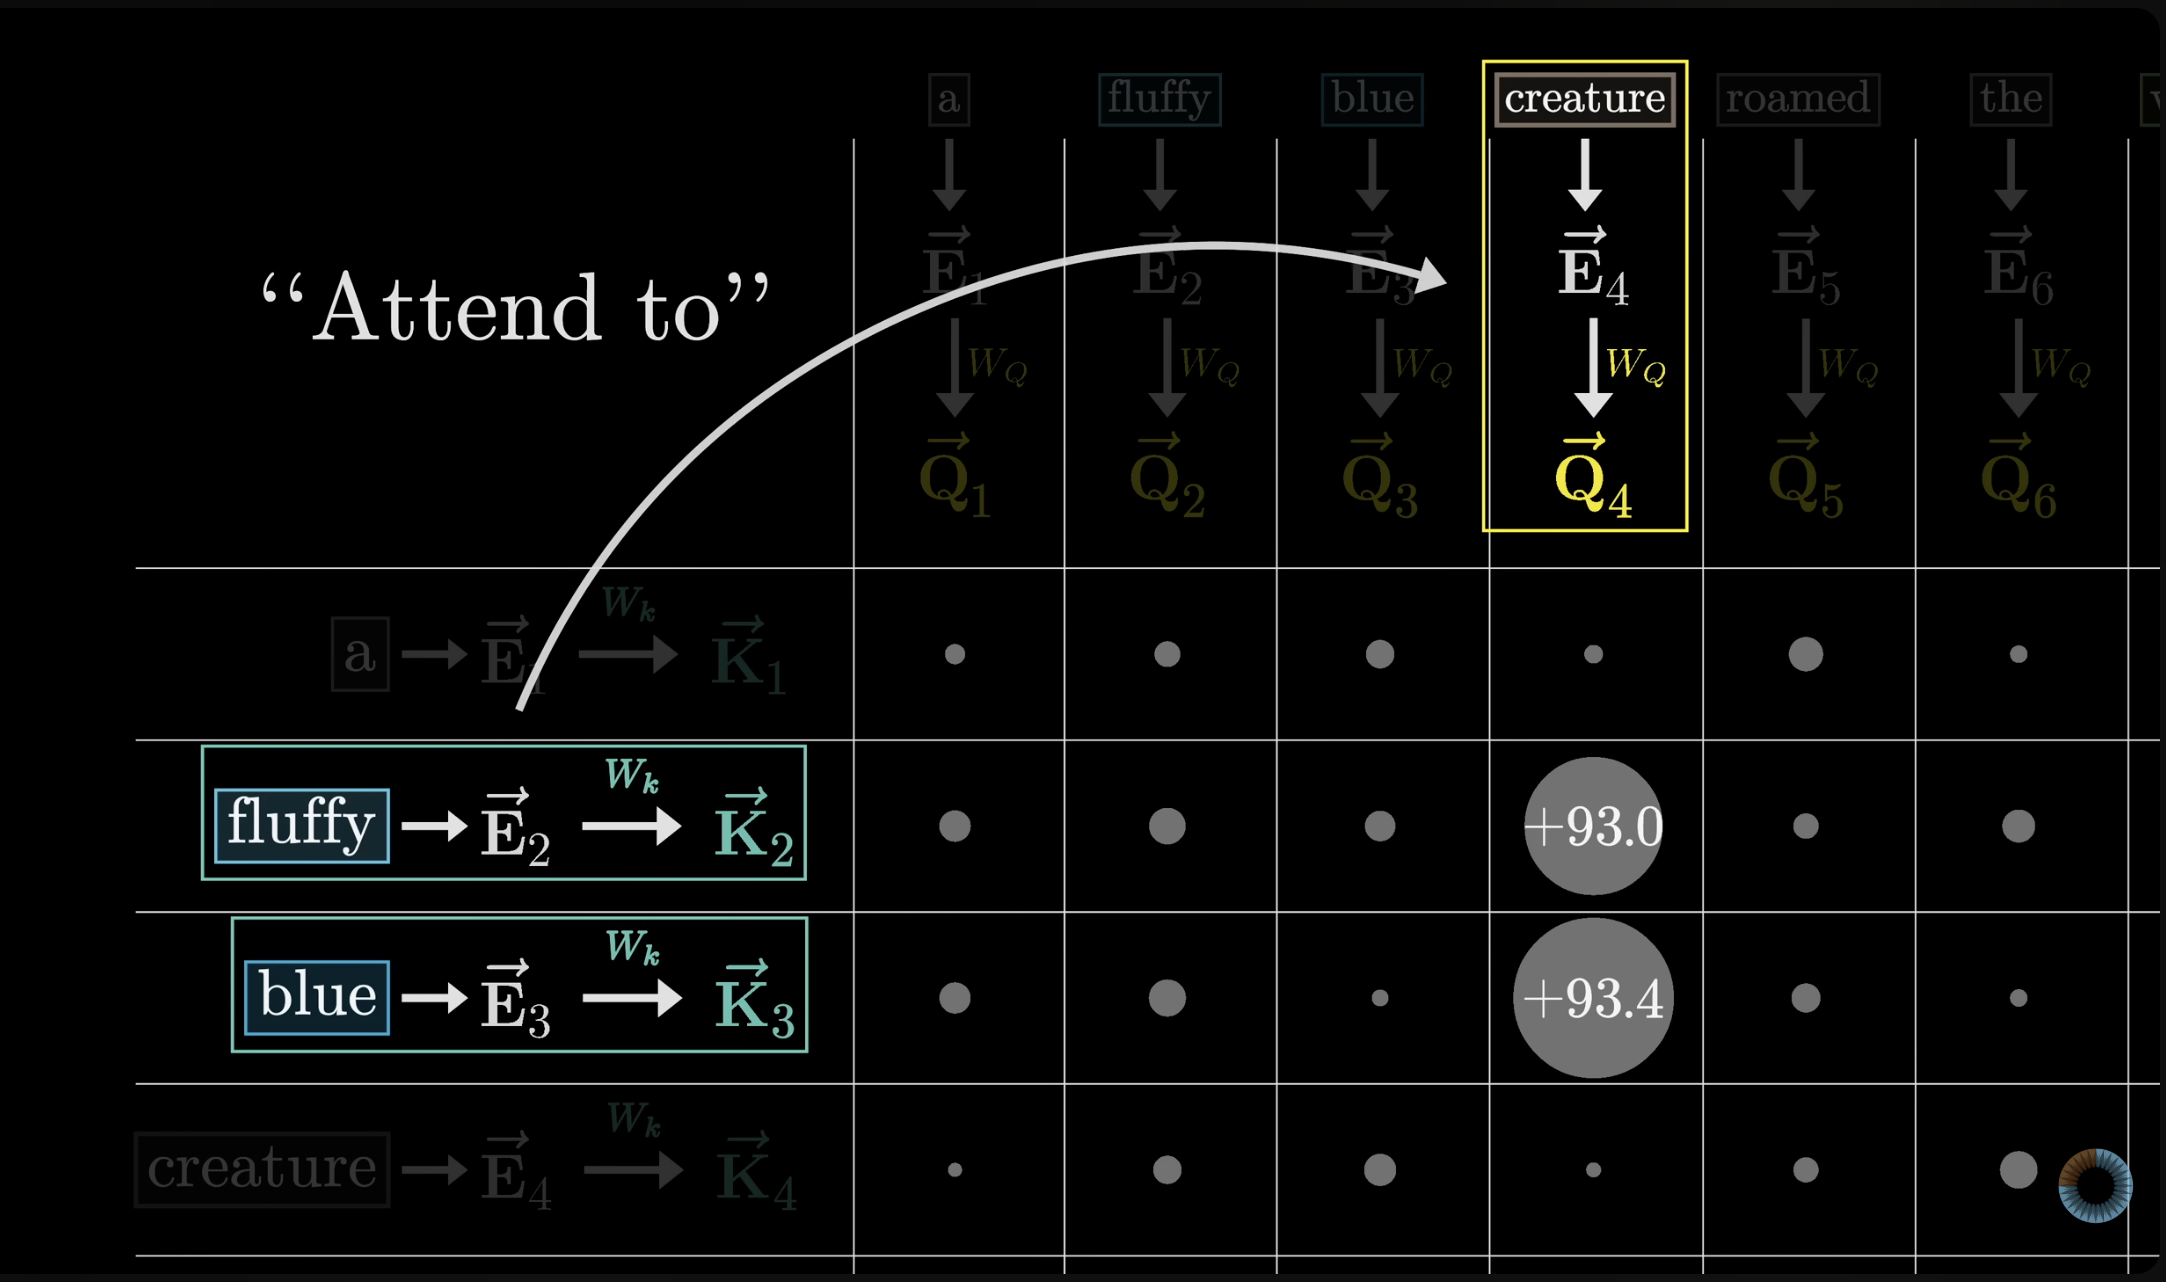
\includegraphics[width=0.85\textwidth]{images/attend_to}}
\only<5>{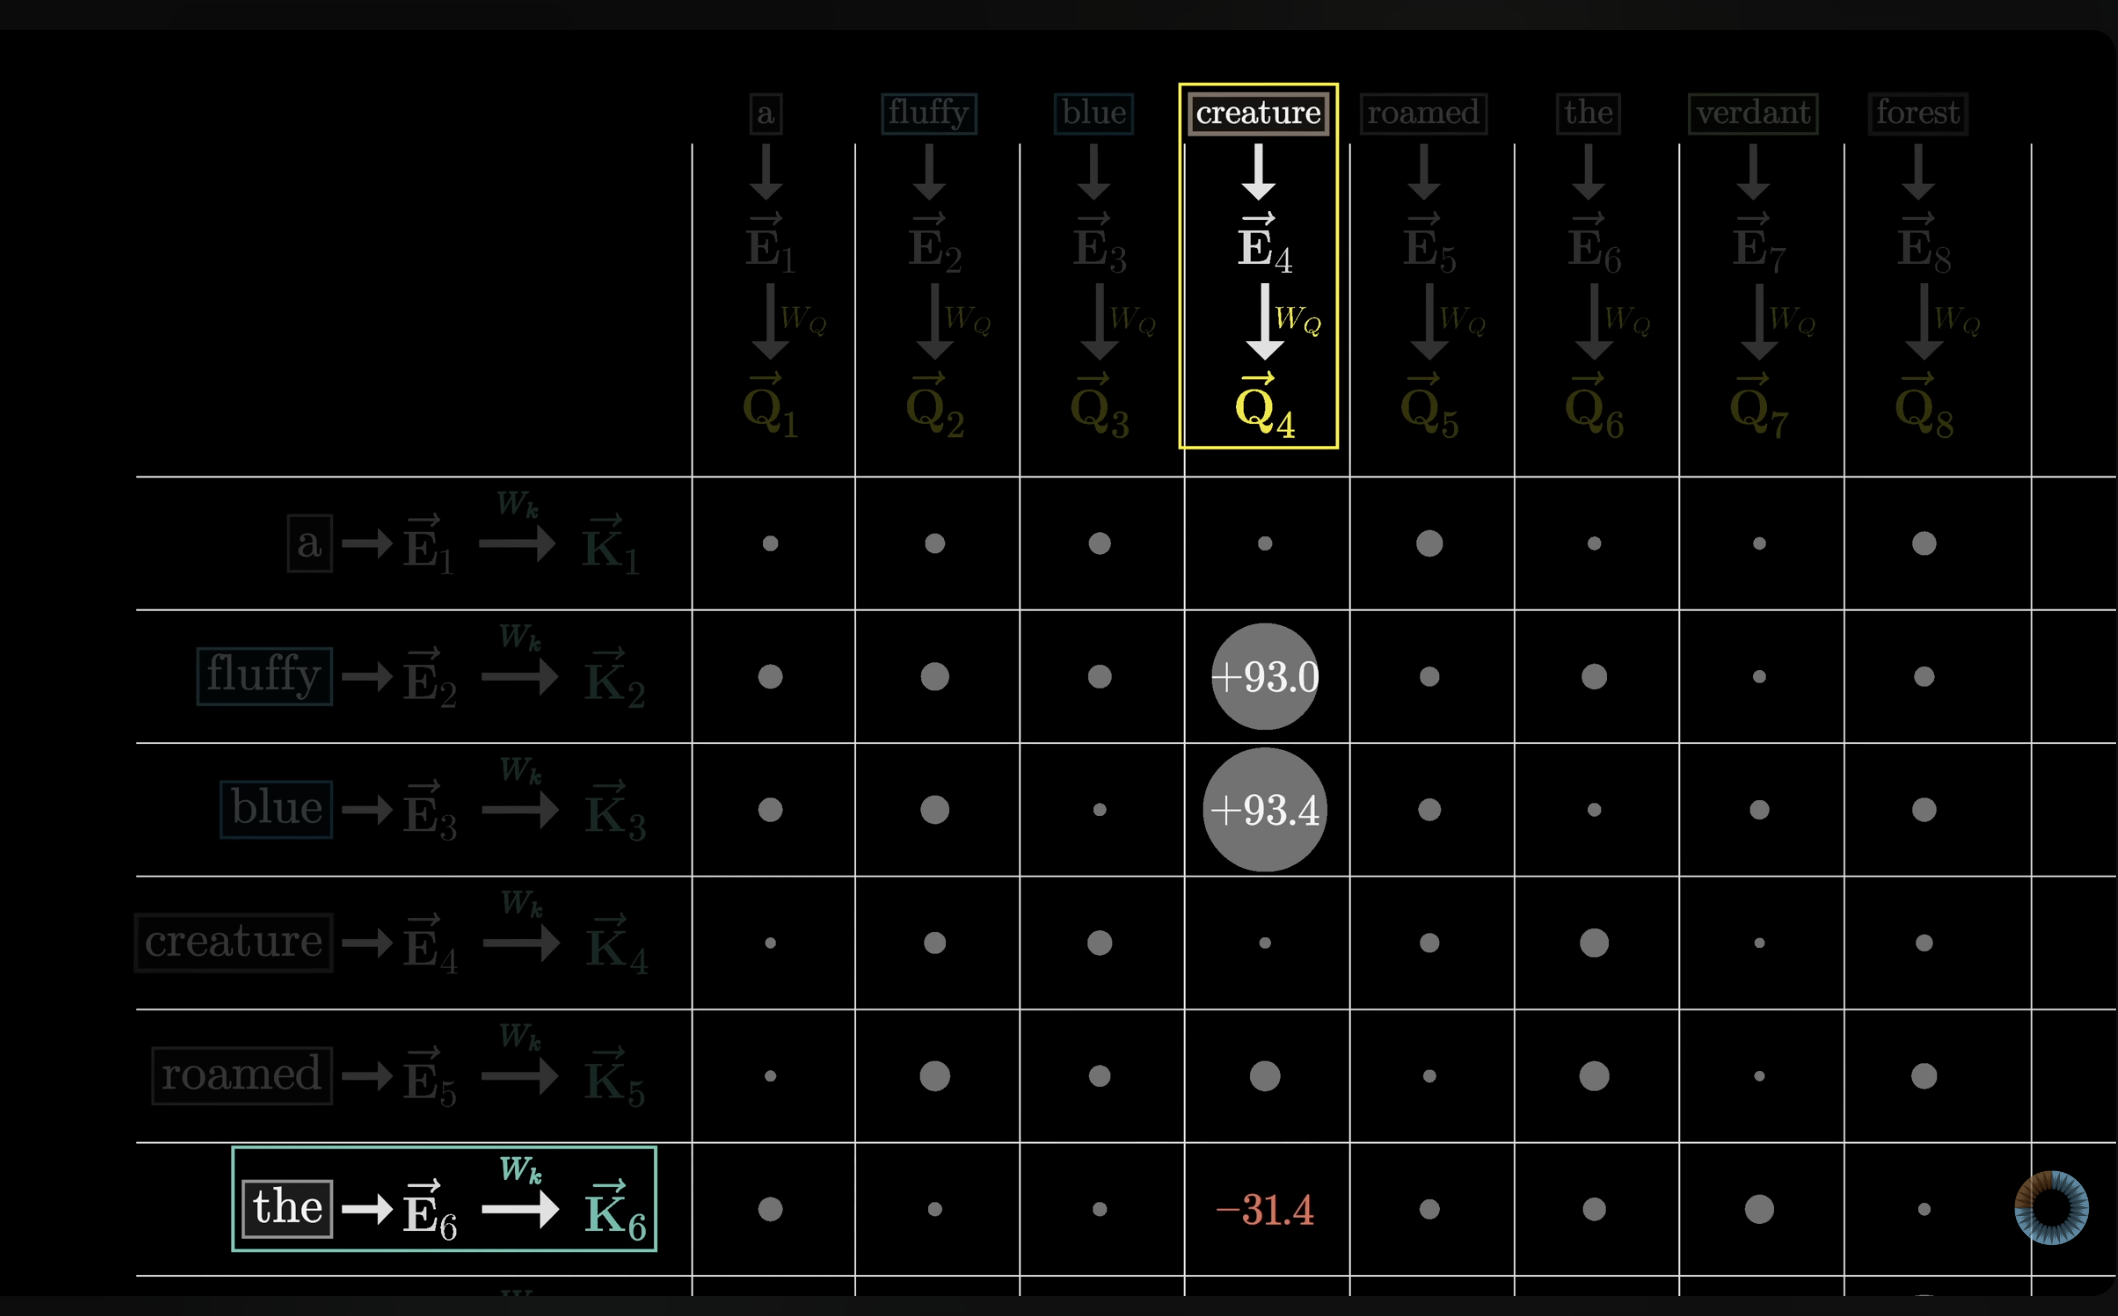
\includegraphics[width=0.85\textwidth]{images/dot_product3}}

\only<1-2>{
To measure how well keys and queries align, compute the dot product
\[  \vec{K_i} \cdot \vec{Q_j}, \qquad \qquad \text{ also written as } \vec{K_i}^\top \vec{Q_j} \]
} 

\only<3>{Here the dot product is large and positive.}

\only<4>{ We say the embeddings for \qq{fluffy} and \qq{blue} \alert{attend} to the embedding for \qq{creature}.
}

\only<5>{Dot products with words unrelated to the query will be small or negative.
}
\end{center}

\end{frame}


\begin{frame}{Single head of attention}

\begin{center}
\only<1-2>{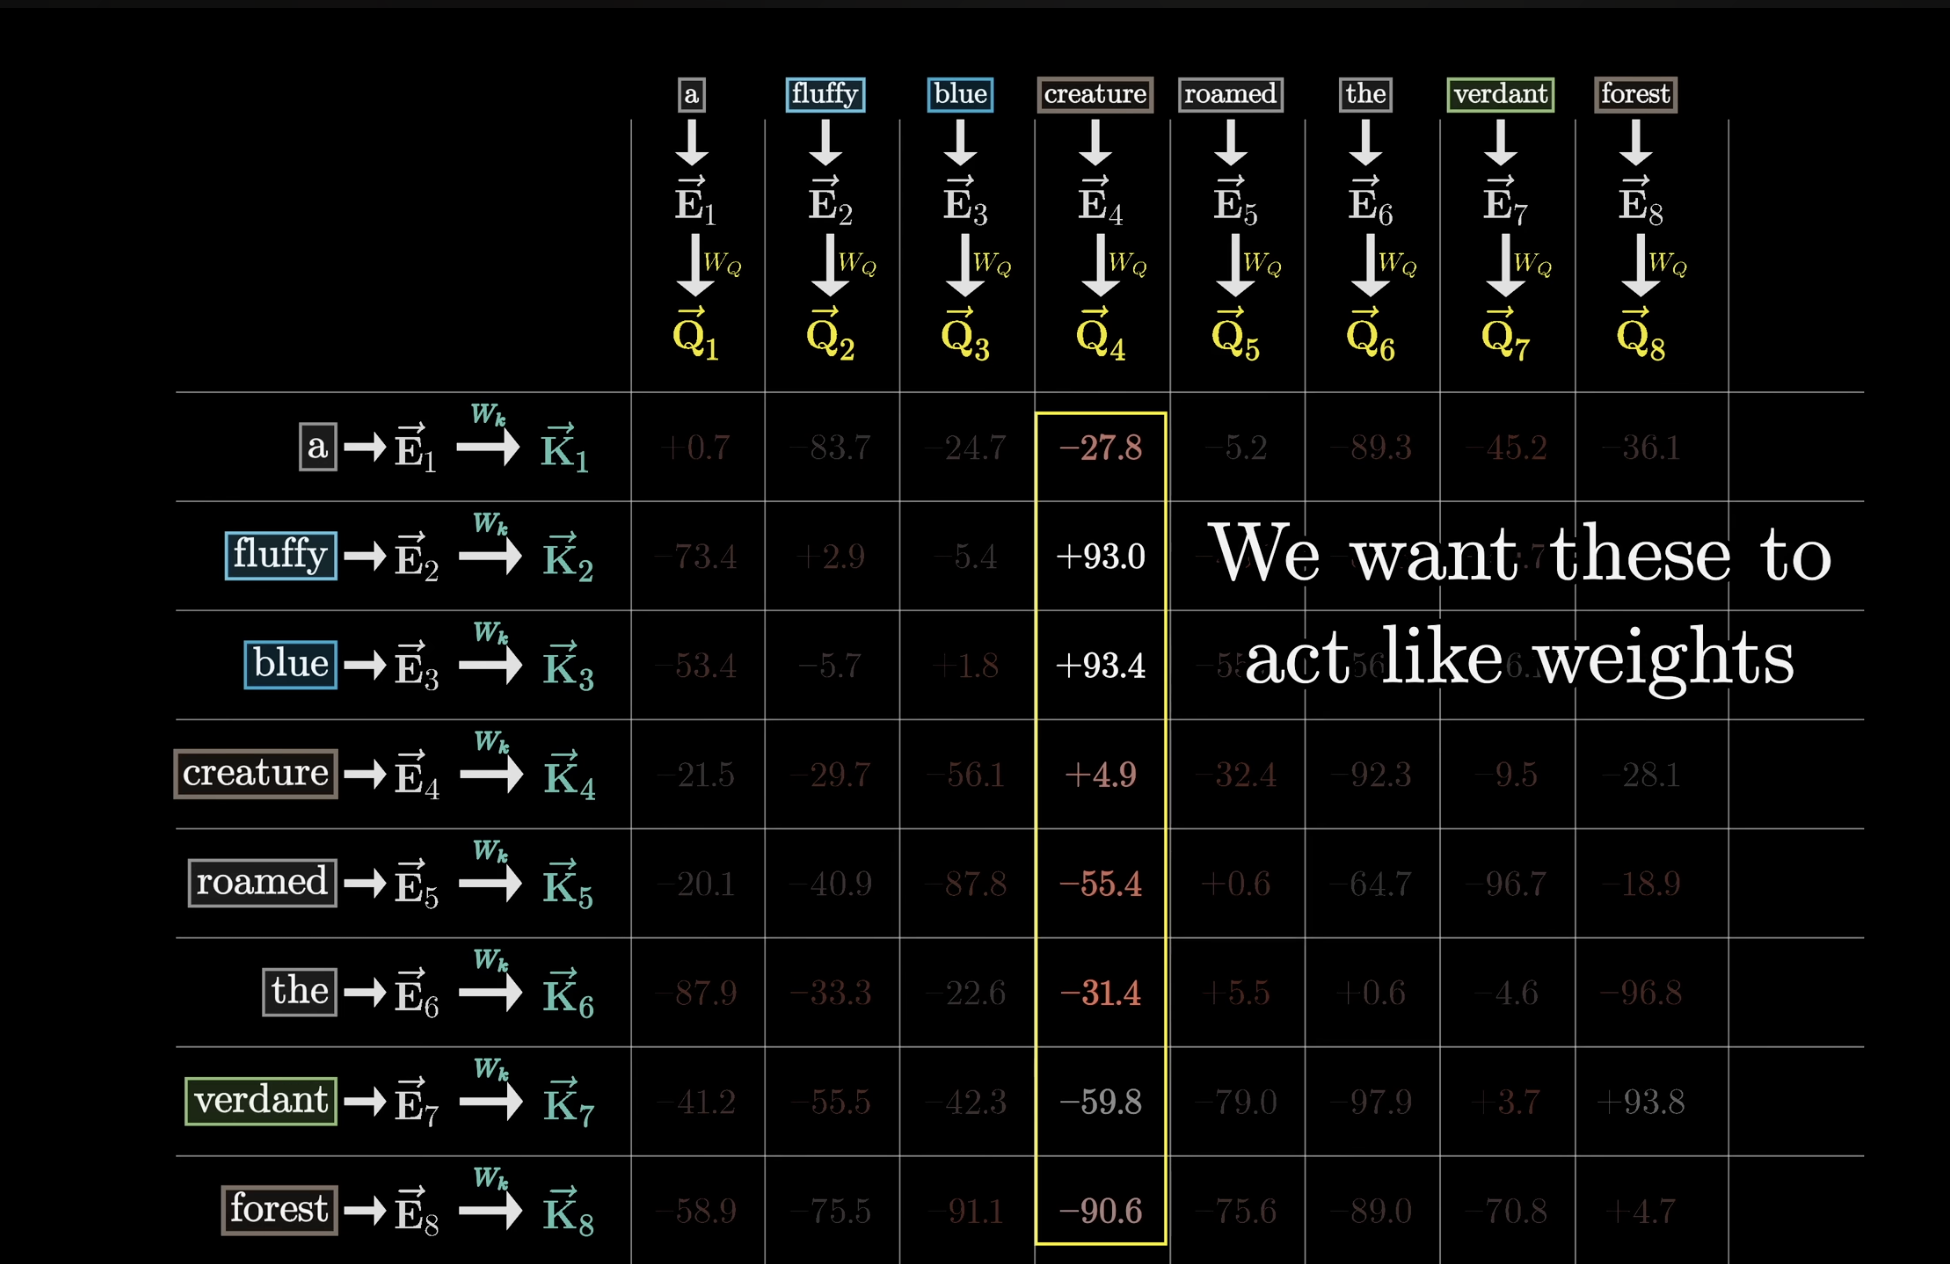
\includegraphics[width=0.85\textwidth]{images/dot_products_raw}}
\only<3>{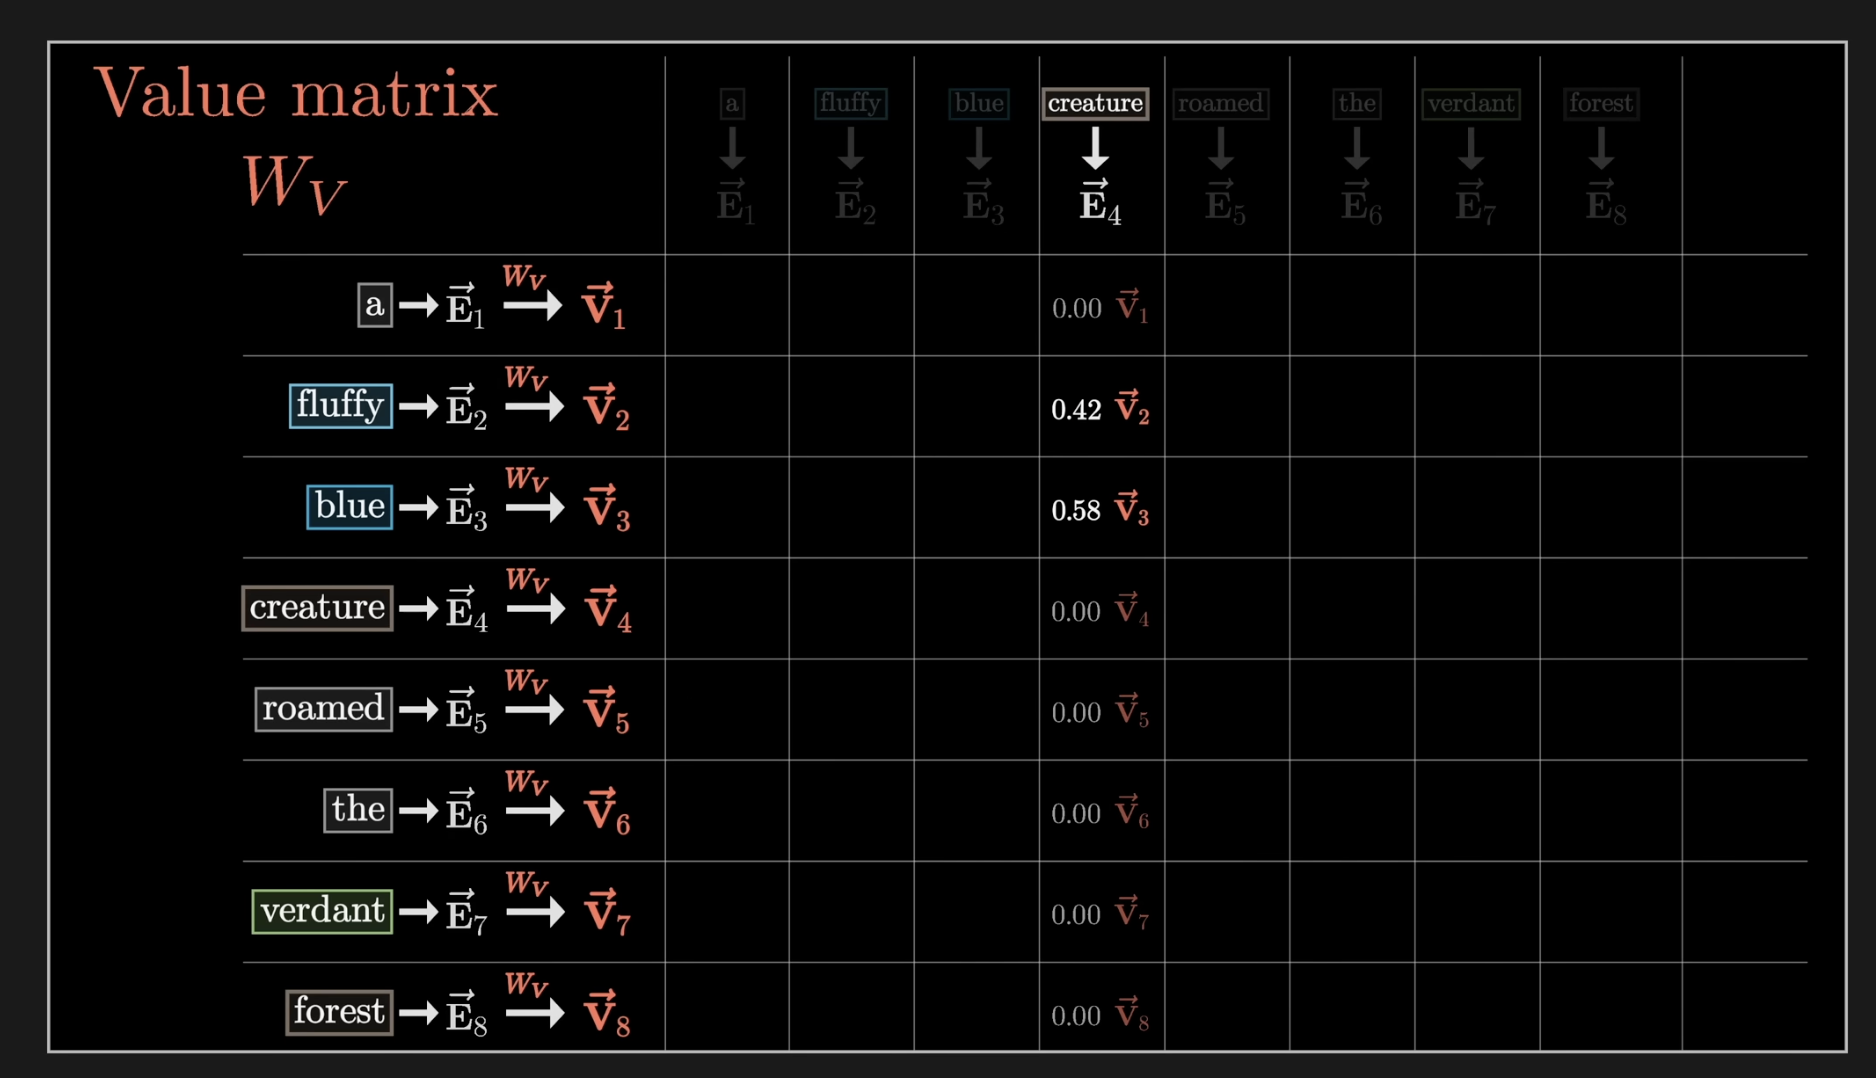
\includegraphics[width=0.85\textwidth]{images/dot_products_normalized}}
\only<4-5>{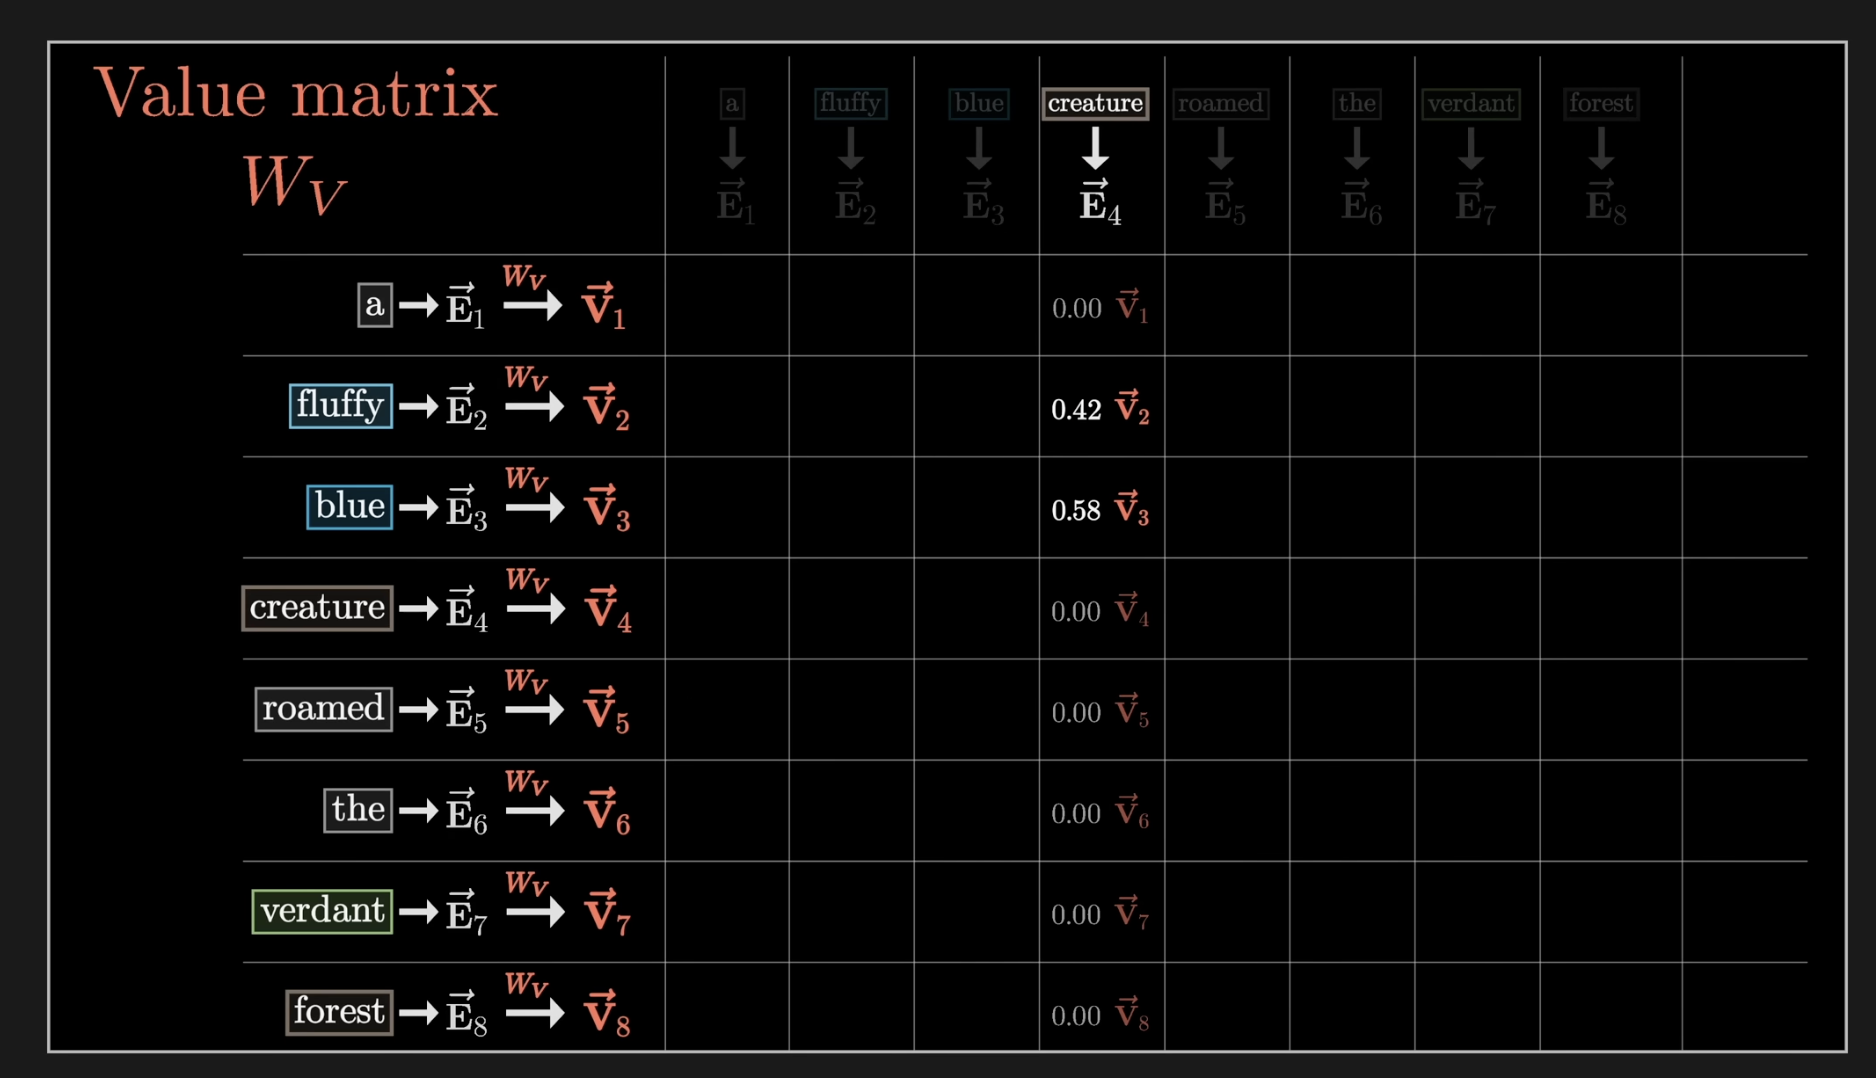
\includegraphics[width=0.60\textwidth]{images/dot_products_normalized}}
\end{center}

\only<1-2>{
The raw dot products are real numbers in $(-\infty, \infty)$.
} 
\only<2>{These score how relevant each word is for updating the meaning of each other word.
} 

\only<3-5>{
We want to \alert{normalize} these dot products to act like probability weights along each column.
} 

\only<4>{So we apply the \textbf{softmax} function

\[ \alpha_{ji}=\frac{\exp\left(\frac{K_i^\top Q_j}{\sqrt{d}}\right)}{\sum_{i'} \exp\left(\frac{K_{i'}^\top Q_j}{\sqrt{d}}\right)} \]
where $d$ is the dimension of key/query space. 
}

\only<5>{In matrix form
\[
\mathrm{softmax}\left(\frac{\+K^\top\+Q}{\sqrt{d}}\right)\]

The softmax is applied \textbf{row-wise} (across keys for each query).
} 

\end{frame}


\begin{frame}{Single head of attention}

\begin{center}
\only<1-2>{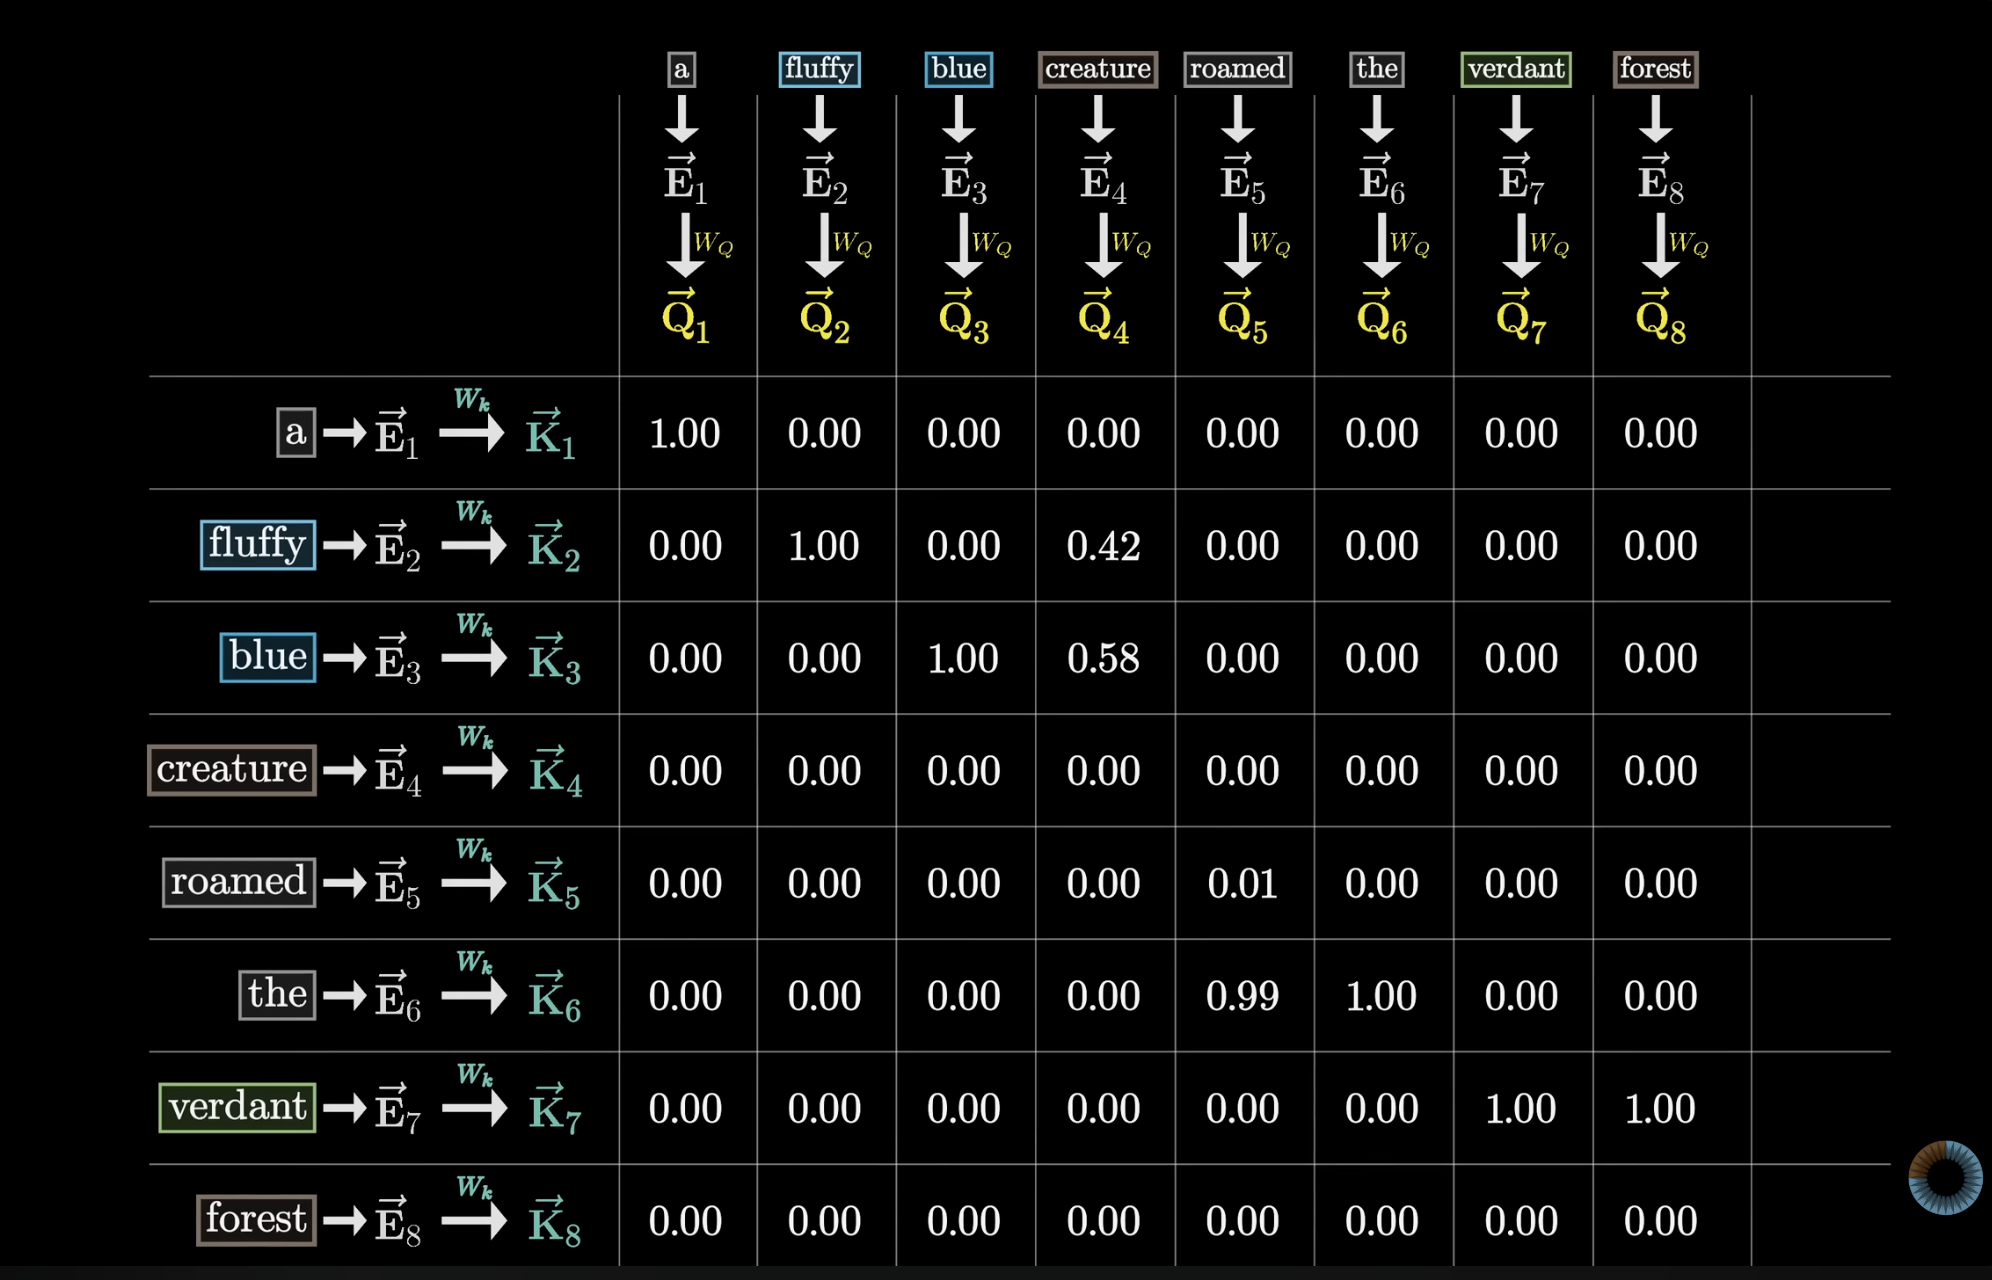
\includegraphics[width=0.85\textwidth]{images/attention_pattern}}
\end{center}

\only<1-2>{
After normalization, the grid gives weights telling us how relevant each word on the left is to the corresponding word on the top.
}  \only<2>{We call this grid an \alert{attention pattern}.} 

\end{frame}



\begin{frame}{Causal masking}
\begin{center}
\only<1-2>{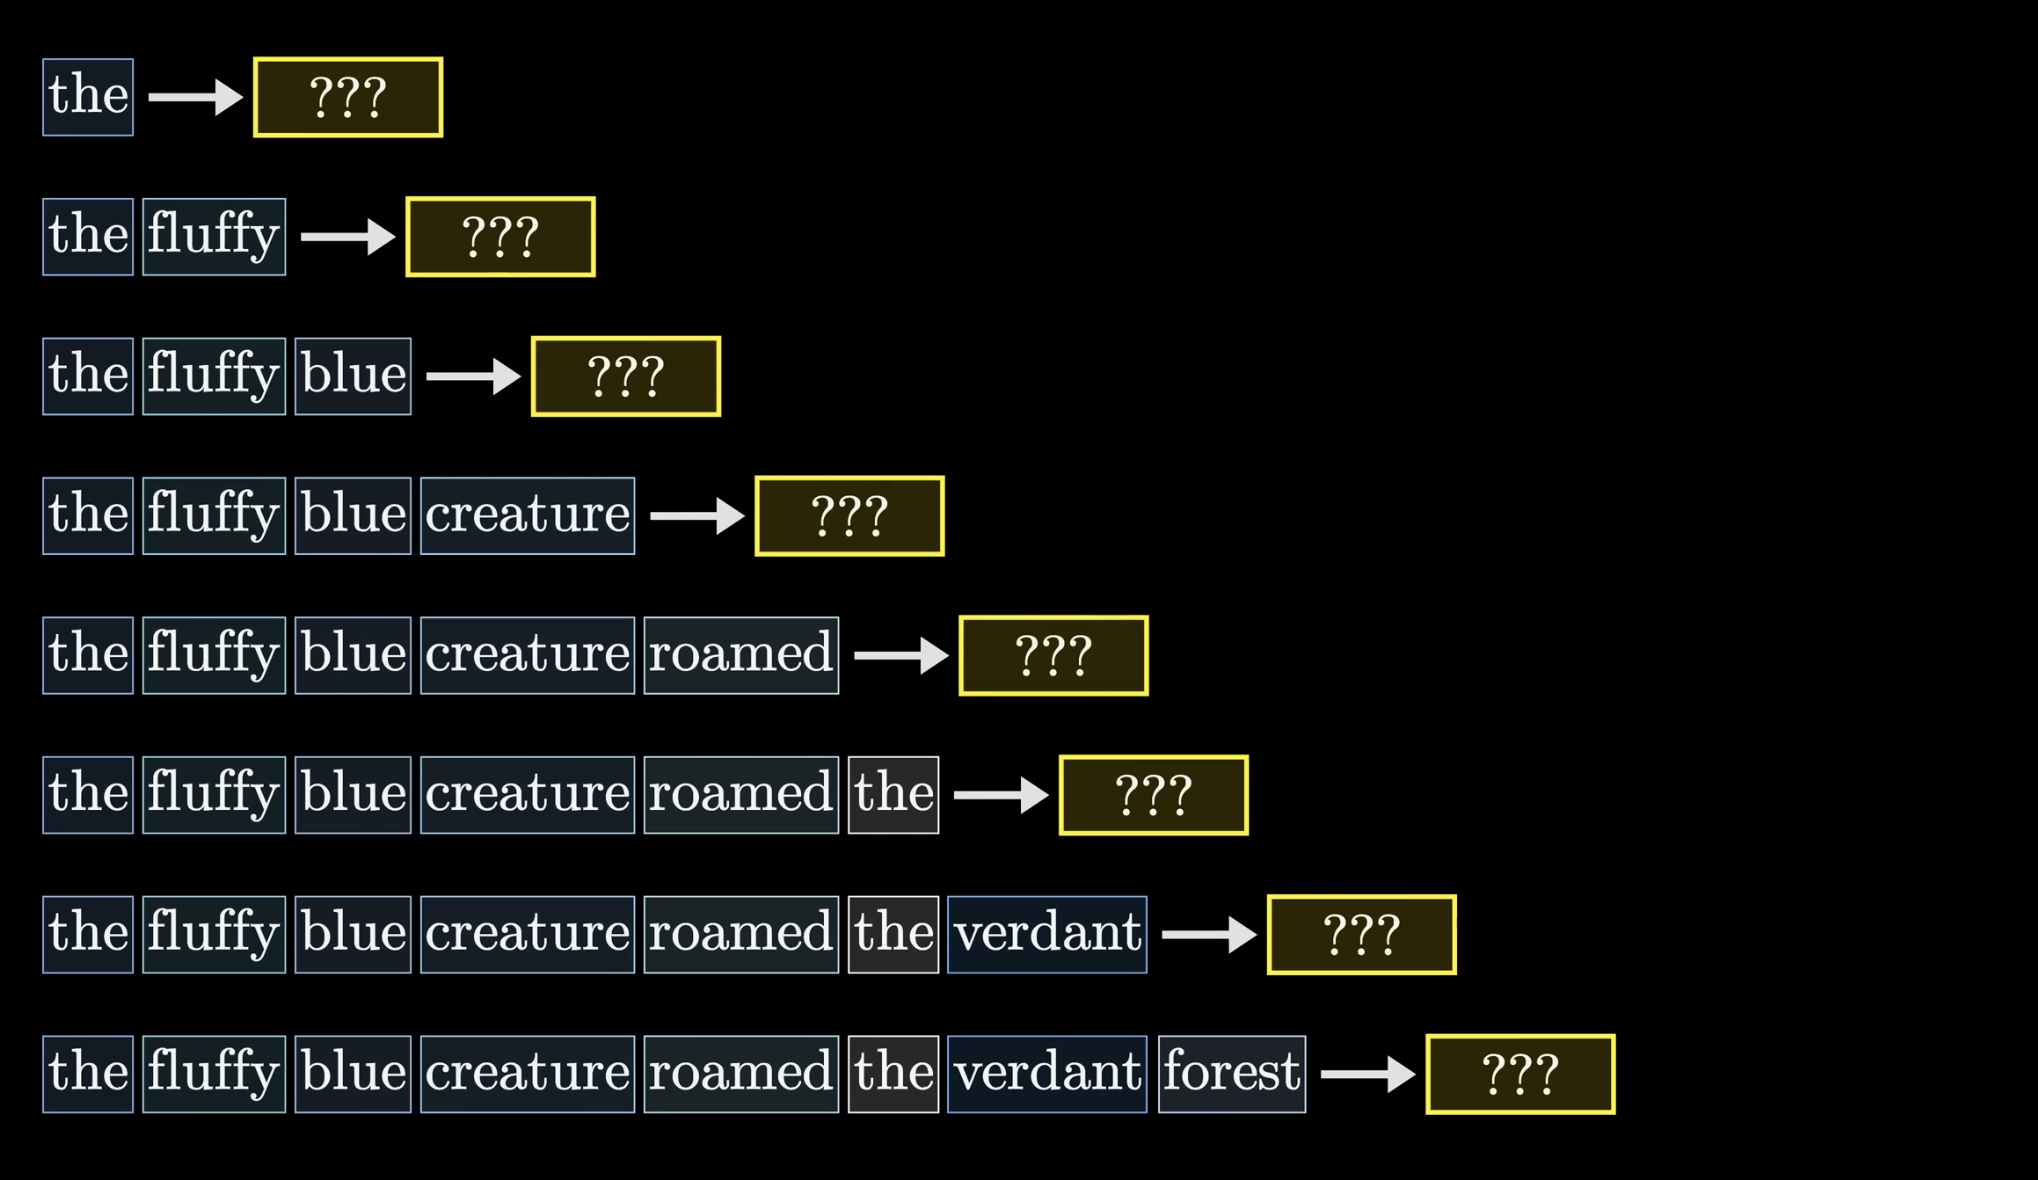
\includegraphics[width=0.85\textwidth]{images/causal_masking1}}
\only<3>{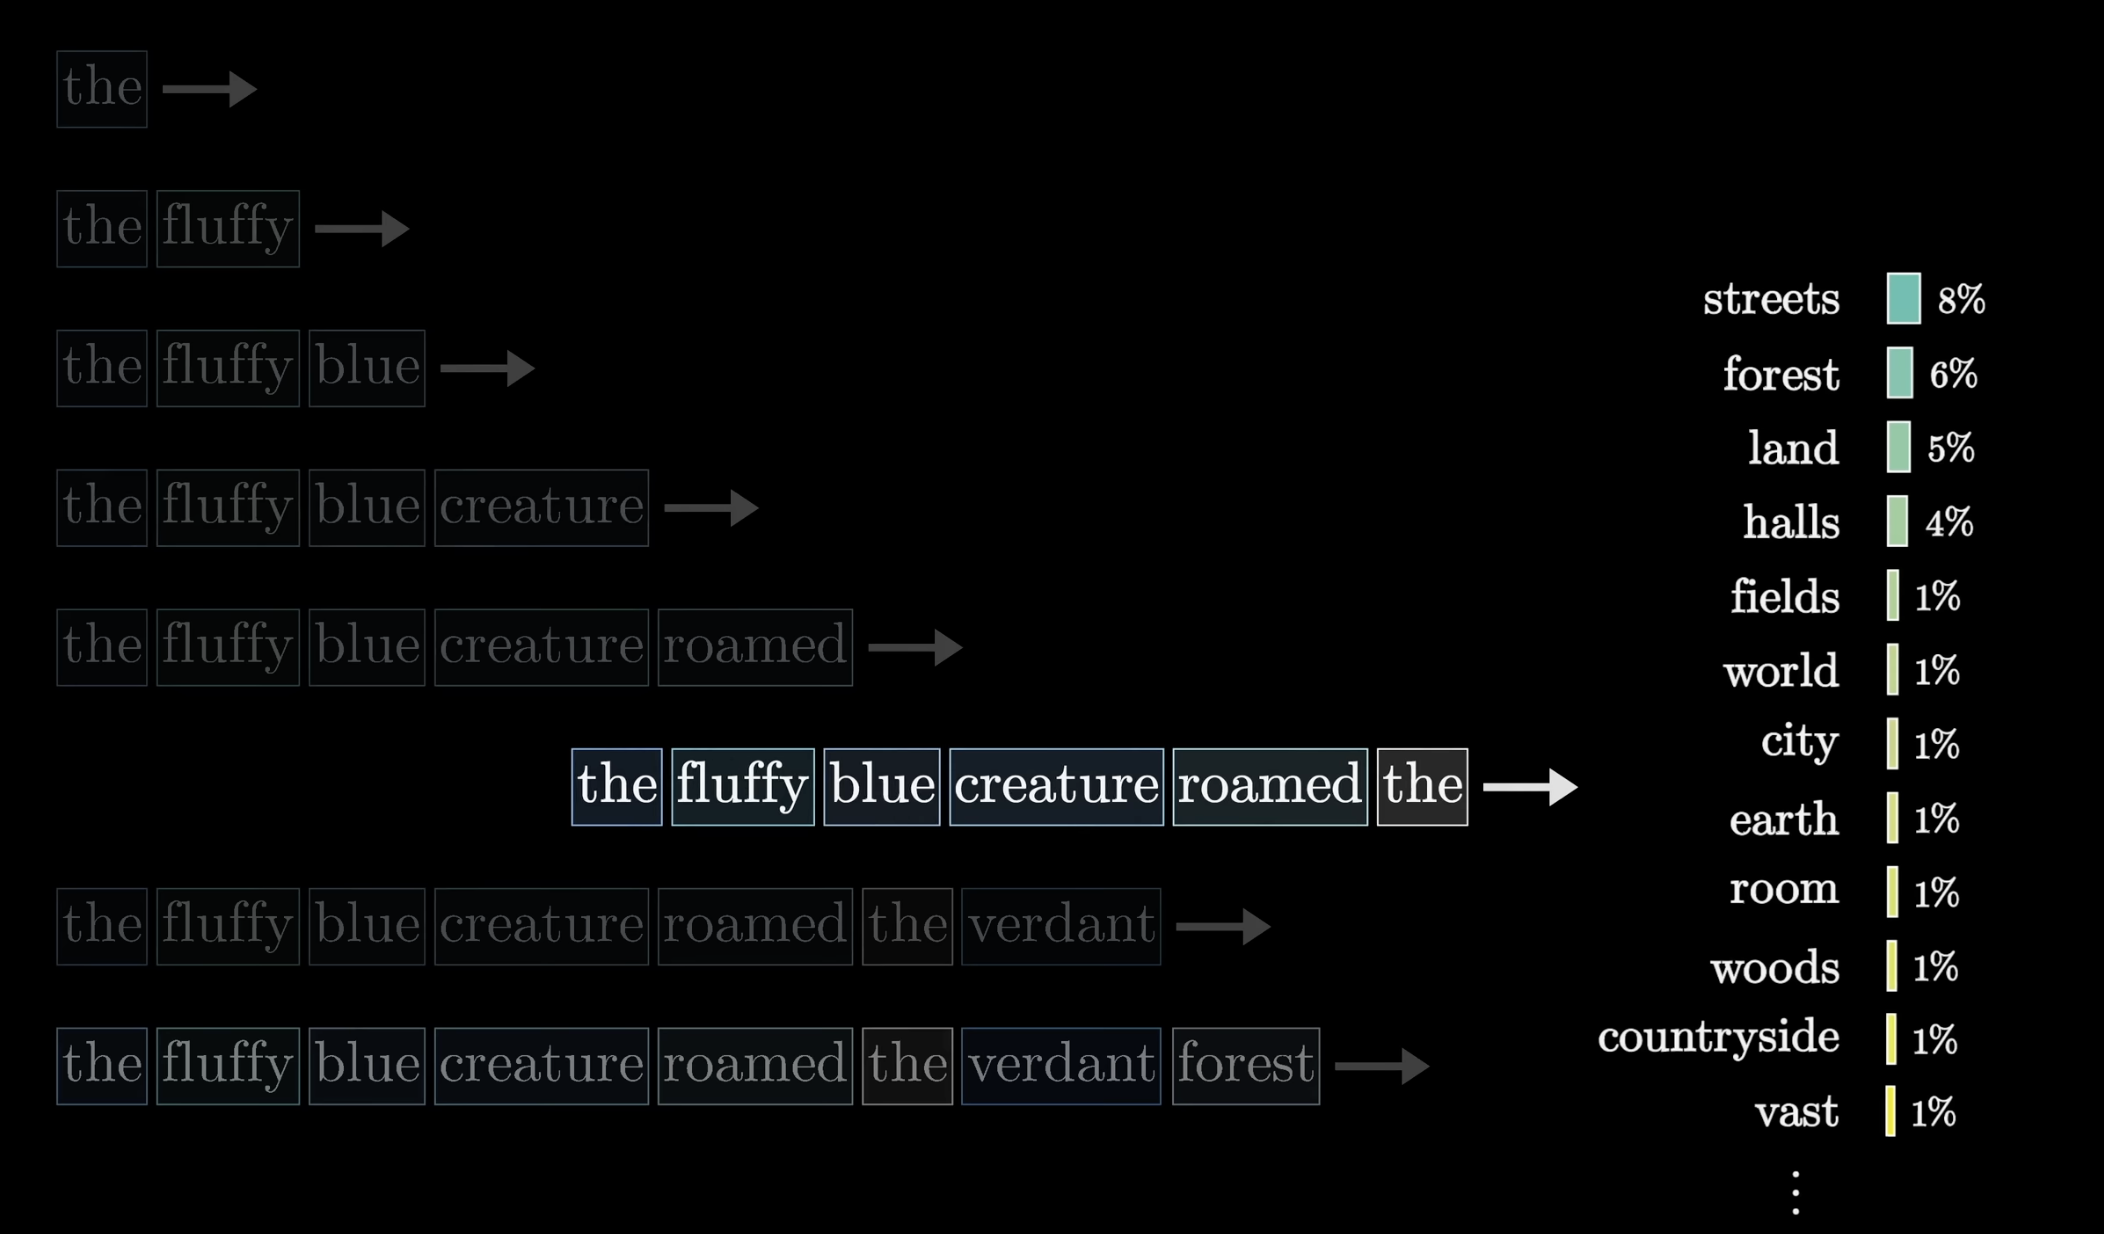
\includegraphics[width=0.85\textwidth]{images/causal_masking2}}
\end{center}
\pause 

The training process is a lot more efficient if you have the model predict every possible next token following each initial subsequence.% of tokens in this passage
\pause 
\begin{itemize}
	\item What would be a single training example effectively acts as many.
\end{itemize}
	
\end{frame}



\begin{frame}{Causal masking}
You never want later words to influence earlier words, since it could \qq{give away} the answer

\pause 
\begin{center}
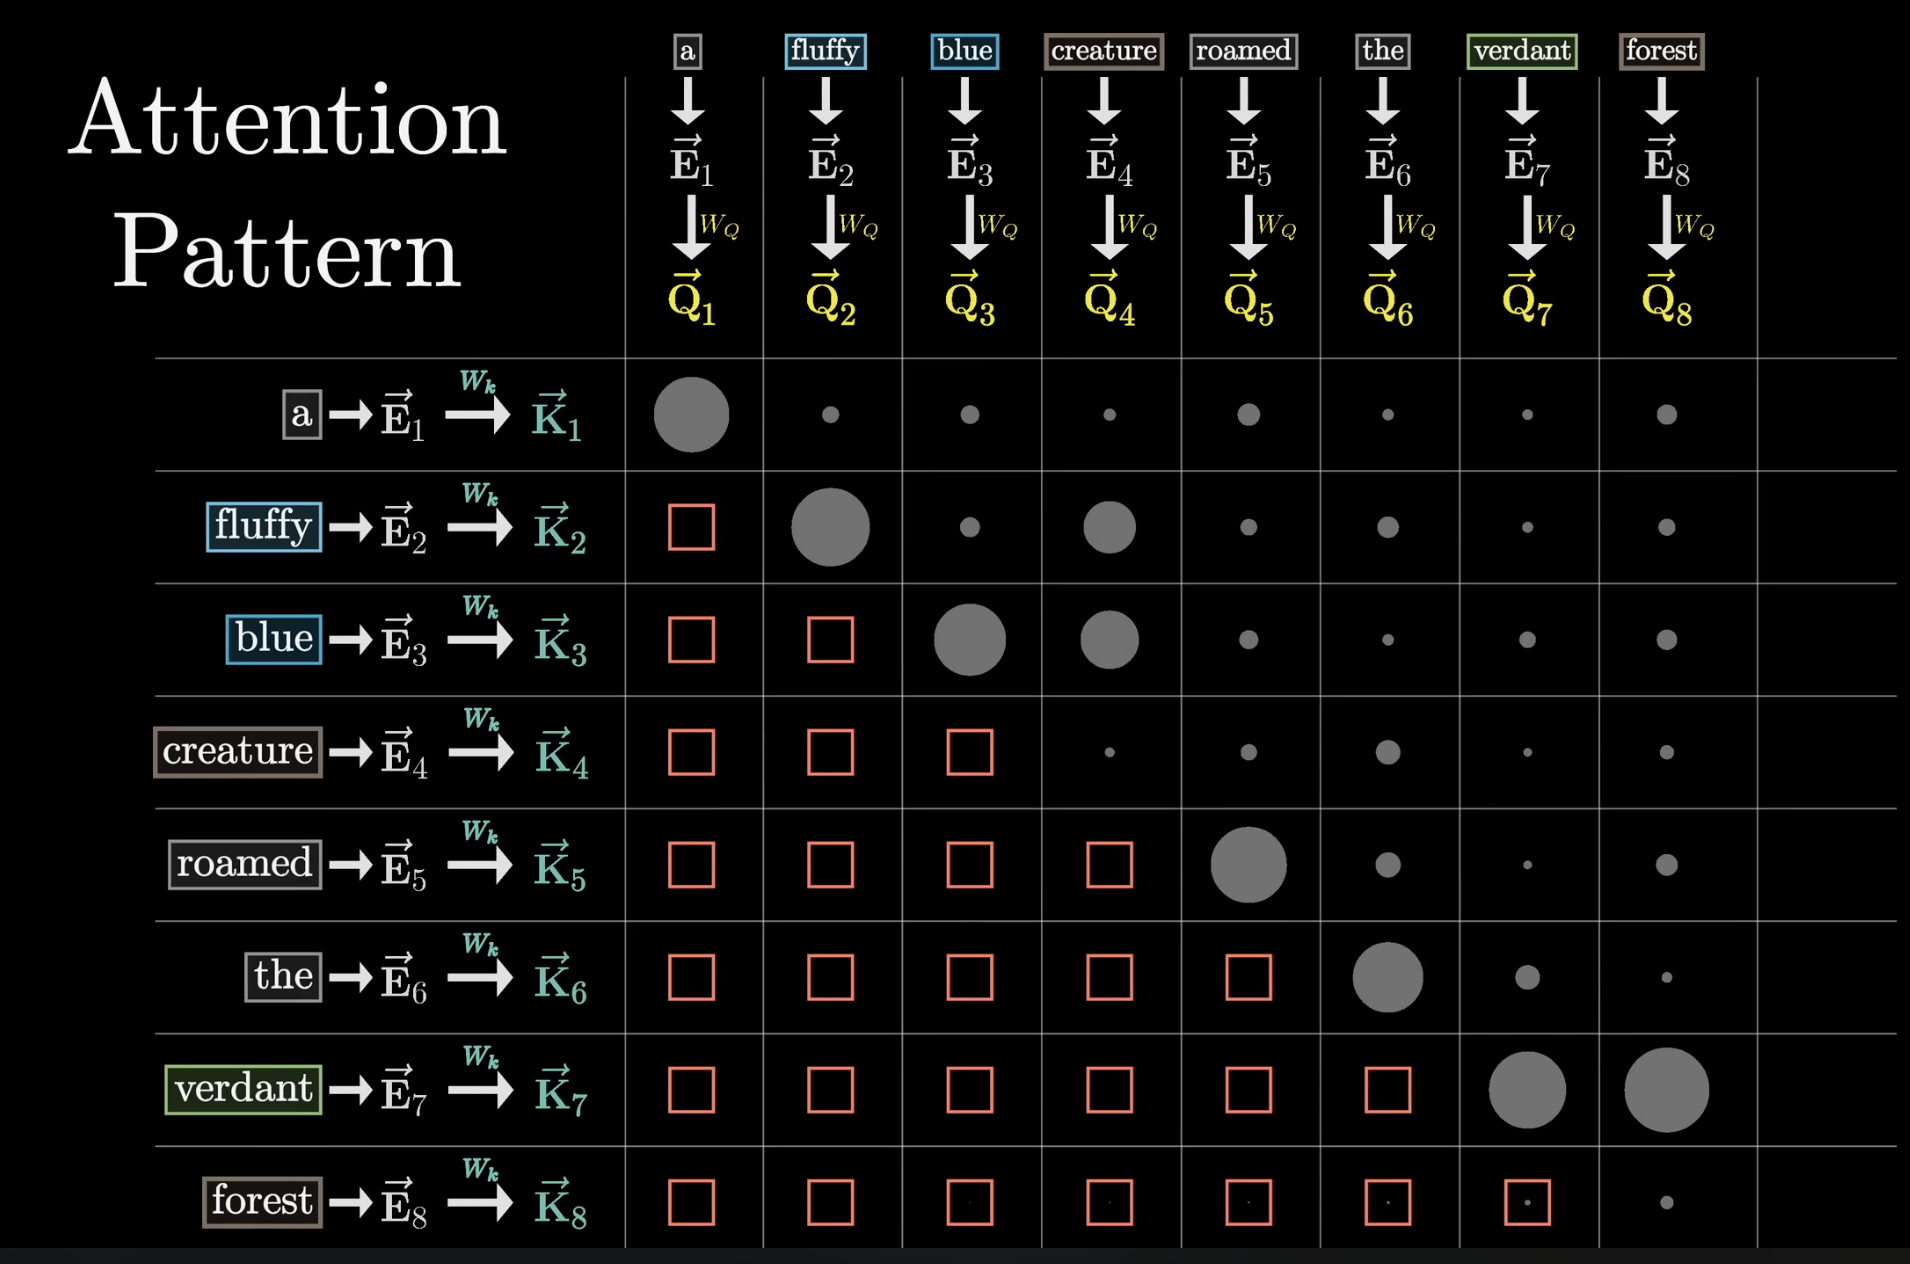
\includegraphics[width=0.85\textwidth]{images/causal_masking3}
\end{center}

\pause 
So you (effectively) force the lower diagonal of the attention pattern to be 0.

\end{frame}

\begin{frame}{Causal masking}
\begin{center}
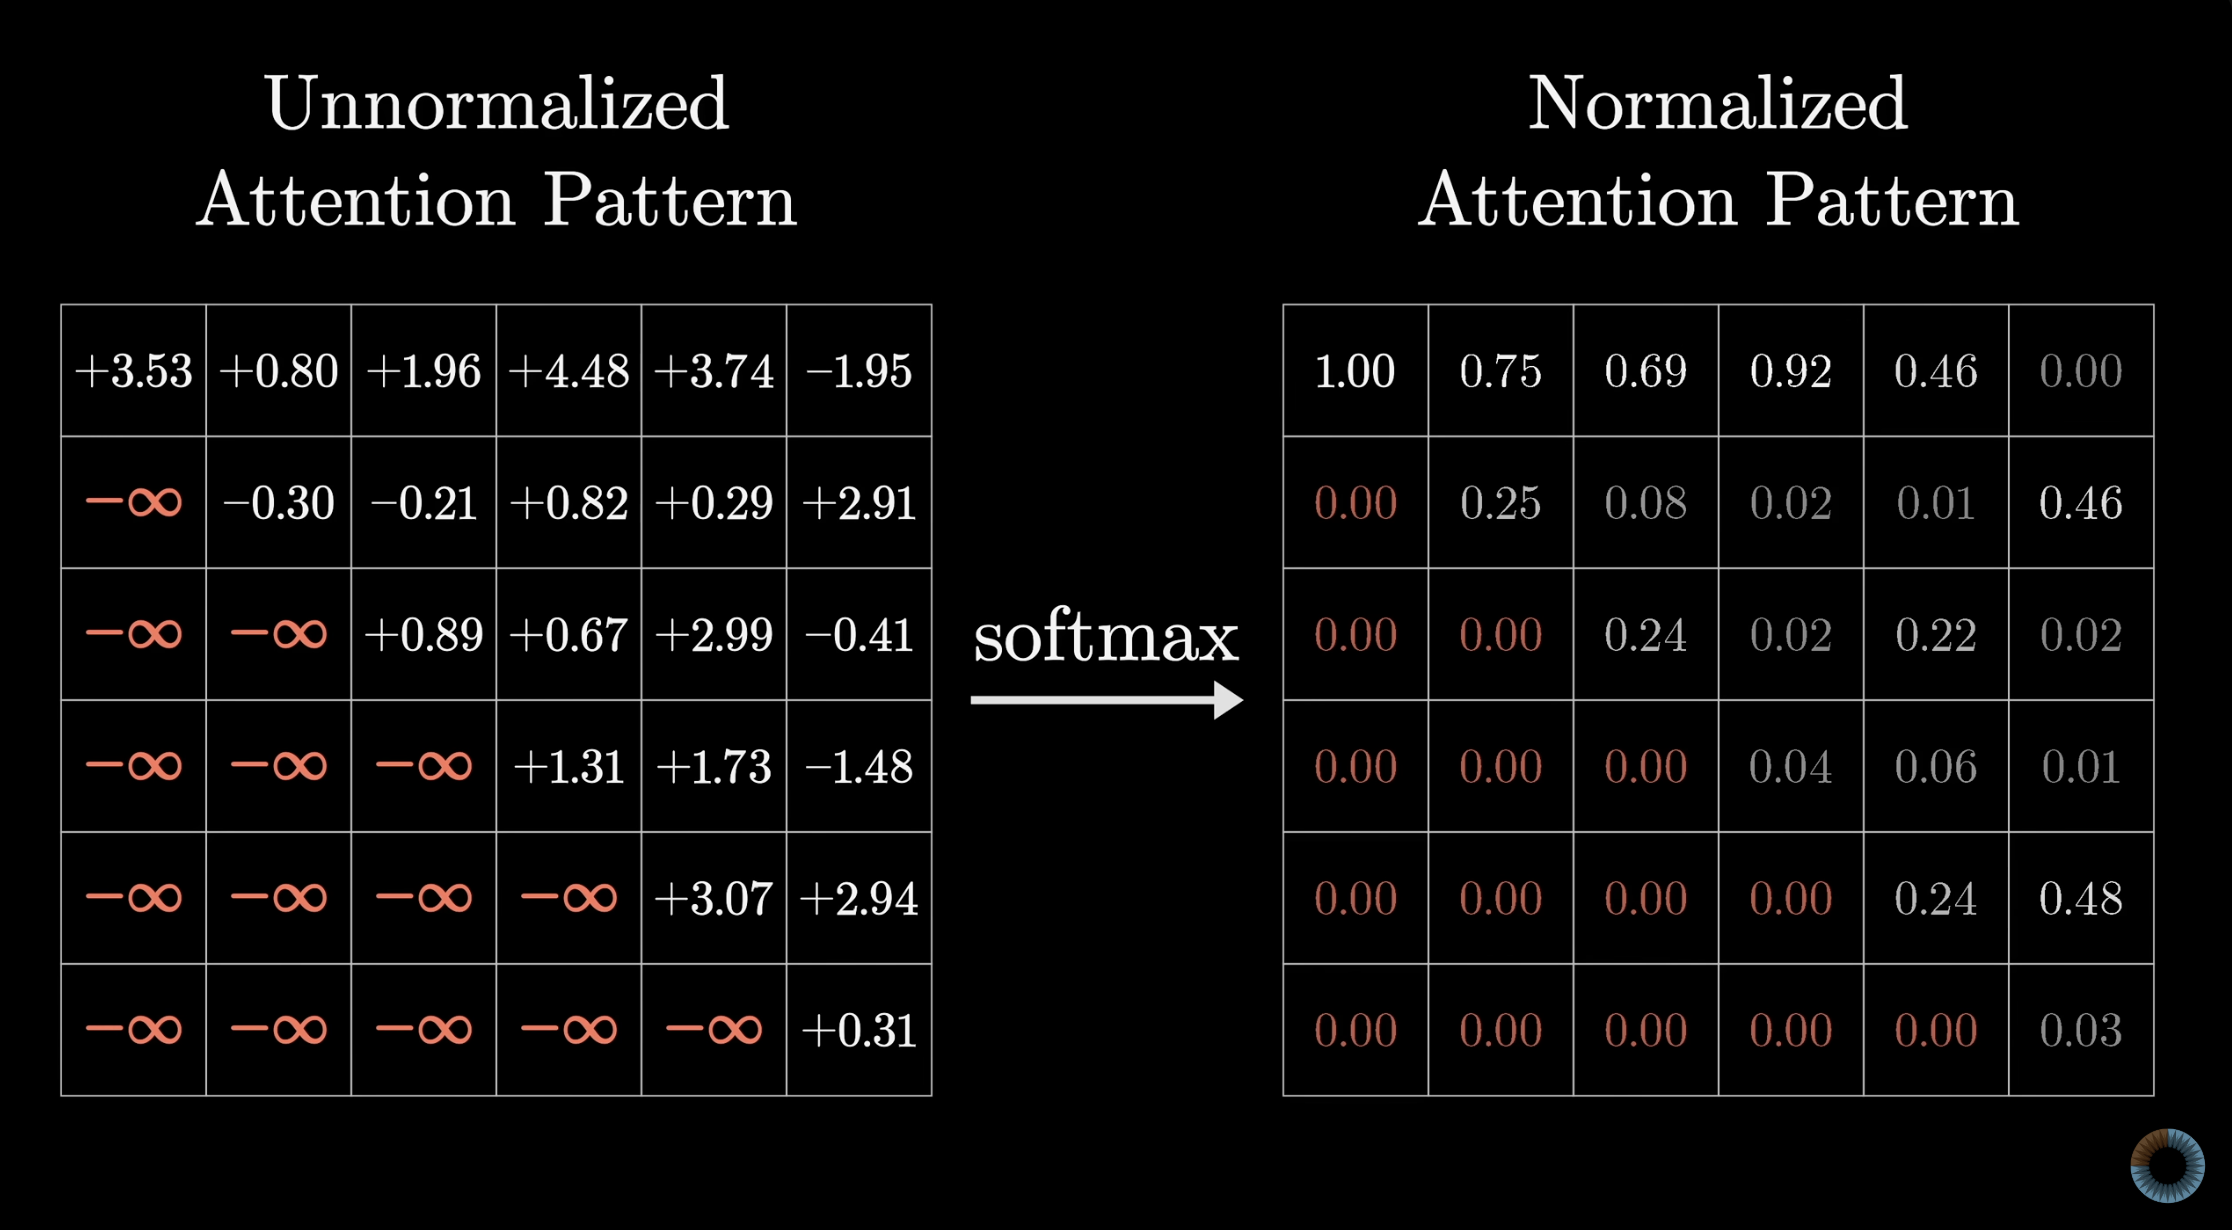
\includegraphics[width=0.85\textwidth]{images/causal_masking4}
\end{center}

\pause 

This is called \alert{causal masking}.

\end{frame}


\begin{frame}{Values}
	
Now that we have the attention pattern, we need to actually \textbf{update the embeddings}.

\begin{center}
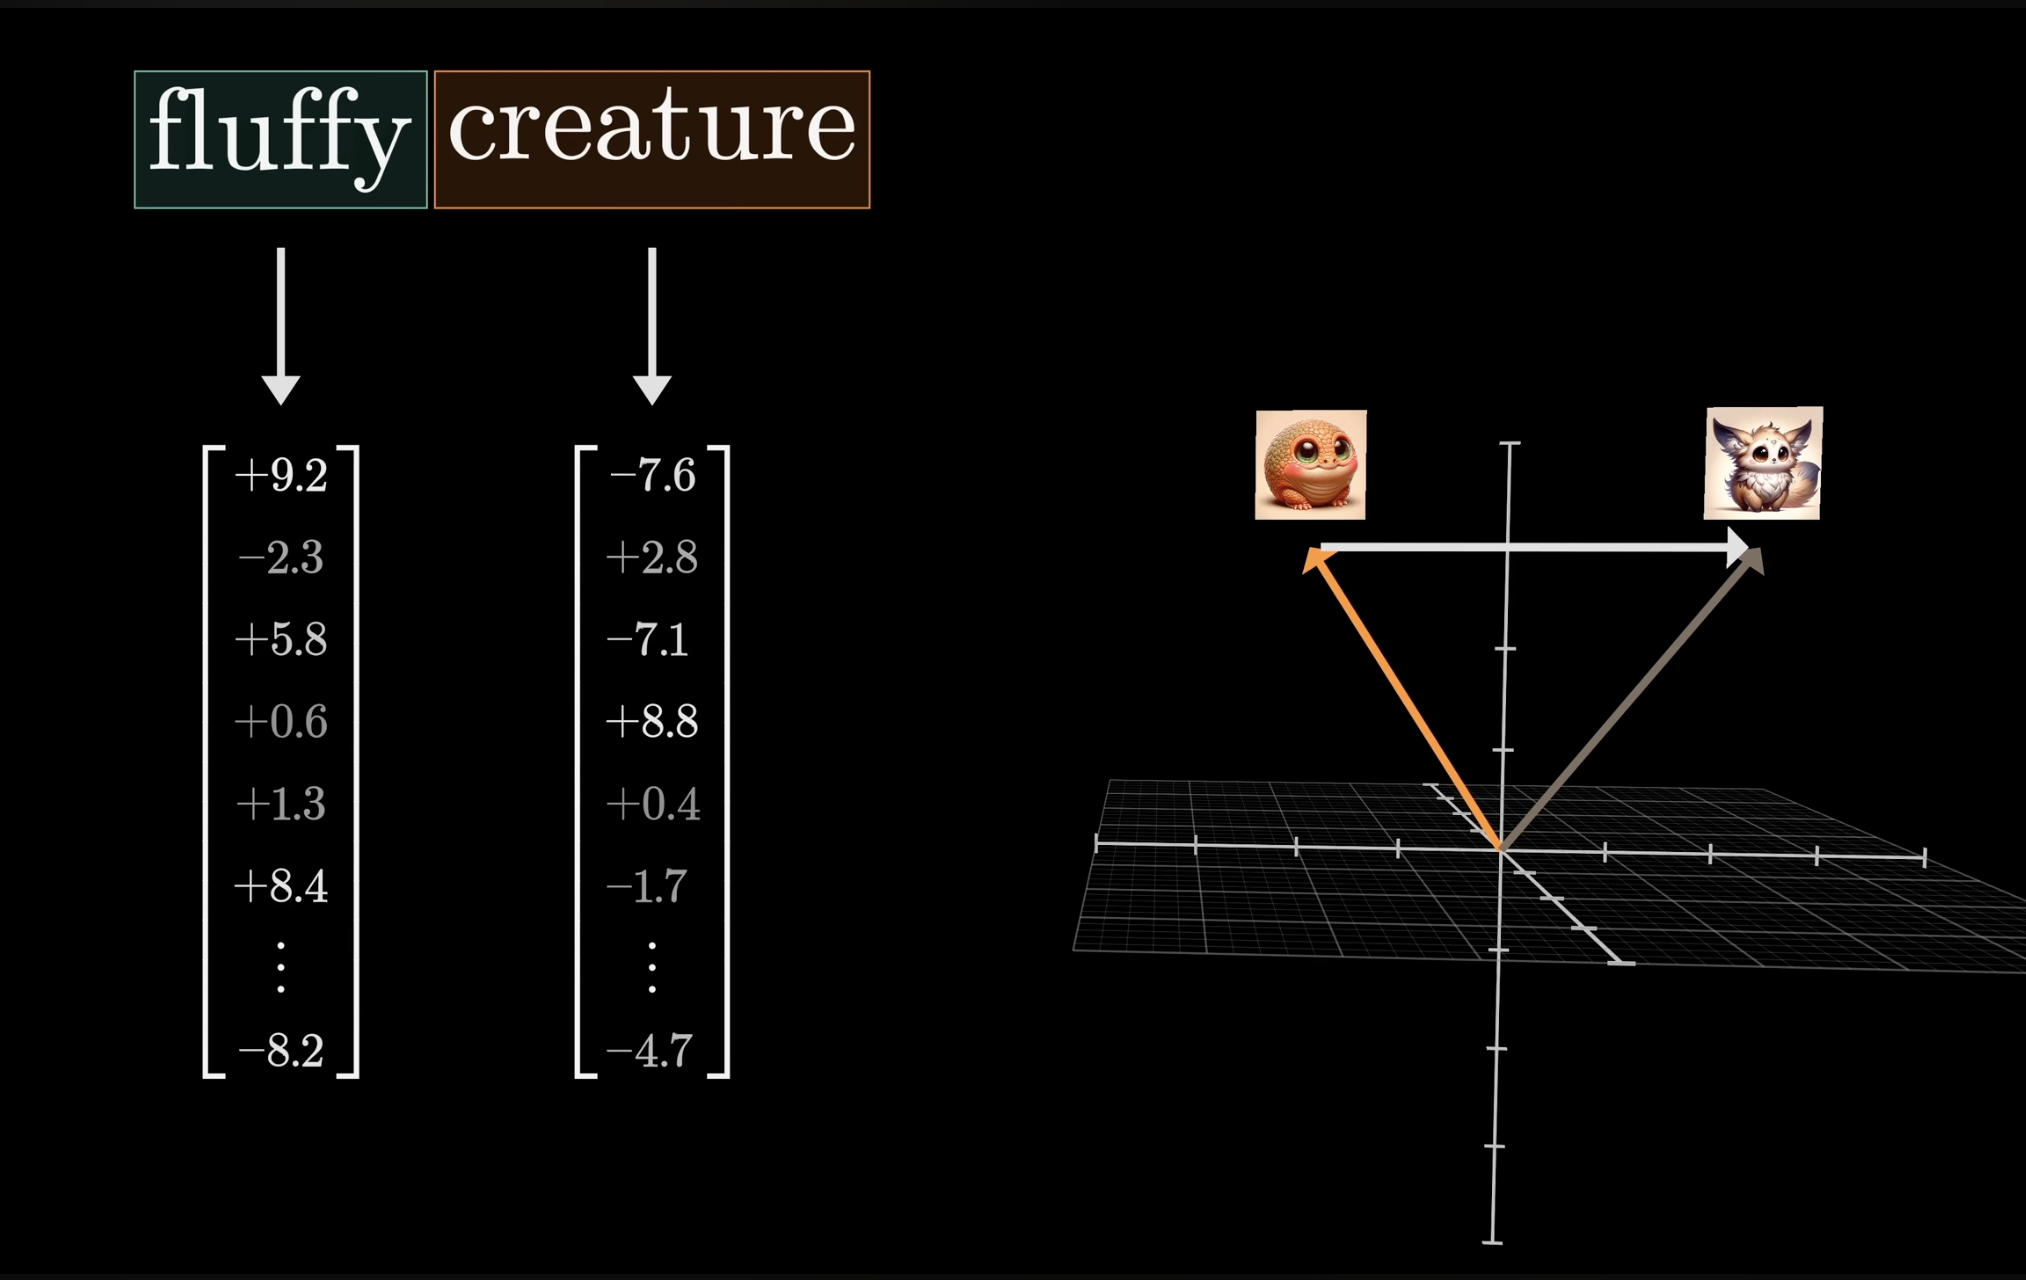
\includegraphics[width=0.85\textwidth]{images/fluffy_creature}
\end{center}

\end{frame}


\begin{frame}{Values}

\small 
\begin{center}


\only<1-3>{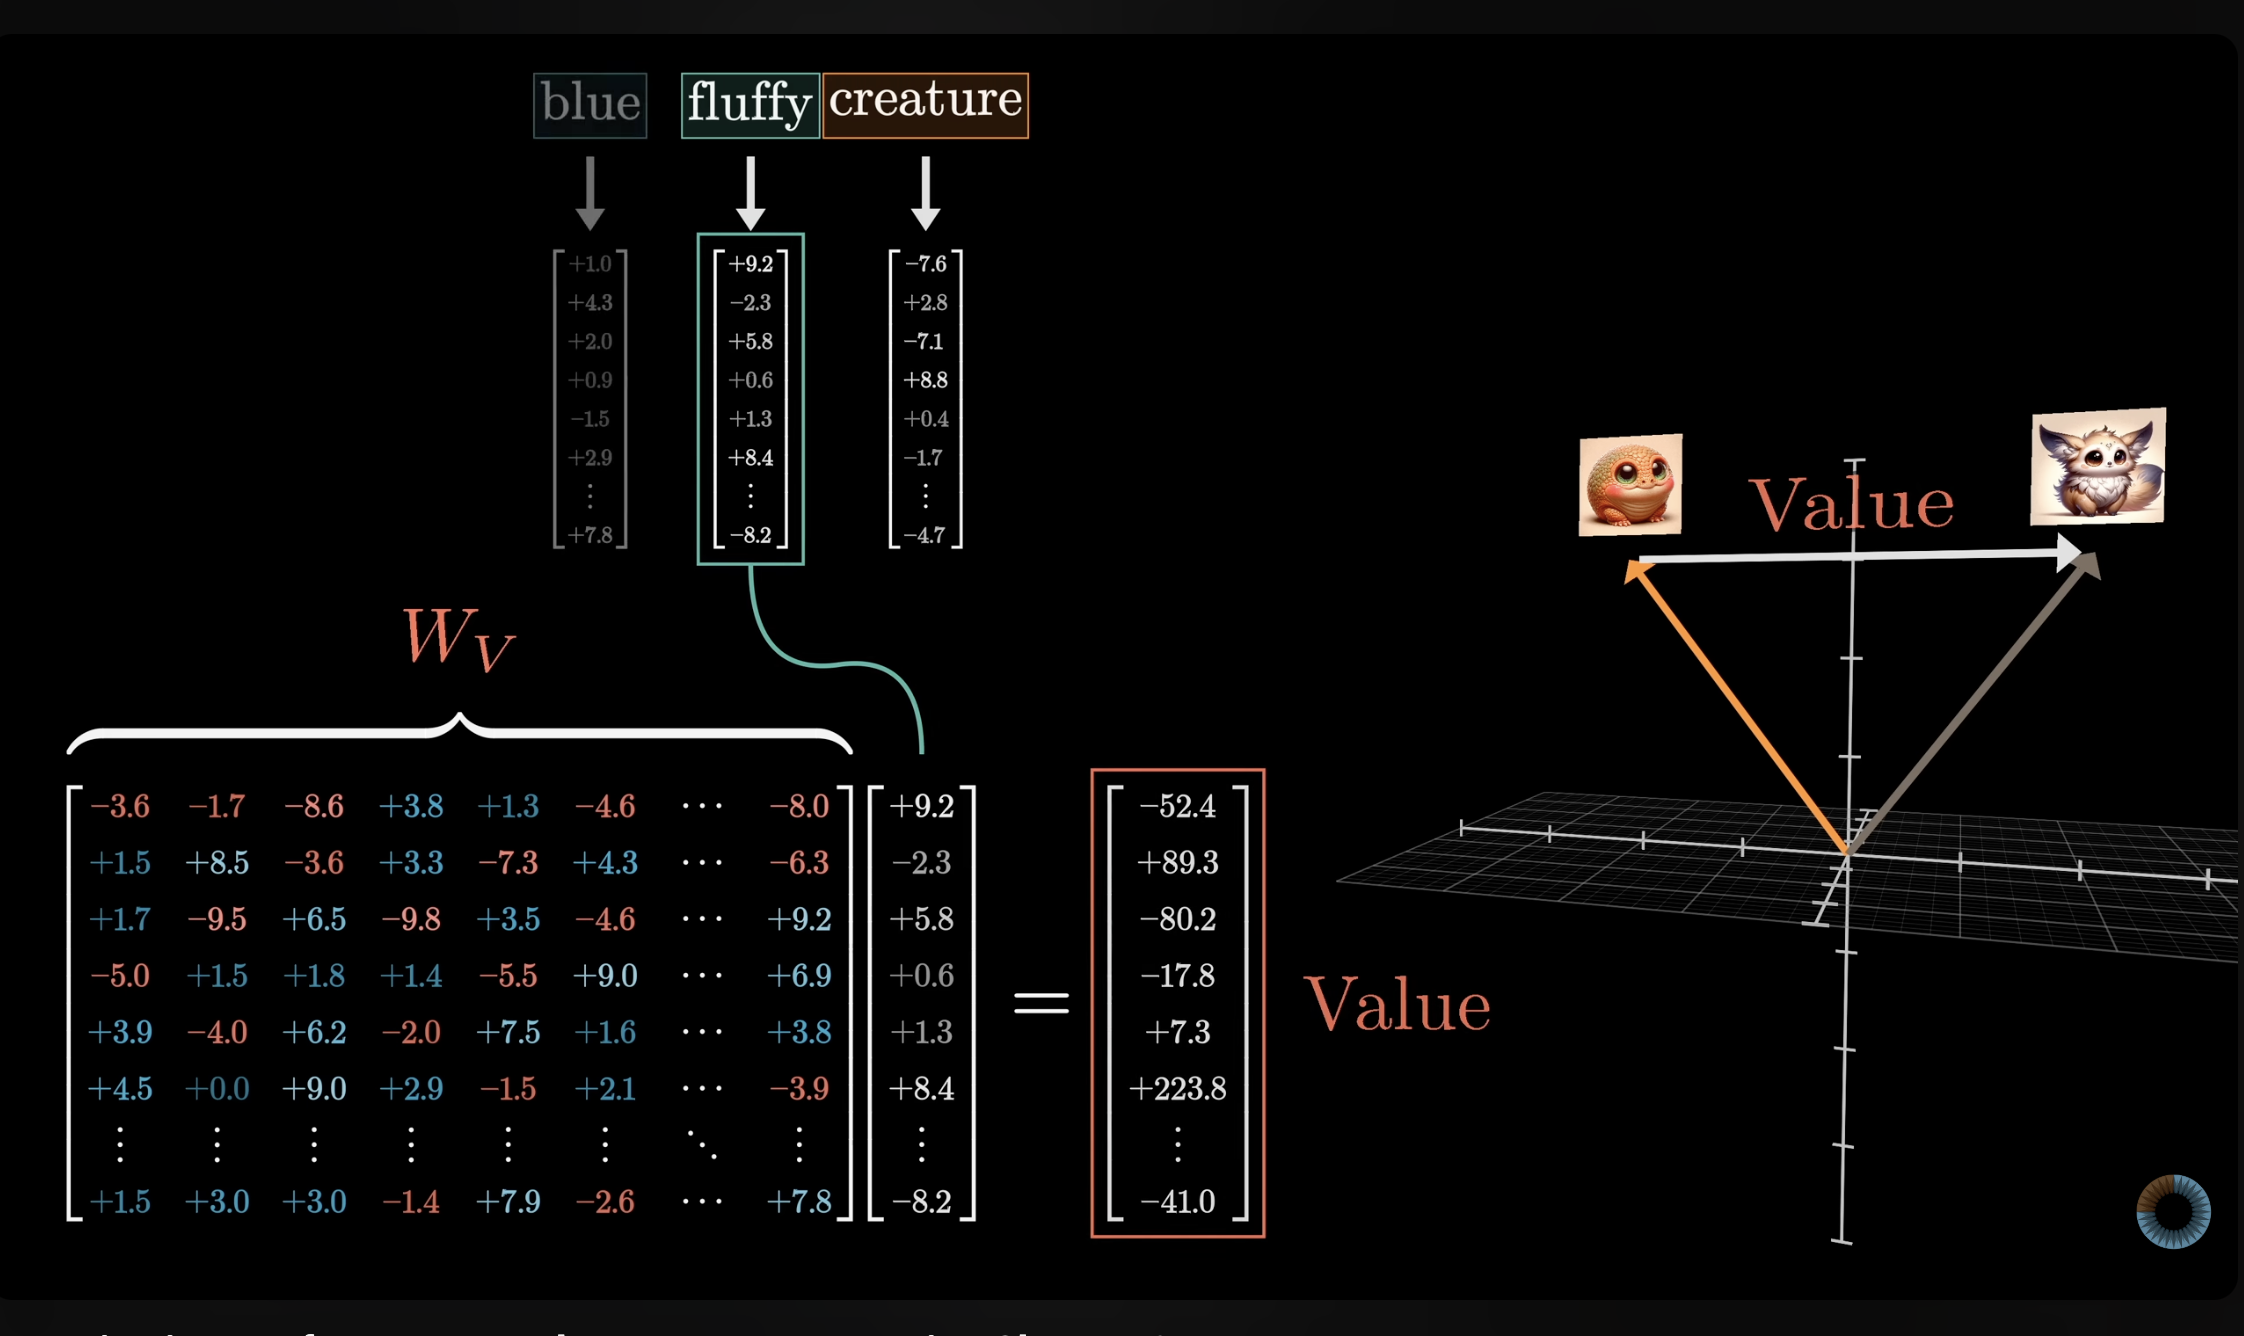
\includegraphics[width=0.8\textwidth]{images/value_1}}


\only<4->{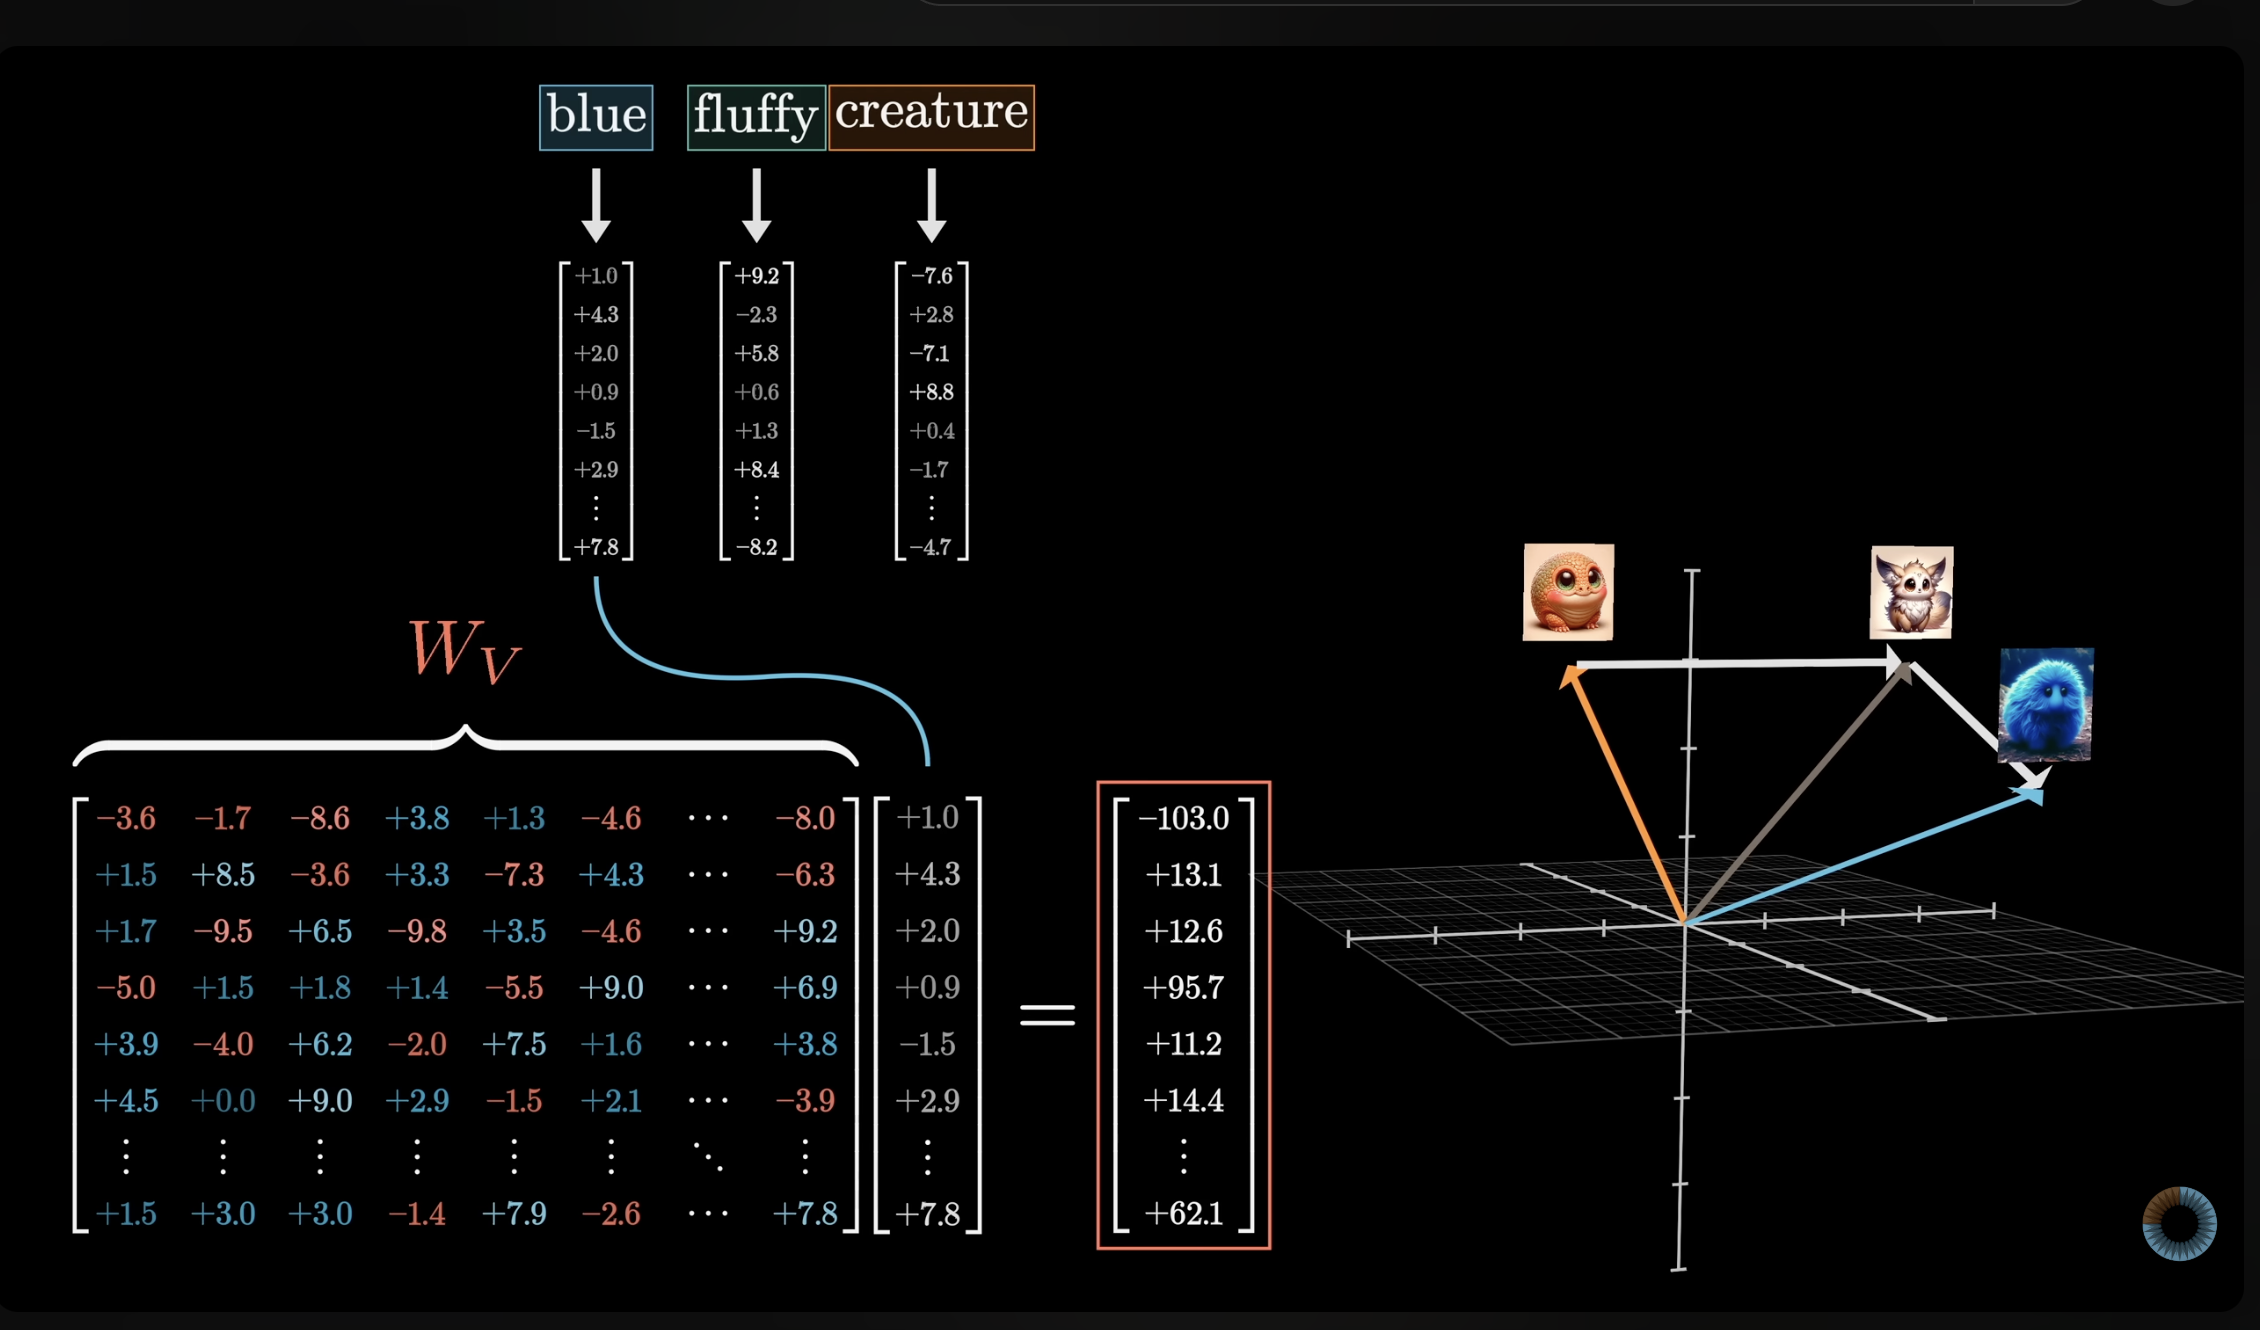
\includegraphics[width=0.8\textwidth]{images/value_2}}

\end{center}


\only<1-4>{
We use a third matrix, called the \alert{value matrix} to  multiply the embeddings (e.g. "fluffy") to create a sequence of values.  }

\only<2-4>{
\begin{itemize}
\item How to get it? $\vec{V}=\+W_V \vec{E}$, where $\+W_V$ is learnable.
\end{itemize}
}

\only<3-4>{
 We then add this value to the embeddings that \qq{fluffy} attends to (e.g. \qq{creature}.)	
}   \only<4-4>{Now we do the same for \qq{blue}.	
} 

\only<5>{ So the \alert{value vector} answers the question: \qq{\underline{If} this word is relevant to adjusting the meaning of something else, what exactly should be added to the embedding of that something else?}

}

\end{frame}




\section{Lightning Chat}

\end{document}

